% -*- latex -*-
%%%%%%%%%%%%%%%%%%%%%%%%%%%%%%%%%%%%%%%%%%%%%%%%%%%%%%%%%%%%%%%%
%%%%%%%%%%%%%%%%%%%%%%%%%%%%%%%%%%%%%%%%%%%%%%%%%%%%%%%%%%%%%%%%
%%%%
%%%% This text file is part of the source of 
%%%% `Introduction to High-Performance Scientific Computing'
%%%% by Victor Eijkhout, copyright 2012-8
%%%%
%%%% This book is distributed under a Creative Commons Attribution 3.0
%%%% Unported (CC BY 3.0) license and made possible by funding from
%%%% The Saylor Foundation \url{http://www.saylor.org}.
%%%%
%%%%
%%%%%%%%%%%%%%%%%%%%%%%%%%%%%%%%%%%%%%%%%%%%%%%%%%%%%%%%%%%%%%%%
%%%%%%%%%%%%%%%%%%%%%%%%%%%%%%%%%%%%%%%%%%%%%%%%%%%%%%%%%%%%%%%%

The largest and most powerful computers are sometimes called
`supercomputers'. For the last two decades, this has, without
exception, referred to parallel computers: machines with more than one
CPU that can be set to work on the same problem.

Parallelism is hard to define precisely, since it can appear on
several levels. In the previous chapter you already saw how inside a
CPU several instructions can be `in flight' simultaneously. This is
called \indextermsub{instruction-level}{parallelism}, and it is outside
explicit user control: it derives from the compiler and the CPU
deciding which instructions, out of a single instruction stream, can
be processed simultaneously. At the other extreme is the sort of
parallelism where more than one instruction stream is handled by
multiple processors, often each on their own circuit board. This type
of parallelism is typically explicitly scheduled by the user.

In this chapter, we will analyze this more explicit type of
parallelism, the hardware that supports it, the programming that
enables it, and the concepts that analyze it.

\Level 0 {Introduction}
\label{sec:parallel-intro}

In scientific codes, there is often a large amount of work to be done,
and it is often regular to some extent, with the same operation being
performed on many data. The question is then whether this work can be
sped up by use of a parallel computer. If there are $n$ operations to
be done, and they would take time~$t$ on a single processor, can they
be done in time~$t/p$ on $p$~processors?

Let us start with a very simple example. Adding two vectors of length~$n$
\begin{verbatim}
for (i=0; i<n; i++)
  a[i] = b[i] + c[i];
\end{verbatim}
can be done with up to $n$~processors. In the idealized case with $n$
processors, each processor has local scalars \n{a,b,c} and executes
\begin{figure}[ht]
  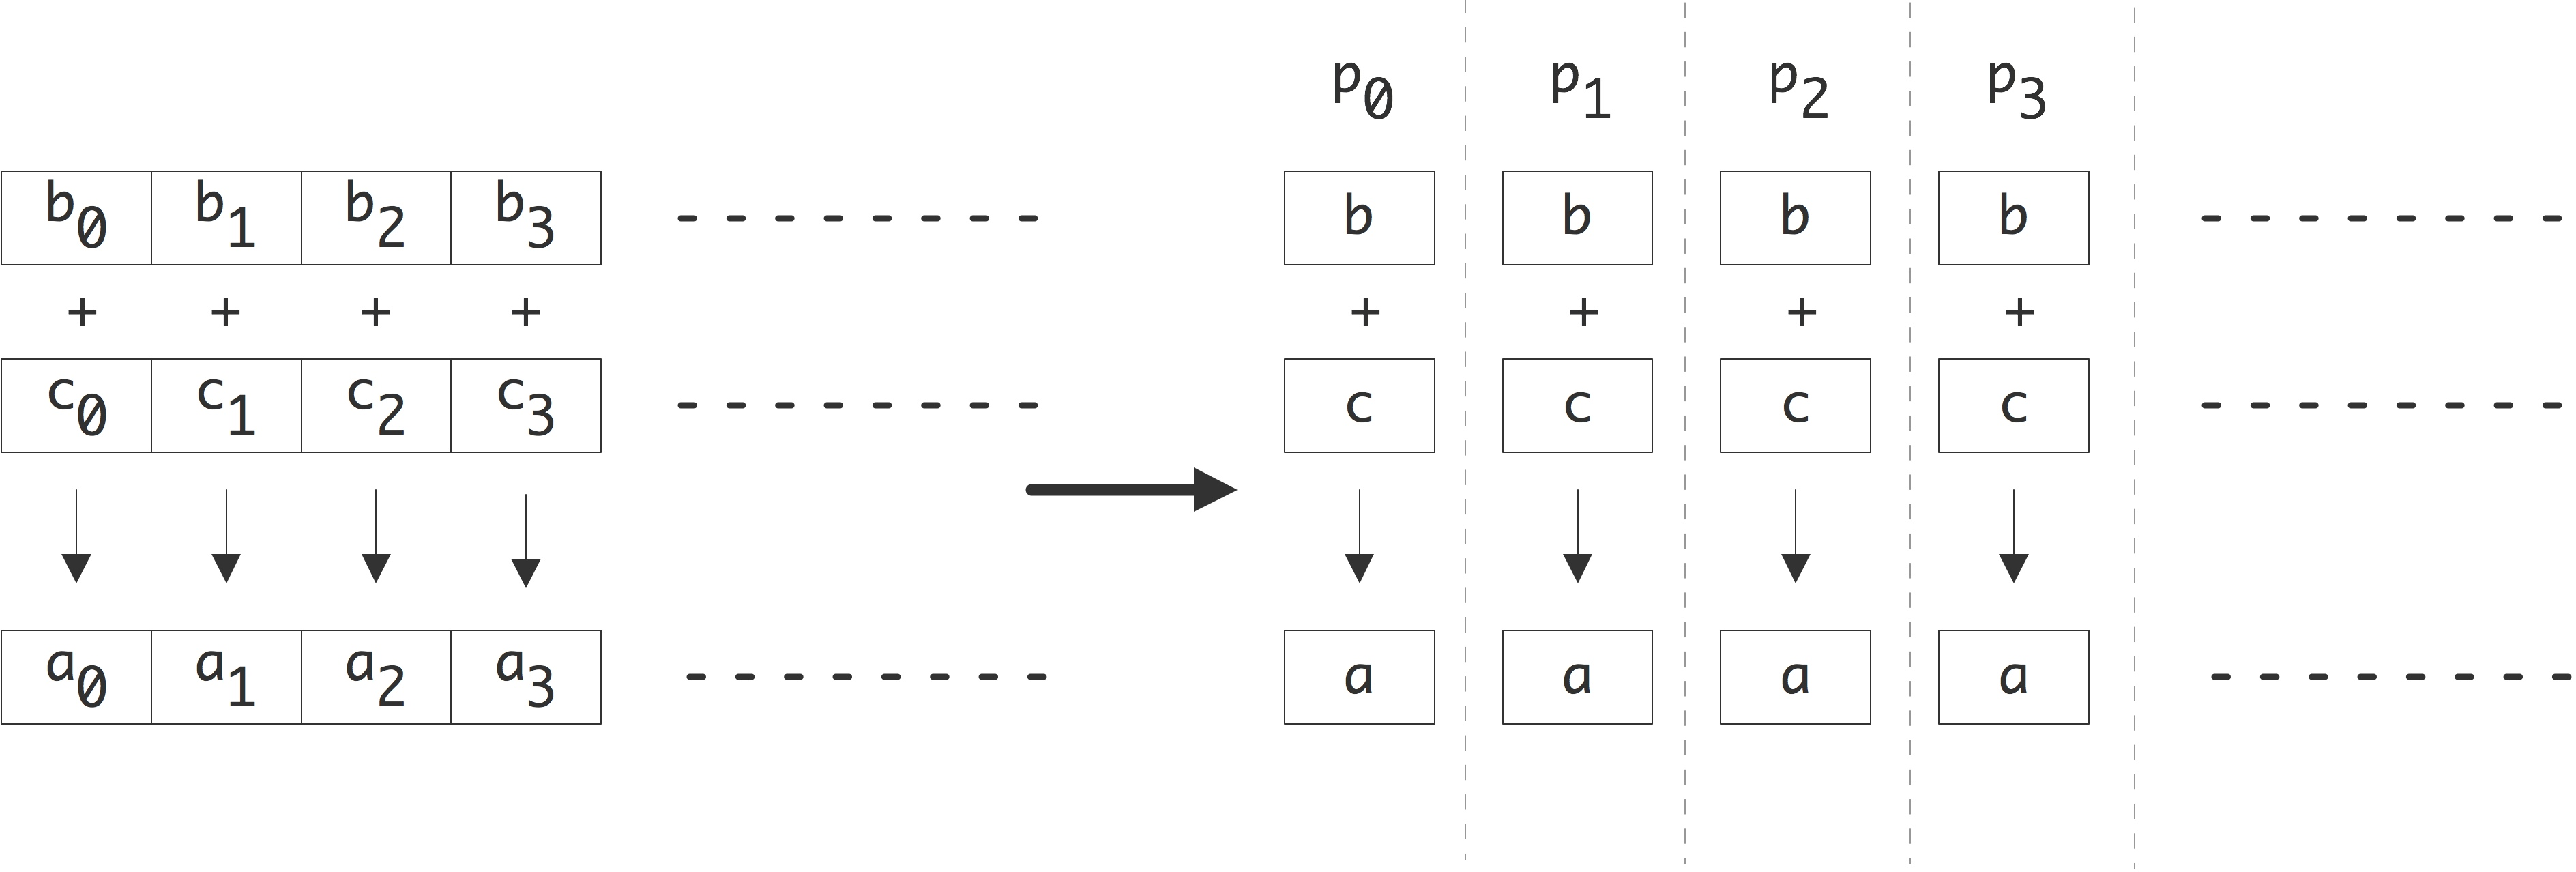
\includegraphics[scale=.11]{graphics/parallel-add}
  \caption{Parallelization of a vector addition}
  \label{fig:par-add}
\end{figure}
the single instruction \n{a=b+c}. This is depicted in
figure~\ref{fig:par-add}.

In the general case, where each processor executes something like
\begin{verbatim}
for (i=my_low; i<my_high; i++)
  a[i] = b[i] + c[i];
\end{verbatim}
execution time is linearly
reduced with the number of processors. If each operation takes a unit
time, the original algorithm takes time~$n$, and the parallel
execution on $p$ processors~$n/p$. The parallel algorithm is faster by
a factor of~$p$\footnote{We ignore lower order errors in this result
  when $p$ does not divide perfectly in~$n$. We will also, in general,
ignore matters of loop overhead.}.

Next, let us consider summing the elements of a vector.
(An operation that has a vector as input but only a scalar as output
is often called a \indexterm{reduction}.)
We again
assume that each processor contains just a single array element. The
sequential code:
\begin{verbatim}
s = 0;
for (i=0; i<n; i++)
  s += x[i]
\end{verbatim}
is no longer obviously parallel, but if we recode the loop as
\begin{verbatim}
for (s=2; s<2*n; s*=2)
  for (i=0; i<n-s/2; i+=s)
    x[i] += x[i+s/2]
\end{verbatim}
there is a way to parallelize it: every iteration of the outer loop is
now a loop that can be done by $n/s$ processors in parallel. Since the
\begin{figure}[ht]
  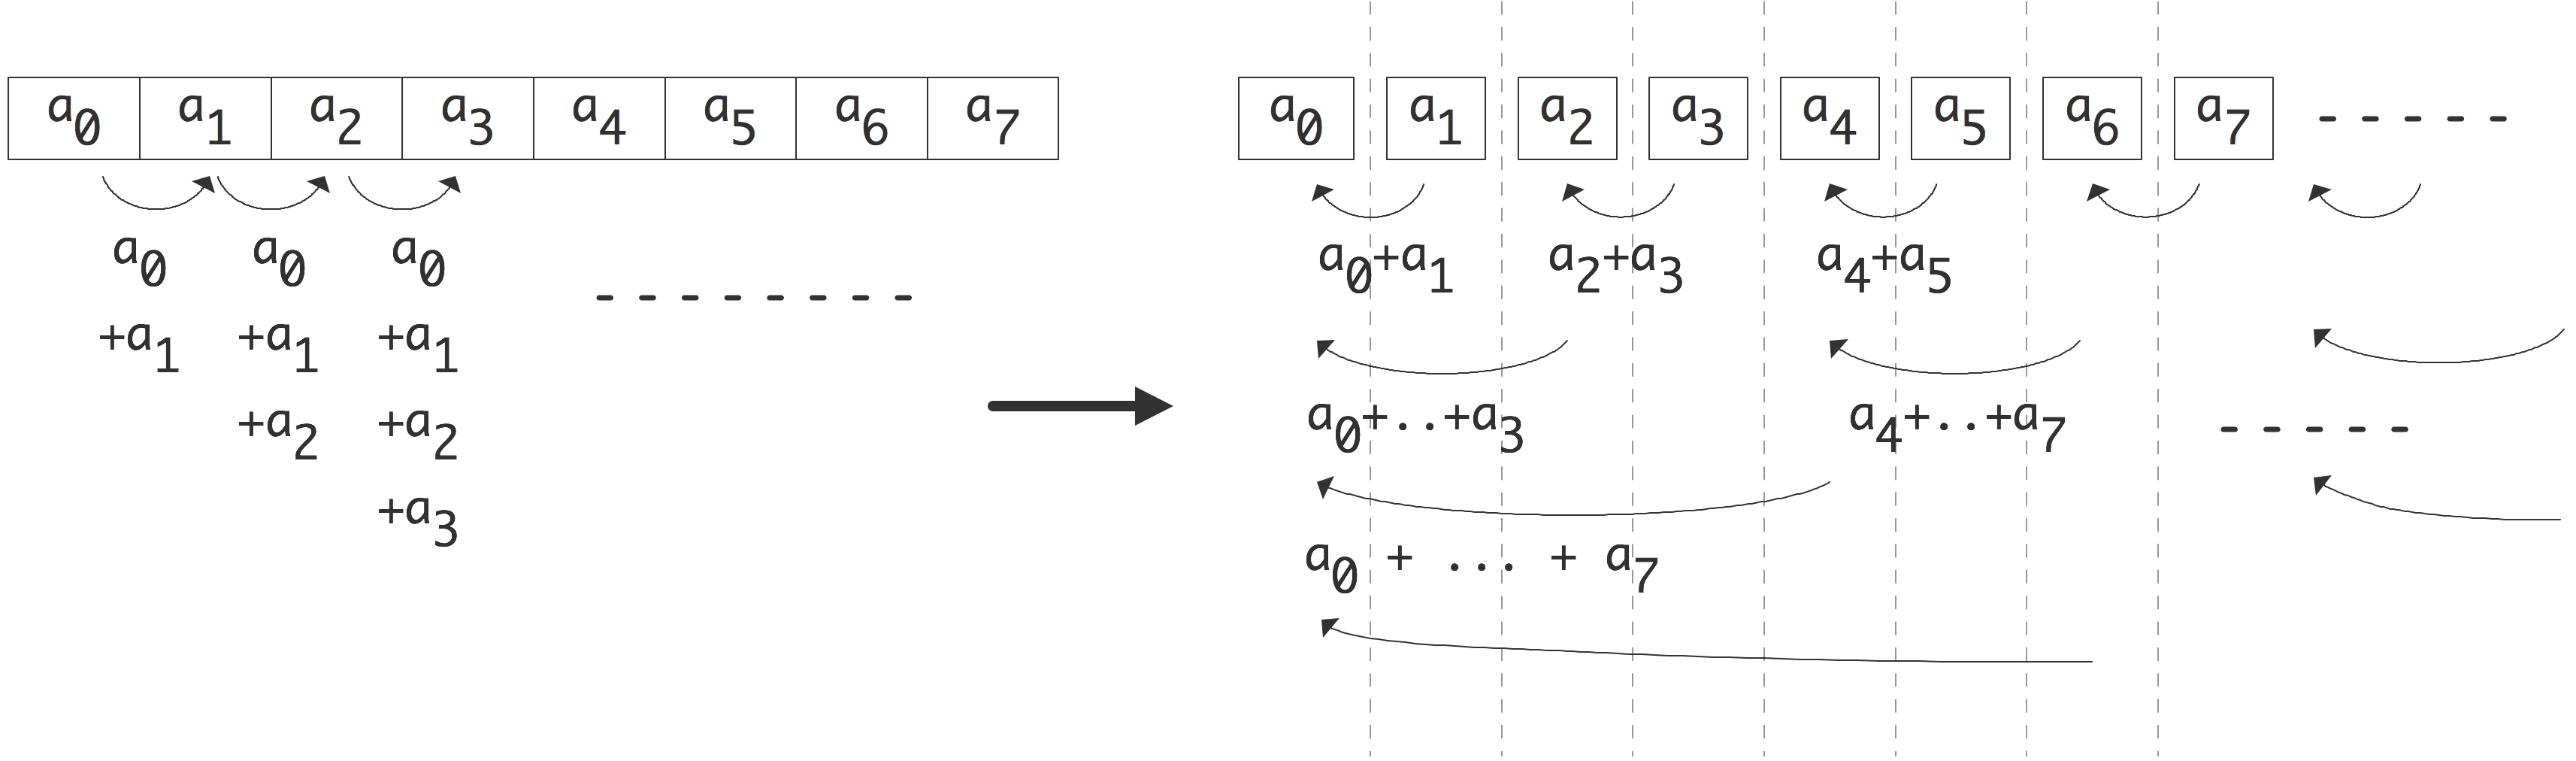
\includegraphics[scale=.13]{graphics/parallel-sum}
  \caption{Parallelization of a vector reduction}
  \label{fig:par-sum}
\end{figure}
outer loop will go through $\log_2n$ iterations, we see that the new
algorithm has a reduced runtime of $n/p\cdot\log_2 n$. The parallel
algorithm is now faster by a factor of $p/\log_2n$. This is depicted
in figure~\ref{fig:par-sum}.

Even from these two simple examples we can see some of the
characteristics of parallel computing:
\begin{itemize}
\item Sometimes algorithms need to be rewritten slightly to make them
  parallel.
\item A parallel algorithm may not show perfect speedup.
\end{itemize}
There are other things to remark on. In the first case, if each
processors has its $x_i,y_i$ in a local store the
algorithm can be executed without further complications. In the second
case, processors need to \emph{communicate} data among each
other and we haven't assigned a cost to that yet.

First let us look systematically at communication. We can take the
parallel algorithm in the right half
of figure~\ref{fig:par-sum} and turn it into a tree graph
(see Appendix~\ref{app:graph}) by defining the inputs as leave nodes,
all partial sums as interior nodes, and the root as the total
sum. There is an edge from one node to another if the first is input
to the (partial) sum in the other. This is illustrated in
figure~\ref{fig:par-sum-graph}. In this figure nodes are horizontally
aligned with other computations that can be performed simultaneously;
each level is sometimes called a \indexterm{superstep} in the computation.
Nodes are vertically aligned if they are computed on the same
processors, and an arrow corresponds to a communication if it goes
from one processor to another. 
\begin{figure}[ht]
  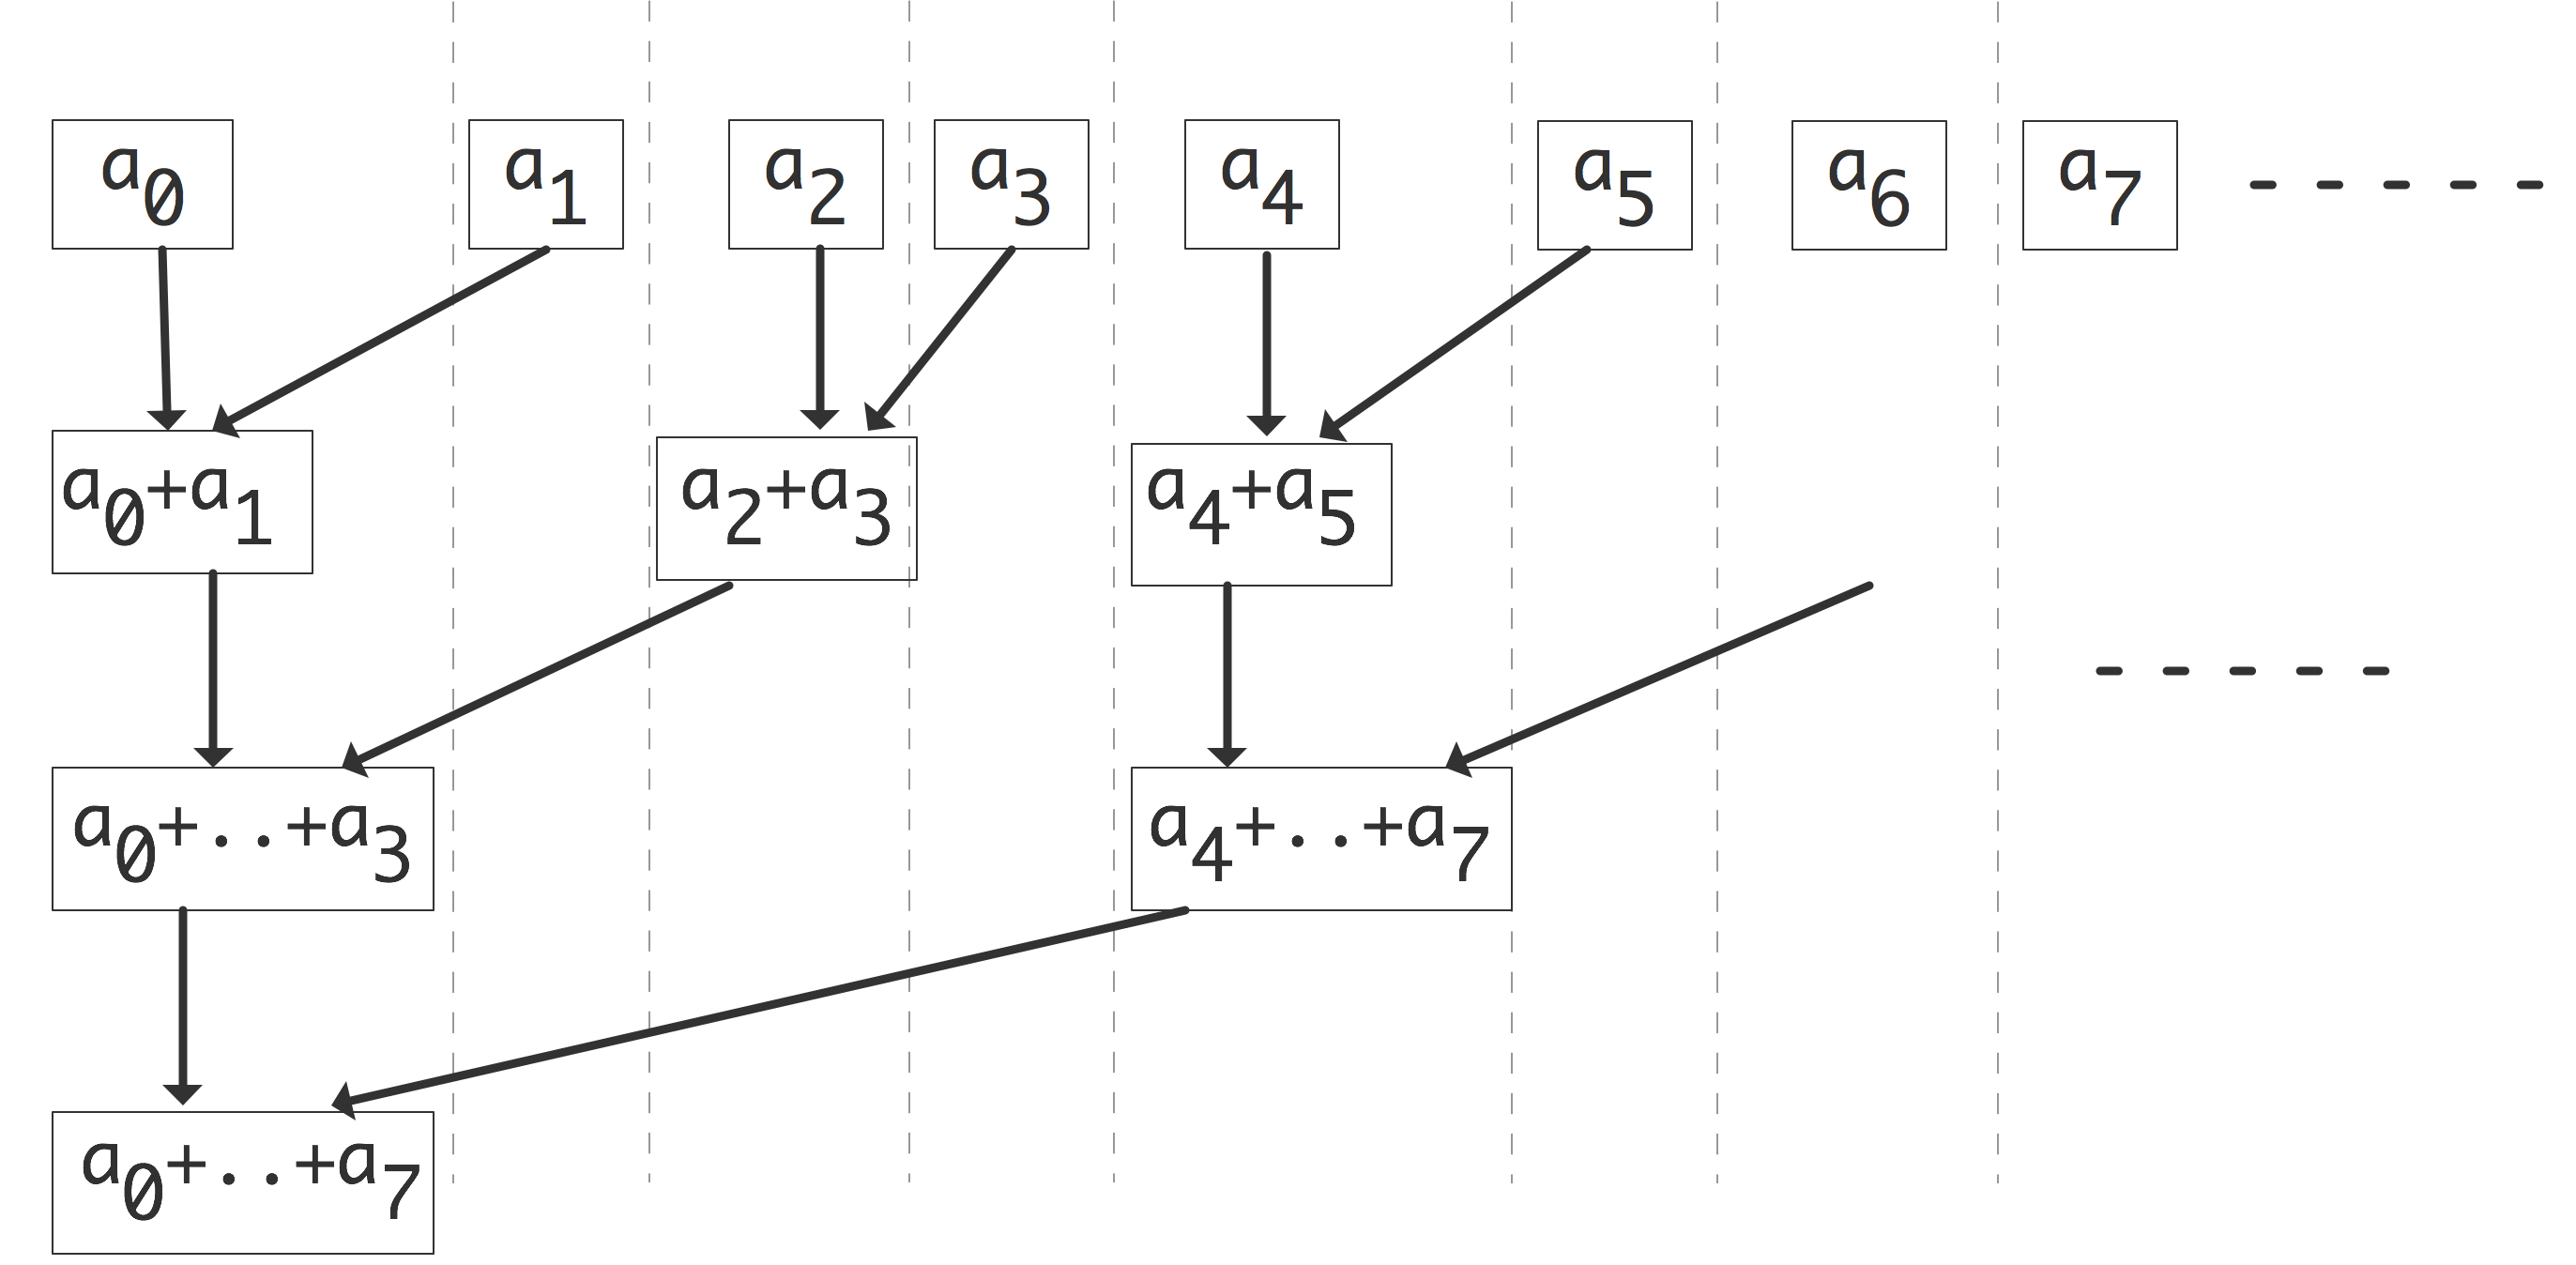
\includegraphics[scale=.13]{graphics/parallel-sum-graph}
  \caption{Communication structure of a parallel vector reduction}
  \label{fig:par-sum-graph}
\end{figure}
The vertical alignment in figure~\ref{fig:par-sum-graph} is not the
only one possible. If nodes are shuffled within a superstep or
horizontal level, a different communication pattern arises.
\begin{exercise}
  Consider placing the nodes within a superstep on random
  processors. Show that, if no two nodes wind up on the same
  processor, at most twice the number of communications is performed
  from the case in figure~\ref{fig:par-sum-graph}.
\end{exercise}

\begin{exercise}
  Can you draw the graph of a computation that leaves the sum result
  on each processor? There is a solution that takes twice the number
  of supersteps, and there is one that takes the same number. In both
  cases the graph is no longer a tree, but a more general \ac{DAG}.
\end{exercise}

Processors are often connected through a network, and moving data
through this network takes time. This introduces a concept of distance
between the processors. This is easily see in figure~\ref{fig:par-sum-graph}
where the
processors are linearly ordered. If the network only connects a
processor with its immediate neighbours,  each iteration of the
outer loop increases the distance over which communication takes
place.

\begin{exercise}
  \label{ex:summing0}
  Assume that an addition takes a certain unit time, and that moving a
  number from one processor to another takes that same unit time. Show
  that the communication time equals the computation time.

  Now assume that sending a number from processor $p$ to $p\pm k$
  takes time~$k$. Show that the execution time of the parallel
  algorithm now is of the same order as the sequential time.
\end{exercise}

The summing example made the unrealistic assumption that every
processor initially stored just one vector element: in practice we will
have $p<n$, and every processor stores a number of vector
elements. The obvious strategy is to give each processor a consecutive
stretch of elements, but sometimes the obvious strategy is not the
best.

\begin{exercise}
  Consider the case of summing 8 elements with 4 processors. Show that
  some of the edges in the graph of figure~\ref{fig:par-sum-graph} no
  longer correspond to actual communications. 
  %
  Now consider summing 16 elements with, again, 4 processors. What is
  the number of communication edges this time?
\end{exercise}

These matters of algorithm adaptation, efficiency, and communication,
are crucial to all of parallel computing. We will return to these
issues in various guises throughout this chapter.

\Level 1 {Functional parallelism versus data parallelism}

From the above introduction we can describe parallelism as finding
independent operations in the execution of a program. In all of the examples
these independent operations were in fact identical operations, but applied to
different data items. We could call this\indexterm{data parallelism}: the same
operation is applied in parallel to many data elements.
This is in fact a common scenario in scientific computing: parallelism
often stems from the fact that a data set (vector, matrix,
graph,\ldots) is spread over many processors, each working on its part
of the data. 

The term data parallelism is traditionally mostly applied
if the operation is a single instruction; in the case of a subprogram
it is often called \indexterm{task parallelism}.

It is also possible to find independence, not based on data elements,
but based on the instructions themselves. Traditionally, compilers
analyze code in terms of \ac{ILP}: independent instructions can be given
to separate floating point units, or reordered, for instance to optimize
register usage (see also section~\ref{sec:ILP}).
\ac{ILP} is one case of \indexterm{functional parallelism};
on a higher level, functional parallelism can be obtained
by considering independent subprograms, often called \indexterm{task parallelism};
see section~\ref{sec:task-parallel}.

Some examples of functional parallelism are Monte Carlo simulations,
and other algorithms that traverse a parametrized search space,
such as boolean \indexterm{satisfyability} problems.

\Level 1 {Parallelism in the algorithm versus in the code}

Often we are in the situation that we want to parallelize an algorithm
that has a common expression in sequential form. In some cases, this
sequential form can easily be parallelized, such as in the vector
addition discussed above. In other cases there is no simple way to
parallelize the algorithm; we will discuss linear recurrences in
section~\ref{sec:recdouble}. And in yet another case the sequential code may
look not parallel, but the algorithm actually has parallelism.

\begin{exercise}
\begin{verbatim}
for i in [1:N]:
    x[0,i] = some_function_of(i)
    x[i,0] = some_function_of(i)

for i in [1:N]:
    for j in [1:N]:
        x[i,j] = x[i-1,j]+x[i,j-1]
\end{verbatim}

Answer the following questions about the double \n{i,j} loop:
\begin{enumerate}
\item Are the iterations of the inner loop independent, that is, could
  they be executed simultaneously?
\item Are the iterations of the outer loop independent?
\item If \n{x[1,1]} is known, show that \n{x[2,1]} and \n{x[1,2]} can
  be computed independently.
\item Does this give you an idea for a parallelization strategy?
\end{enumerate}
\end{exercise}

We will discuss the solution to this conundrum in
section~\ref{sec:wavefront}. In general, the whole of
chapter~\ref{ch:parallellinear} will be about the amount of
parallelism intrinsic in scientific computing algorithms.

\Level 0 {Theoretical concepts}
\label{sec:speedup-efficiency}

There are two important reasons for using a parallel computer: to have
access to more memory or to obtain higher performance. It is easy to
characterize the gain in memory, as the total memory is the sum of the
individual memories. The speed of a parallel computer is harder to
characterize. This section will have an extended discussion on
theoretical measures for expressing and judging the gain in execution
speed from going to a parallel architecture.

\Level 1 {Definitions}
\label{sec:speedup}

\Level 2 {Speedup and efficiency}

A~simple approach to defining speedup is to let the same program run on a
single processor, and on a parallel machine with $p$ processors, and
to compare runtimes.
With $T_1$ the execution time on a single processor and
$T_p$ the time on $p$ processors, we define the \indextermdef{speedup} as
$S_p=T_1/T_p$. (Sometimes $T_1$ is defined as `the best time to solve the
problem on a single processor', which allows for using a different
algorithm on a single processor than in parallel.)
In the ideal case, $T_p=T_1/p$, but in practice we don't expect to
attain that, so $S_p\leq p$. To measure how far we are from the ideal
speedup, we introduce the \indextermdef{efficiency} $E_p=S_p/p$. Clearly,
$0< E_p\leq 1$.

There is a practical problem with
the above definitions: a problem that can be solved on a parallel machine
may be too large to fit on any single processor. Conversely,
distributing a single processor problem
over many processors may give a distorted picture since very little
data will wind up on each processor. Below we will discuss more
realistic measures of speed-up.

There are various reasons why the actual speed is less than~$p$. For
one, using more than one processors necessitates communication, which
is overhead that was not part of the original computation. Secondly,
if the processors do not have exactly the same amount of work to do,
they may be idle part of the time (this is known as
\indextermbus{load}{unbalance}), again lowering the actually attained
speedup. Finally, code may have sections that are inherently
sequential.

Communication between processors is an important source of a loss of
efficiency. Clearly, a problem that can be solved without
communication will be very efficient. Such problems, in effect
consisting of a number of completely independent calculations, is
called \indexterm{embarrassingly parallel}; it will have close to a perfect
speedup and efficiency.

\begin{exercise}
  The case of speedup larger than the number of processors is called
  \indexterm{superlinear speedup}. Give a theoretical argument why
  this can never happen.
\end{exercise}

In practice, superlinear speedup can happen. For instance, suppose a 
problem is too large to fit in memory, and a single processor can only
solve it by swapping data to disc. If the same problem fits in the
memory of two processors, the speedup may well be larger than~$2$
since disc swapping no longer occurs. Having less, or more localized,
data may also improve the cache behaviour of a code.

\Level 2 {Cost-optimality}

In cases where the speedup is not perfect we can define
\indexterm{overhead} as the difference \[ T_o = pT_p-T1. \]
We can also interpret this as the difference between simulating the
parallel algorithm on a single processor, and the actual best
sequential algorithm.

We will later see two different types of overhead:
\begin{enumerate}
\item The parallel algorithm can be essentially different from the
  sequential one. For instance, sorting algorithms have a
  complexity~$O(n\log n)$, but the parallel bitonic sort
  (section~\ref{app:bitonicsort}) has complexity~$O(n\log^2n)$.
\item The parallel algorithm can have overhead derived from the
  process or parallelizing, such as the cost of sending messages. As
  an example, section~\ref{sec:densescaling} analyzes the
  communication overhead in the matrix-vector product.
\end{enumerate}

A parallel algorithm is called \indexterm{cost-optimal} if the
overhead is at most of the order of the running time of the sequential
algorithm.

\begin{exercise}
  The definition of overhead above implicitly assumes that overhead is
  not parallelizable. Discuss this assumption in the context of the
  two examples above.
\end{exercise}

\Level 2 {Critical path}
\label{sec:critical-path}

The above definitions of speedup and efficiency made an implicit assumption
that parallel work can be arbitrarily subdivided.
As you saw in the summing example in section~\ref{sec:parallel-intro},
this may not always be the case: there can be dependencies between
operations, which limits the amount of parallelism that can be
employed.

In order to take this into account, we define the following concepts:
\begin{definition}
  \[ 
  \begin{array}{l@{\colon}l}
    T_1&\hbox{the time the computation takes on a single processor}\\
    T_p&\hbox{the time the computation takes with $p$ processors}\\
    T_\infty&\hbox{the time the computation takes if unlimited processors are available}\\
    P_\infty&\hbox{the value of $p$ for which $T_p=T_\infty$}
  \end{array}  
  \]
\end{definition}
With these concepts, we can define the \indextermsub{average}{parallelism}
of an algorithm as $T_1/T_\infty$.

We will now give a few illustrations by showing a graph of tasks and their dependencies.
We assume for simplicity that each node is a unit time task.

\begin{minipage}{\textwidth}
  \begin{minipage}{.25\textwidth}
    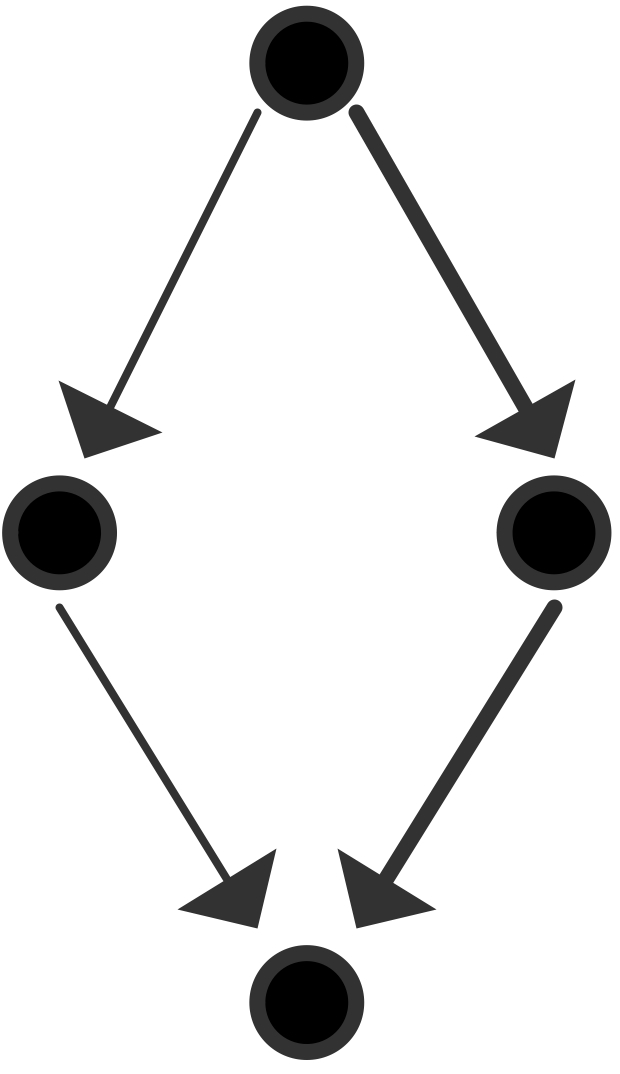
\includegraphics[scale=.07]{critical1}
  \end{minipage}
  \begin{minipage}{.75\textwidth}
    The maximum number of processors that can be used is~2 and the
    average parallelism is~$4/3$:
    \[
    \begin{array}{l}
      T_1=4,\quad T_\infty=3 \quad\Rightarrow T_1/T_\infty=4/3\\
      T_2=3,\quad S_2=4/3,\quad E_2=2/3\\
      P_\infty=2
    \end{array}
    \]
  \end{minipage}
\end{minipage}

\begin{minipage}{\textwidth}
  \begin{minipage}{.25\textwidth}
    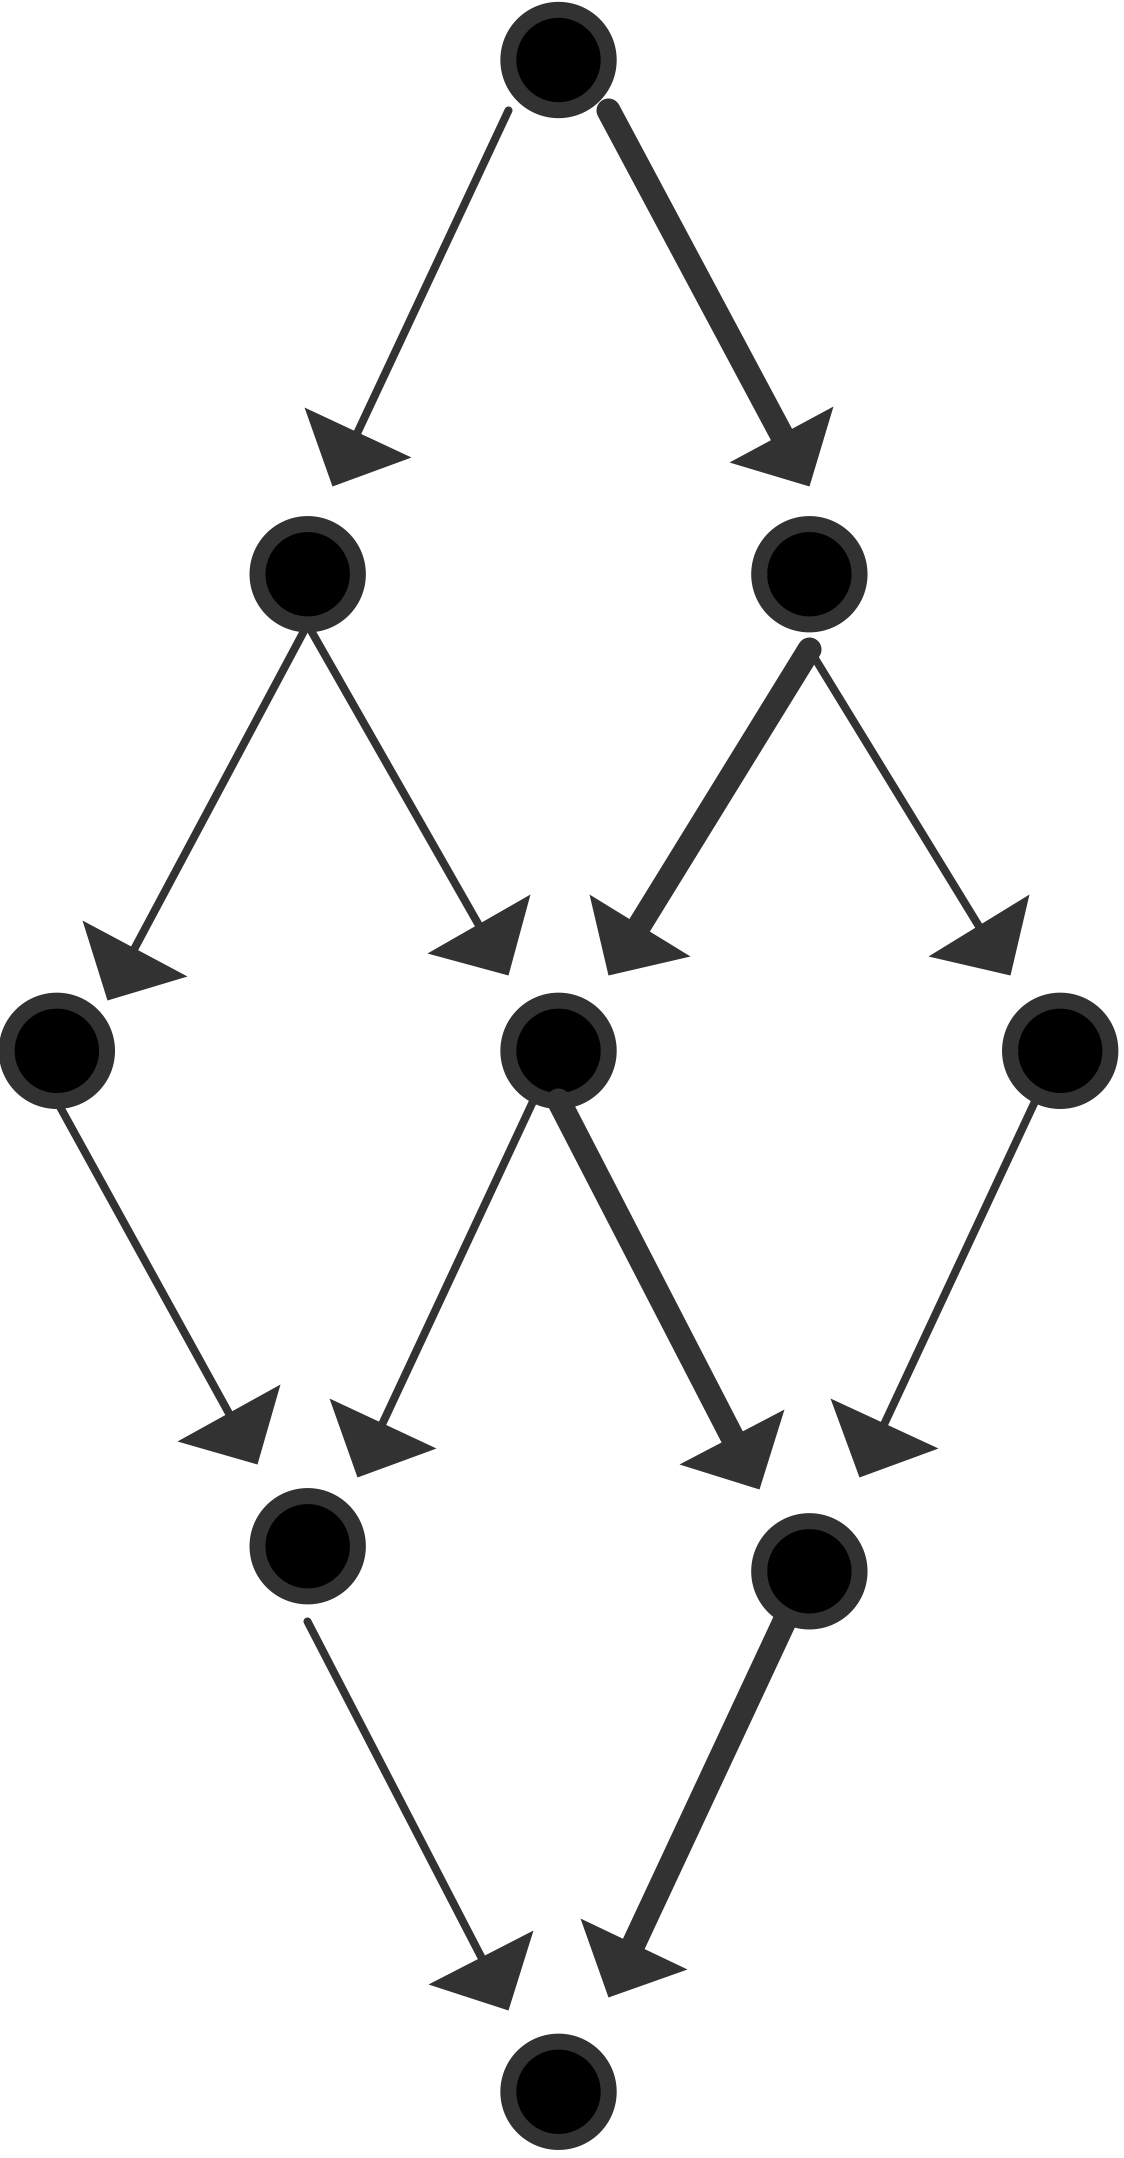
\includegraphics[scale=.07]{critical2}
  \end{minipage}
  \begin{minipage}{.75\textwidth}
    The maximum number of processors that can be used is~3 and the
    average parallelism is~$9/5$; efficiency is maximal for~$p=2$:
    \[
    \begin{array}{l}
      T_1=9,\quad T_\infty=5 \quad\Rightarrow T_1/T_\infty=9/5\\
      T_2=6,\quad S_2=3/2,\quad E_2=3/4\\
      T_3=5,\quad S_3=9/5,\quad E_3=3/5\\
      P_\infty=3
    \end{array}
    \]
  \end{minipage}
\end{minipage}

\begin{minipage}{\textwidth}
  \begin{minipage}{.4\textwidth}
    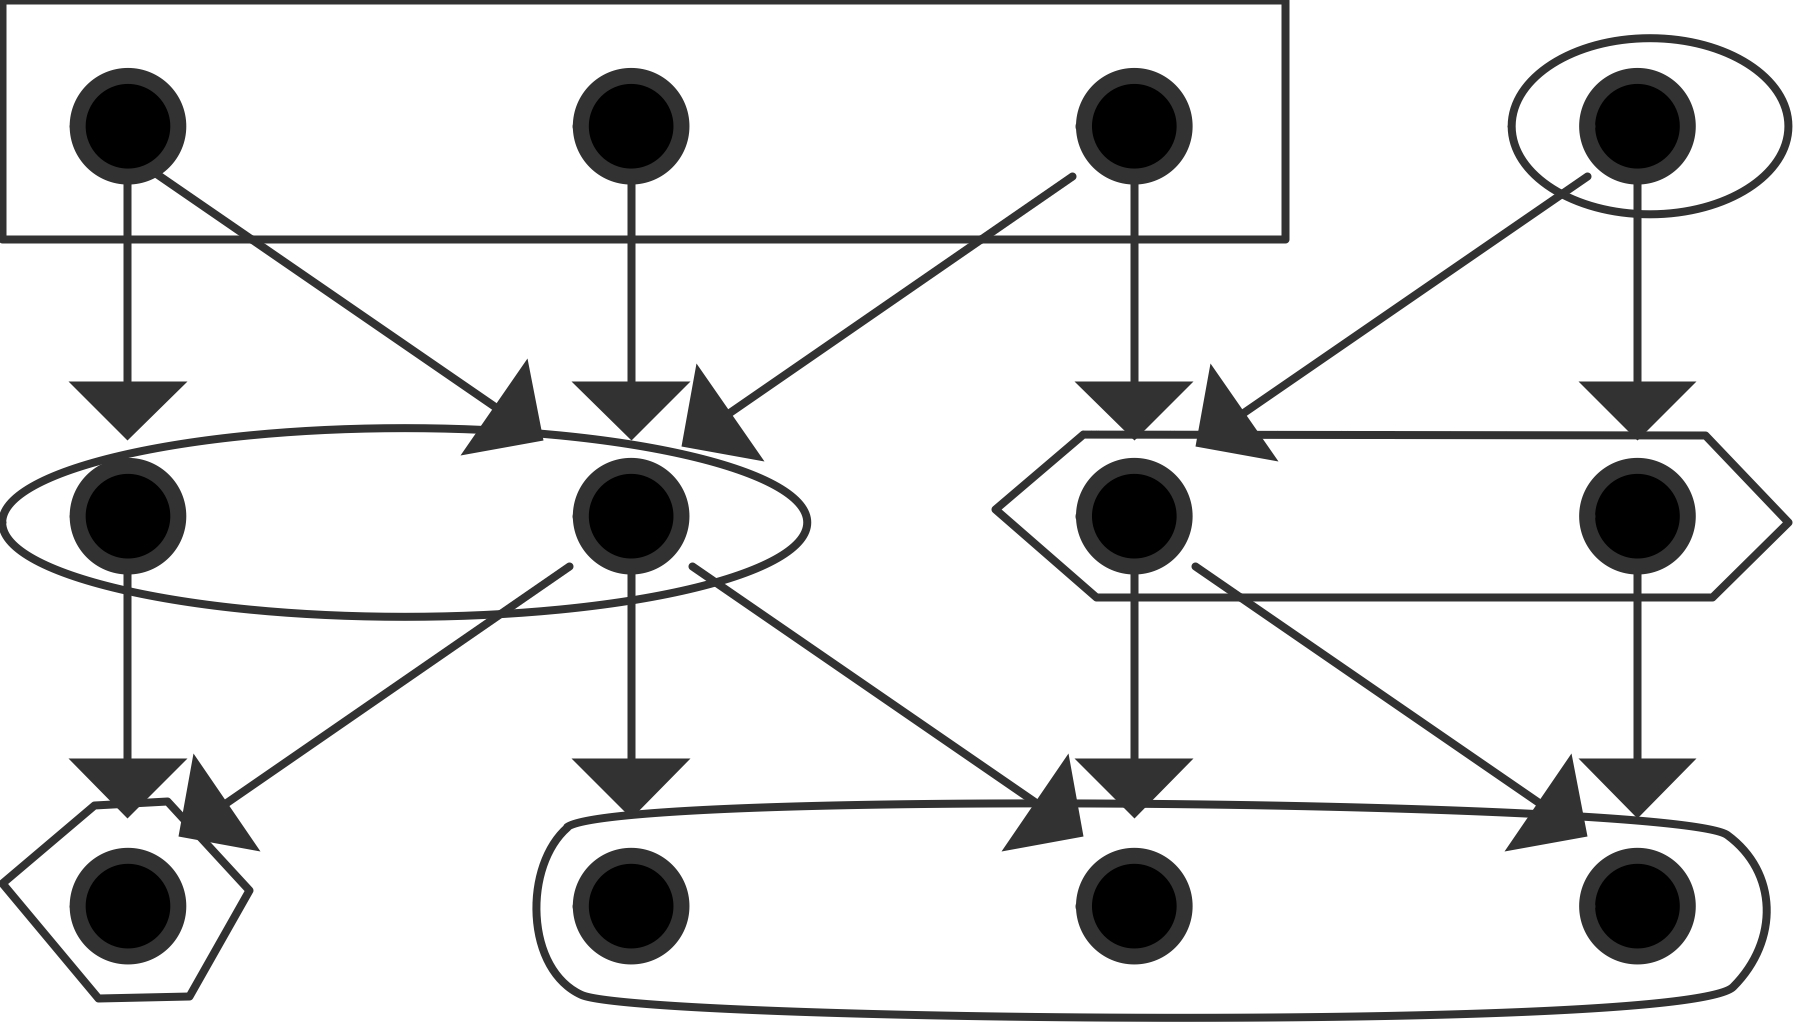
\includegraphics[scale=.07]{critical3}
  \end{minipage}
  \begin{minipage}{.6\textwidth}
    The maximum number of processors that can be used is~4
    and that is also the average parallelism;
    the figure illustrates a parallelization with $P=3$ that
    has efficiency~$\equiv1$:
    \[
    \begin{array}{l}
      T_1=12,\quad T_\infty=4 \quad\Rightarrow T_1/T_\infty=3\\
      T_2=6,\quad S_2=2,\quad E_2=1\\
      T_3=4,\quad S_3=3,\quad E_3=1\\
      T_4=3,\quad S_4=4,\quad E_4=1\\
      P_\infty=4
    \end{array}
    \]
  \end{minipage}
\end{minipage}

Based on these examples, you probably see that there are two extreme cases:
\begin{itemize}
\item If every task depends on precisely on other, you get a chain
  of dependencies, and $T_p=T_1$ for any~$p$.
\item On the other hand, if all tasks are independent (and $p$~divides
  their number) you get $T_p=T_1/p$ for any~$p$.
\item In a slightly less trivial scenario than the previous,
  consider the case where
  the critical path is of length~$m$, and in each of these $m$ steps
  there are $p-1$ independent tasks, or at least: dependent only on
  tasks in the previous step. There will then be perfect parallelism
  in each of the $m$ steps, and we can express $T_p = T_1/p$
  or $T_p= m+ (T_1-m)/p$.
\end{itemize}

That last statement actually holds in general. This is known as
\indextermdef{Brent's theorem}:
\begin{theorem}
  Let $m$ be the total number of tasks, $p$~the number of processors,
  and $t$ the length of a \indexterm{critical path}. Then
  the computation can be done in \[ T_p = t +\frac{m-t}{p}. \]
\end{theorem}
\begin{proof}
  Divide the computation in steps, such that tasks in step~$i+1$
  are independent of each other, and only dependent on step~$i$.
  Let $s_i$ be the number of tasks in step~$i$, then the time
  for that step is $\lceil \frac{s_i}{p} \rceil$.
  Summing over~$i$ gives
  \[ T_p = \sum_i^t \lceil \frac{s_i}{p} \rceil
  \leq \sum_i^t  \frac{s_i+p-1}{p}  = t + \sum_i^t  \frac{s_i-1}{p}  = t+\frac{m-t}{p}.
  \]
\end{proof}

\Level 1 {Asymptotics}
\label{sec:asymptotics}
\input chapters/asymptotics

\Level 1 {Amdahl's law}
\label{sec:amdahl}
\index{Amdahl's law|(}

One reason for less than perfect speedup is that parts of a code can
be inherently sequential. This limits the parallel efficiency as
follows. Suppose that $5\%$ of a code is sequential, then the time for
that part can not be reduced, no matter how many processors are
available. Thus, the speedup on that code is limited to a factor
of~$20$. This phenomenon is known as \emph{Amdahl's
  Law}~\cite{amd:law}, which we will now formulate.

Let $F_s$ be the
\indexterm{sequential fraction} and
$F_p$ be the \indexterm{parallel fraction} 
(or more strictly: the `parallelizable'
fraction) of a code, respectively. Then $F_p+F_s=1$. The parallel
execution time $T_p$ on $p$ processors
is the sum of the part that is sequential
$T_1F_s$ and the part that can be parallelized $T_1F_p/P$:
\begin{equation}
  T_P=T_1(F_s+F_p/P).
  \label{eq:amdahl}
\end{equation}
As the number of processors grows
$P\rightarrow\infty$, the parallel execution time now approaches that
of the sequential fraction of the code: $T_P\downarrow
T_1F_s$. We conclude that speedup is limited by $S_P\leq 1/F_s$ and
efficiency is a decreasing function $E\sim 1/P$.

The sequential fraction of a code can consist of things such as I/O
operations. However, there are also parts of a code that in effect act
as sequential. Consider a program that executes a single loop, where
all iterations can be computed independently. Clearly, this code is
easily parallelized. However, by splitting the loop in a number of
parts, one per processor, each processor now has to deal with loop
overhead: calculation of bounds, and the test for completion. This
overhead is replicated as many times as there are processors. In
effect, loop overhead acts as a sequential part of the code.

\begin{exercise}
  Let's do a specific example. Assume that a code has a setup that
  takes 1~second and a parallelizable section that takes 1000~seconds
  on one processor. What are the speedup and efficiency if the code is
  executed with 100 processors? What are they for 500~processors?
  Express your answer to at most two significant digits.
\end{exercise}

\begin{exercise}
  Investigate the implications of Amdahl's law: if the number of
  processors~$P$ increases, how does the parallel fraction of a code
  have to increase to maintain a fixed efficiency?
\end{exercise}


\Level 2 {Amdahl's law with communication overhead}

In a way, Amdahl's law, sobering as it is, is even optimistic.
Parallelizing a code will give a certain speedup, but it also
introduces \indextermbus{communication}{overhead} that will lower the
speedup attained. Let us refine our model of
equation~\eqref{eq:amdahl} (see~\cite[p.~367]{Landau:comp-phys}):
\[ T_p= T_1(F_s+F_p/P) +T_c, \]
where $T_c$ is a fixed communication time.

To assess the influence of this communication overhead, we assume that
the code is fully parallelizable, that is, $F_p=1$. We then find that
\begin{equation}
    S_p=\frac{T_1}{T_1/p+T_c}.
    \label{eq:amdahl-comm}
\end{equation}
For this to be close to~$p$, we need $T_c\ll T_1/p$ or $p\ll
T_1/T_c$. In other words, the number of processors should not grow
beyond the ratio of scalar execution time and communication overhead.

\Level 2 {Gustafson's law}
\index{Gustafson's law|(}

Amdahl's law was thought to show that large numbers of processors
would never pay off. However, the implicit assumption in Amdahl's law
is that there is a fixed computation which gets executed on more and
more processors. In practice this is not the case: typically there is
a way of scaling up a problem (in chapter~\ref{ch:odepde} you will
learn the concept of `discretization'), and one
tailors the size of the problem to the number of available processors.

A more realistic assumption would be to say that there is a  sequential
fraction independent of the problem size, and parallel fraction that
can be arbitrarily replicated.  To formalize this, instead of starting
with the execution time of the sequential program, let us start with
the execution time of the parallel program, and say that
\[ T_p=T(F_s+F_p) \qquad\hbox{with $F_s+F_p=1$}. \]
Now we have two possible definitions of~$T_1$. First of all, there is the $T_1$ 
you get from setting $p=1$ in~$T_p$. (Convince yourself that that is actually 
the same as~$T_p$.) However, what we need is $T_1$ describing the time
to do all the operations of the parallel program.
This is:
\[ T_1=F_sT+p\cdot F_pT. \]
This gives us a speedup of
\[ S_p=\frac{T_1}{T_p}=\frac{F_s+p\cdot F_p}{F_s+F_p}
   = F_s+p\cdot F_p = p-(p-1)\cdot F_s. 
\]
That is, speedup is now a function that decreases from $p$, linearly
with~$p$.

As with Amdahl's law, we can investigate the behaviour of Gustafson's
law if we include communication overhead. Let's go back to
equation~\eqref{eq:amdahl-comm} for a perfectly parallelizable
problem, and approximate it as
\[ S_p = p(1-\frac{T_c}{T_1}p). \]
Now, under the assumption of a problem that is gradually being scaled up,
$T_c,T_1$ become functions of~$p$. We see that if $T_1(p)\sim pT_c(p)$,
we get linear speedup that is a constant fraction away from~$1$.
In general we can not take this analysis further; in section~\ref{sec:densescaling}
you'll see a detailed analysis of an example. 

\index{Gustafson's law|)}

\Level 2 {Amdahl's law and hybrid programming}

Above, you learned about hybrid programming, a mix between distributed
and shared memory programming. This leads to a new form of Amdahl's
law.

Suppose we have $p$ nodes with $c$ cores each, and $F_p$ describes the fraction
of the code that uses $c$-way thread parallelism. We assume that the
whole code is fully parallel over the $p$ nodes.
The ideal speed up would be $p c$, and the ideal parallel running
time $T_1/(pc)$, but the actual running time is 
\[
  T_{p,c} = T_1 \left(\frac {F_s}{p} + \frac{F_p}{p c}\right)
  = \frac{T_1}{pc}\left( F_sc+F_p\right) 
  = \frac{T_1}{pc}\left( 1+ F_s(c-1)\right).
\]
\begin{exercise}
  Show that the speedup $T_1/T_{p,c}$ can be approximated by~$p/F_s$.
\end{exercise}
In the original Amdahl's law, speedup was limited by the sequential
portion to a fixed number~$1/F_s$, in hybrid programming it is limited
by the task parallel portion to~$p/F_s$.

\index{Amdahl's law|)}

\Level 1 {Scalability}
\label{sec:scaling}
\index{scaling|(}\index{scalability|(}

Above, we remarked that splitting a given problem over more and more
processors does not make sense: at a certain point there is just not
enough work for each processor to operate efficiently. Instead, in
practice, users of a parallel code will either choose the number of
processors to match the problem size, or they will solve a series of
increasingly larger problems on correspondingly growing numbers of
processors. In both cases it is hard to talk about speedup. Instead,
the concept of \indexterm{scalability} is used.

We distinguish two types of scalability. So-called
\indextermsub{strong}{scalability} is in effect the same as speedup,
discussed above. We say that a program shows strong scalability if,
partitioned over more and more processors, it shows perfect or near
perfect speedup, that is, the execution time goes down linearly with
the number of processors. In terms of efficiency we can describe this
as:
\[ \left.
\begin{array}{l}
  N\equiv\mathrm{constant}\\ P\rightarrow\infty
\end{array}
\right\} \Rightarrow E_P\approx\mathrm{constant}
\]
Typically, one encounters statements like `this
problem scales up to 500 processors', meaning that up to 500
processors the speedup will not noticeably decrease from optimal. It
is not necessary for this problem to fit on a single processor: often
a smaller number such as 64 processors is used as the baseline from
which scalability is judged.

More interestingly, \indextermsubdef{weak}{scalability} is a more vaguely
defined term. It describes that, as problem size and number of
processors grow in such a way that the amount of data per processor
stays constant, the execution time
also stays constant.
This measure is somewhat hard to report, since
the relation between the number of operations and the amount of data
can be complicated. If this relation is linear, one could state that
the amount of data per processor is kept constant, and report that parallel
execution time is constant as the number of processors grows.
In terms of efficiency:
\[ \left.
\begin{array}{l}
  N\rightarrow\infty\\ P\rightarrow\infty\\ M=N/P\equiv\mathrm{constant}
\end{array}
\right\} \Rightarrow E_P\approx\mathrm{constant}
\]

\begin{exercise}
  We can formulate strong scaling as a runtime that is inversely
  proportional to the number of processors: \[ t=c/p. \]
  Show that on a log-log plot, that is, you plot the logarithm of the
  runtime against the logarithm of the number of processors,
  you will get a straight line with slope~$-1$.

  Can you suggest a way of dealing with a non-parallelizable
  section, that is, with a runtime $t=c_1+c_2/p$?
\end{exercise}

\begin{exercise}
  Suppose you are investigating the weak scalability of a code.
  After running it for a couple of sizes and corresponding numbers
  of processes, you find that in each case the flop rate is roughly the same.
  Argue that the code is indeed weakly scalable.
\end{exercise}

\begin{exercise}
  In the above discussion we always implicitly compared a sequential 
  algorithm and the parallel form of that same algorithm. However, 
  in section~\ref{sec:speedup} we noted that sometimes speedup is defined
  as a comparison of a parallel algorithm with the \textbf{best} sequential
  algorithm for the same problem. With that in mind, compare a parallel sorting
  algorithm with runtime $(\log n)^2$ (for instance, \indexterm{bitonic sort};
  section~\ref{sec:sorting}) to the best serial algorithm, which has 
  a running time of $n\log n$.

  Show that in the weak scaling case of $n=p$ speedup is $p/\log p$.
  Show that in the strong scaling case speedup is a descending function of~$n$.
\end{exercise}

\Level 2 {Iso-efficiency}
\label{sec:iso-efficiency}

In the definition of \indextermsub{weak}{scalability} above, we stated
that, under some relation between problem size~$N$ and number of
processors~$P$, efficiency will stay constant. We can make this
precise and define the \indextermdef{iso-efficiency curve} as the
relation between $N,P$ that gives constant
efficiency~\cite{Grama:1993:isoefficiency}.

\Level 2 {Precisely \emph{what} is scalable?}

In industry parlance the term `scalability' is sometimes
applied to architectures or whole computer systems:
\begin{quotation}
  A
  scalable computer is a computer designed from a small number of
  basic components, without a single bottleneck component, so that
  the computer can be incrementally expanded over its designed scaling
  range, delivering linear incremental performance for a well-defined
  set of scalable applications.  General-purpose scalable computers
  provide a wide range of processing, memory size, and I/O
  resources.  Scalability is the degree to which performance
  increments of a scalable computer are linear''~\cite{Bell:outlook}.
\end{quotation}
In scientific computing
scalability is a property of an algorithm and the way it is
parallelized on an architecture, in
particular noting the way data is distributed. In
section~\ref{sec:densescaling} you will find an analysis of the
matrix-vector product operation: distributing a matrix by block rows
turns out not to be scalable, but a two-dimensional distribution by
submatrices is.

\Level 1 {Simulation scaling}

In most discussions of weak scaling
we assume that the amount of work and 
the amount of storage are linearly related. This is not always the case; for instance
the operation complexity of a matrix-matrix product is $N^3$ for $N^2$ data.
If you linearly increase the number of processors, the work will go up with a higher power.

A similar effect comes into play if you simulate time-dependent \acp{PDE}\footnote
{This uses concepts from chapter~\ref{ch:odepde}.}.
Here, the total work is a product of the work per time step and the number of 
time steps. These two numbers are related; in section~\ref{sec:fd-ode} you
saw that the time step has a certain minimum size as a function of the 
space discretization. Thus, the number of time steps will go up as the work per
time step goes up.

Rather than investigating scalability from the point of the running
of an algorithm, in this section we will look at the case where the simulated time~$S$
and the running time~$T$ are constant, and we look at how this influences the amount of
memory we need. This corresponds to the following real-life scenario: 
you have a simulation that models a certain amount of real-world time 
in a certain amount of running time; now you buy a bigger computer, and you wonder
what size problem you can solve in the same running time and maintaining
the same simulated time.

Let $m$ be the memory per processor, and $P$ the number of processors, giving:
\[ M=Pm\qquad\hbox{total memory.} \]
If $d$ is the number of space dimensions of the problem, typically 2~or~3,
we get
\[ \Delta x = 1/M^{1/d}\qquad\hbox{grid spacing.} \]
For stability this limits the time step $\Delta t$ to
\[ \Delta t=
\begin{cases}
\Delta x=1\bigm/M^{1/d}&\hbox{hyperbolic case}\\
\Delta x^2=1\bigm/M^{2/d}&\hbox{parabolic case}
\end{cases}
\]
(noting that the hyperbolic case was not discussed in chapter~\ref{ch:odepde}.)
With a simulated time $S$, we find
\[ k=S/\Delta t\qquad \hbox{time steps.} \]
If we assume that the individual time steps are perfectly parallelizable,
that is, we use explicit methods, or implicit methods with optimal solvers,
we find a running time
\[ T=kM/P=\frac{S}{\Delta t}m. \]
Setting $T/S=C$, we find
\[ m=C\Delta t, \]
that is, the amount of memory per processor goes down as we increase the processor
count. (What is the missing step in that last sentence?)

Further analyzing this result, we find
\[ m=C\Delta t = c
\begin{cases}
1\bigm/M^{1/d}&\hbox{hyperbolic case}\\
1\bigm/M^{2/d}&\hbox{parabolic case}
\end{cases}
\]
Substituting $M=Pm$, we find ultimately
\[ m = C
\begin{cases}
1\bigm/P^{1/(d+1)}&\hbox{hyperbolic}\\
1\bigm/P^{2/(d+2)}&\hbox{parabolic}
\end{cases}
\]
that is, the memory per processor that we can use
goes down as a higher power of the number of processors.

\Level 1 {Other scaling measures}

Amdahl's law above was formulated in terms of the execution time on
one processor. In many practical situations this is unrealistic, since
the problems executed in parallel is too large for any single
processor.  Some formula manipulation gives us quantities that are to
an extent equivalent, but that do not rely on this single-processor
number~\cite{Moreland:formalmetrics2015}.

For starters, applying the definition
%
$S_p(n) = \frac{ T_1(n) }{ T_p(n) }$
%
to strong scaling, we observe that $T_1(n)/n$ is the sequential time
per operation, and its inverse $n/T_1(n)$ can be called the sequential
\indextermsub{computational}{rate}, denoted $R_1(n)$. Similarly
defining a `parallel computational rate'
\begin{equation}
  R_p(n) = n/T_p(n)
\end{equation}
we find that
\[ S_p(n) = R_p(n)/R_1(n) \]
In strong scaling $R_1(n)$ will be a constant, so we
make a logarithmic plot of speedup, purely based on measuring~$T_p(n)$.

\index{scaling|)}\index{scalability|)}

\Level 1 {Concurreny; asynchronous and distributed computing}

Even on computers that are not parallel there is a question of the
execution of multiple simultaneous processes. Operating systems
typically have a concept of \indexterm{time slicing}, where all active
process are given command of the \ac{CPU} for a small slice of time in
rotation. In this way, a sequential can emulate a parallel machine; of
course, without the efficiency.

However, time slicing is useful even when not running a parallel
application: \acp{OS} will have independent processes (your editor,
something monitoring your incoming mail, et cetera) that all need to
stay active and run more or less often. The difficulty with such
independent processes arises from the fact that they sometimes need
access to the same resources. The situation where two processes both
need the same two resources, each getting hold of one, is called
\indexterm{deadlock}. A~famous formalization of
\indexterm{resource contention} is
known as the \indexterm{dining philosophers} problem.

The field that studies such as independent processes is variously
known as
\indextermdef{concurrency},
\indexterm{asynchronous computing}, or
\indexterm{distributed computing}.
The term concurrency describes that we are dealing with tasks that are
simultaneously active, with no temporal ordering between their actions.
The term distributed computing derives from
such applications as database systems, where multiple independent clients need to
access a shared database. 

We will not discuss this topic much in this
book. Section~\ref{sec:threads} discusses the \indexterm{thread}
mechanism that supports time slicing; on modern multicore processors
threads can be used to implement shared memory parallel computing.

The book `Communicating Sequential
Processes' offers an analysis of the interaction between
concurrent processes~\cite{Hoare:CSP}. Other authors use topology to analyze
asynchronous computing~\cite{Herlihy:1999:topological}.

\Level 0 {Parallel Computers Architectures}

For quite a while now, the top computers have been
some sort of parallel computer, that is, an architecture that allows
the simultaneous execution of multiple instructions or instruction
sequences. One way of characterizing the various forms this can take
is due to Flynn~\cite{flynn:taxonomy}. \indexterm{Flynn's taxonomy} 
characterizes architectures by whether the \indexterm{data flow}
and \indexterm{control flow} are shared or independent.
The following four types result (see also figure~\ref{fig:flynn}):
\begin{figure}[t]
  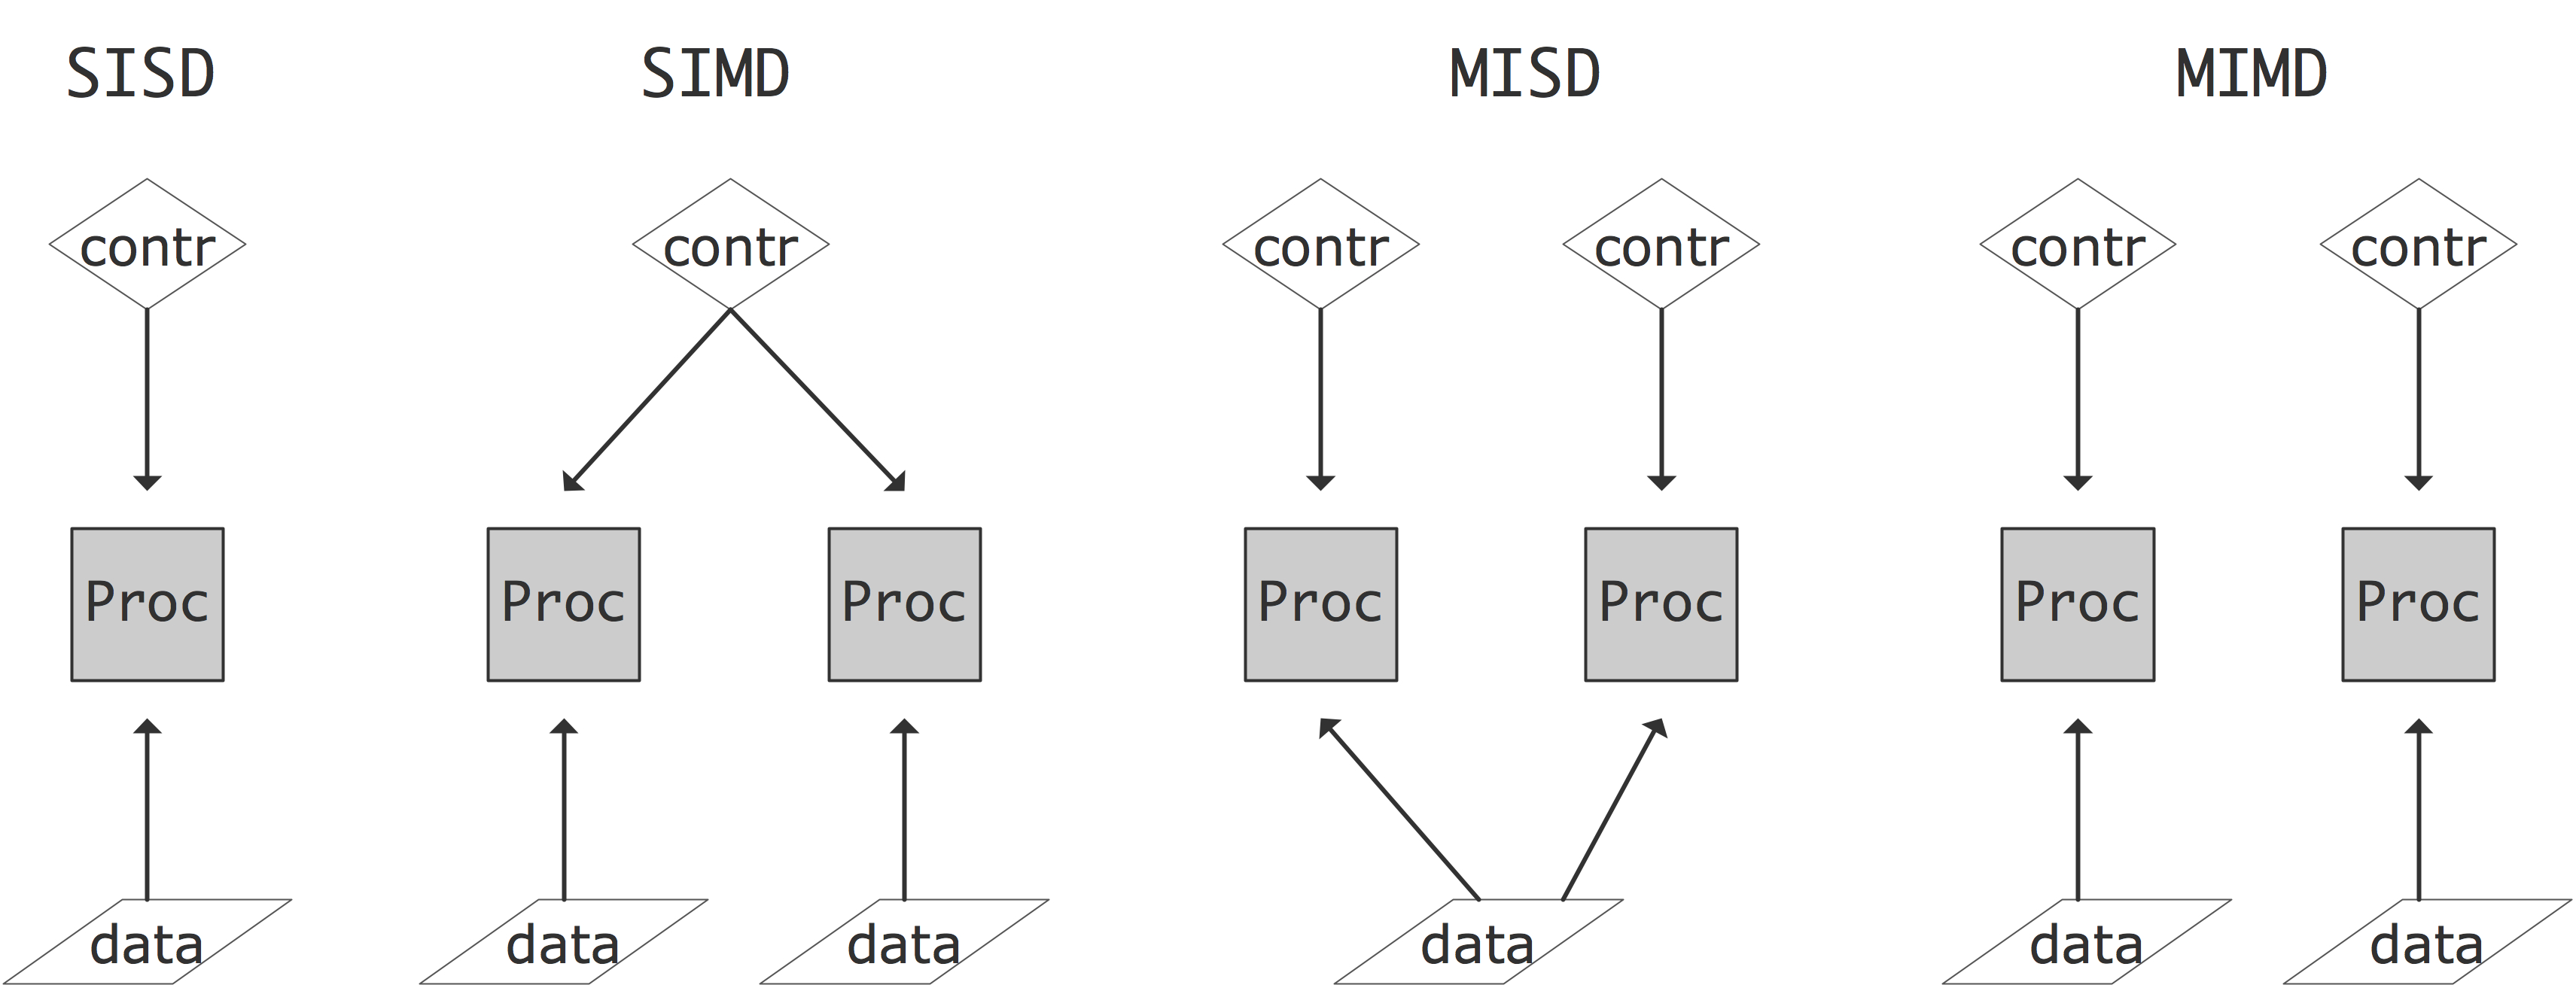
\includegraphics[scale=.12]{Flynn}
  \caption{The four classes of the Flynn's taxonomy}
  \label{fig:flynn}
\end{figure}
\begin{description}
\item[SISD] Single Instruction Single Data: this is the traditional
  CPU architecture: at any one time only a single instruction is
  executed, operating on a single data item.
\item[SIMD] Single Instruction Multiple Data: in this computer type
  there can be multiple processors, each operating on its own data
  item, but they are all executing the same instruction on that data
  item. Vector computers (section~\ref{sec:vector}) are typically also
  characterized as SIMD.
\item[MISD] Multiple Instruction Single Data. No architectures
  answering to this description exist; one could argue that
  redundant computations for safety-critical applications are an
  example of MISD.
\item[MIMD] Multiple Instruction Multiple Data: here multiple CPUs
  operate on multiple data items, each executing independent
  instructions. Most current parallel computers are of this
  type.
\end{description}

We will now discuss SIMD and MIMD architectures in more detail.

\Level 1 {SIMD}
\label{sec:simd}

\begin{lulu}
  \begin{wrapfigure}{r}{2in}
    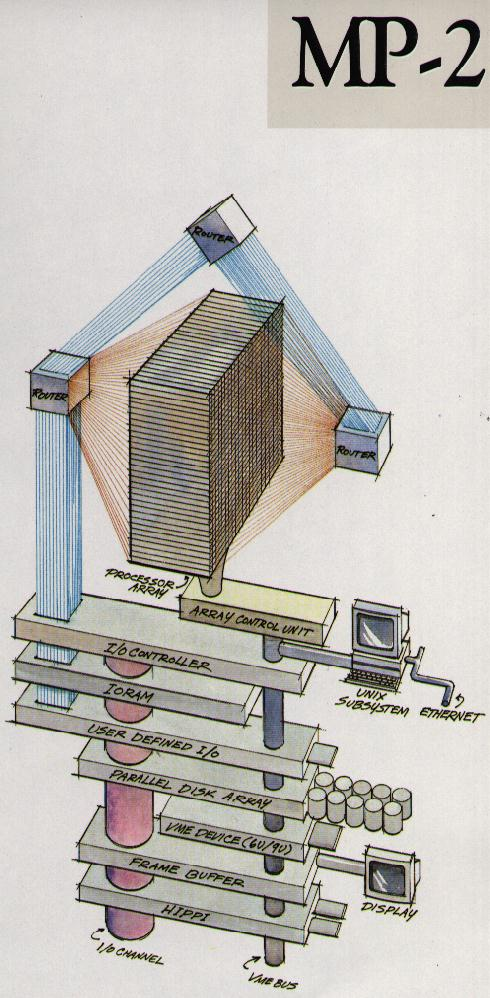
\includegraphics[scale=.3]{maspar2}
    \caption{Architecture of the MasPar 2 array processors}
    \label{fig:maspar}
    %\vskip-1.5in
  \end{wrapfigure}
\end{lulu}
%
Parallel computers of the SIMD type apply the same operation
simultaneously to a number of data items. The design of the CPUs of
such a computer can be quite simple, since the arithmetic unit does
not need separate logic and instruction decoding units: all CPUs
execute the same operation in lock step. 
This makes SIMD computers excel at operations on arrays, such as
%
\begin{verbatim}
for (i=0; i<N; i++) a[i] = b[i]+c[i];
\end{verbatim}
and, for this reason, they are also often called \indexterm{array
  processors}. Scientific codes can often be written so that
a large fraction of the time is spent in array operations.

On the other hand, there are operations that can not can be executed
efficiently on an array processor. For instance, evaluating a number
of terms of a recurrence $x_{i+1}=ax_i+b_i$ involves that many
additions and multiplications, but they alternate, so only one
operation of each type can be processed at any one time. There are no
arrays of numbers here that are simultaneously the input of an
addition or multiplication.

In order to allow for different instruction streams on
different parts of the data, the processor would have a `mask bit'
that could be set to prevent execution of instructions. In code, this 
typically looks like
\begin{verbatim}
where (x>0) {
  x[i] = sqrt(x[i])
\end{verbatim}
The programming model where identical operations are applied to a
number of data items simultaneously, is known as
\indextermsub{data}{parallelism}.

\begin{notlulu}
  \begin{wrapfigure}{r}{2in}
    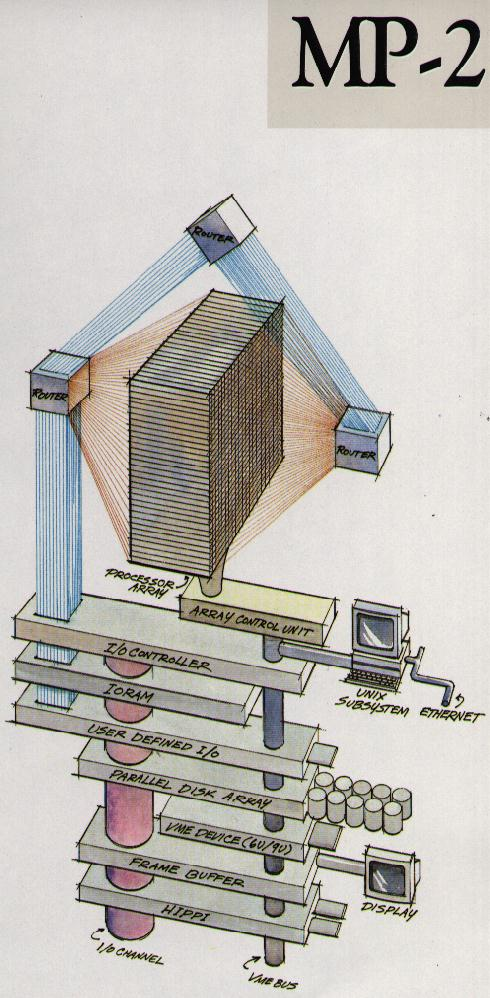
\includegraphics[scale=.3]{maspar2}
    \caption{Architecture of the MasPar 2 array processors}
    \label{fig:maspar}
    %\vskip-1.5in
  \end{wrapfigure}
\end{notlulu}
  %
Such array operations can occur in the context of physics simulations,
but another important source is graphics applications. For this
application, the processors in an array processor can be much weaker
than the processor in a PC: often they are in fact bit processors,
capable of operating on only a single bit at a time. Along these
lines, \emph{ICL}\index{ICL!DAP} had the 4096 processor
DAP~\cite{DAP:79a} in the 1980s, and
\emph{Goodyear}\index{Goodyear!MPP} built a 16K processor
MPP~\cite{Batcher:85a} in the 1970s.

Later, the \indexterm{Connection Machine} (CM-1, CM-2, CM-5) were quite popular.
While the first Connection Machine had bit processors (16 to a chip),
the later models had traditional processors capable of floating point
arithmetic, and were not true SIMD architectures. All were based on a
hyper-cube interconnection network; see section~\ref{sec:hypercube}. Another
manufacturer that had a commercially successful array processor was
\indexterm{MasPar}; figure~\ref{fig:maspar} illustrates the architecture.
You clearly see the single control unit for a square array of processors,
plus a network for doing global operations.

Supercomputers based on array processing do not exist anymore, but the
notion of SIMD lives on in various guises. For instance, \acp{GPU}
are SIMD-based, enforced through their \indexterm{CUDA}
programming language. Also, the \indextermbus{Intel}{Xeon Phi} has a
strong SIMD component. While early SIMD architectures were motivated
by minimizing the number of transistors necessary, these modern
co-processors are motivated by \indextermbus{power}{efficiency}
considerations. Processing instructions (known as
\indextermbus{instruction}{issue}) is actually expensive compared to a
floating point operation, in time, energy, and chip real estate needed.
Using SIMD is then a way to economize on the last two measures.

\Level 2 {Pipelining}
\label{sec:vector}
\index{vector!pipeline|see{pipeline, processor}}

A number of computers have been based on a \indexterm{vector
  processor} or \indextermbus{pipeline}{processor} design. The first
commercially successful supercomputers, the Cray-1 and the Cyber-205
were of this type. In recent times, the Cray-X1 and the NEC SX series
have featured vector pipes. The `Earth Simulator'
computer~\cite{Sato2004}, which led the TOP500
(section~\ref{sec:top500}) for 3~years, was based on NEC~SX
processors.  The general idea behind pipelining was described in
section~\ref{sec:pipeline}.

While supercomputers based on pipeline processors are in a distinct
minority, pipelining is now mainstream in the superscalar CPUs that
are the basis for \indexterm{clusters}. A~typical CPU has pipelined floating point
units, often with separate units for addition and multiplication; see
section~\ref{sec:pipeline}.

However, there are some important differences between pipelining in a
modern superscalar CPU and in, more old-fashioned, vector units.  The
pipeline units in these vector computers are not integrated floating
point units in the CPU, but can better be considered as attached
vector units to a CPU that itself has a floating point unit. The
vector unit has \index{register!vector}\emph{vector registers}\footnote
{The Cyber205 was an exception, with direct-to-memory architecture.}
with a typical
length of 64 floating point numbers; there is typically no `vector
cache'. The logic in vector units is also simpler, often addressable
by explicit vector instructions. Superscalar CPUs, on the other hand,
are fully integrated in the CPU and geared towards exploiting data
streams in unstructured code.

\Level 2 {True SIMD in CPUs and GPUs}
\label{sec:sse-avx}
\index{vector!register|see{register, vector}}

True SIMD array processing can be found in modern CPUs and GPUs, in
both cases inspired by the parallelism that is needed in graphics
applications.

Modern CPUs from Intel\index{Intel} and AMD\index{AMD}, as well as
PowerPC\index{PowerPC} chips, have \indextermbusdef{vector}{instructions} that can perform
multiple instances of an operation simultaneously. On Intel processors
this is known as \indexacf{SSE} or \indexacf{AVX}. These extensions were
originally intended for graphics processing, where often the same
operation needs to be performed on a large number of pixels. Often,
the data has to be a total of, say, 128 bits, and this can be divided
into two 64-bit reals, four~32-bit reals, or a larger number of even
smaller chunks such as 4~bits. 

The \ac{AVX} instructions are based on up to
512-bit wide SIMD, that is, eight floating point numbers can be
processed simultaneously. Just as single floating point operations
operate on data in registers (section~\ref{sec:register}),
vector operations use \index{register!vector|(textbf}\emph{vector registers}.
The locations in a vector register are sometimes referred to as \indextermbusdef{SIMD}{lanes}.

The use of SIMD is mostly
motivated by power considerations. Decoding instructions is actually
more power consuming than executing them, so SIMD parallelism is a way
to save power.

Current compilers can generate \ac{SSE} or \ac{AVX}
instructions automatically;
sometimes it is also possible for the user to insert pragmas, for
instance with the Intel compiler:
\begin{verbatim}
void func(float *restrict c, float *restrict a,
          float *restrict b, int n)
{
#pragma vector always
  for (int i=0; i<n; i++)
    c[i] = a[i] * b[i];
}
\end{verbatim}
Use of these extensions often requires data to be aligned with cache
line boundaries (section~\ref{sec:cacheline}), so there are special
allocate and free calls that return aligned memory.

Version 4 of \emph{OpenMP}\index{OpenMP!version 4} also has directives for indicating SIMD parallelism.

\begin{comment}
For a nontrivial example, see figure~\ref{fig:SSEcomplexmult}, which
describes complex multiplication using SSE3.
\begin{figure}[ht]
  \begin{quote}
  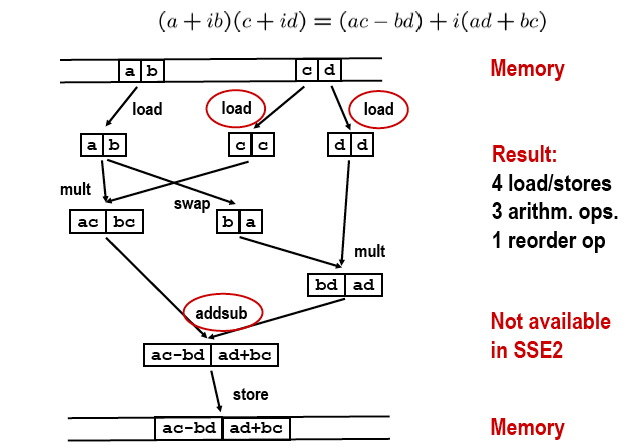
\includegraphics[scale=.5]{graphics/complexmult}
  \end{quote}
  \caption{Complex multiplication with SSE3}
  \label{fig:SSEcomplexmult}
\end{figure}
\end{comment}

Array processing on a larger scale can be found in
\indexac{GPU}s. A~\ac{GPU} contains a large number of simple
processors, ordered in groups of~32, typically. Each processor group
is limited to executing the same instruction. Thus, this is true
example of~\ac{SIMD} processing.
For further discussion, see section~\ref{sec:gpu}.

\Level 1 {MIMD / SPMD computers}
\label{sec:mimd}\label{sec:spmd}
\indexacstart{MIMD}

By far the most common parallel computer architecture these days is
called \acf{MIMD}: the processors execute multiple, possibly differing
instructions, each on their own data. Saying that the instructions
differ does not mean that the processors actually run different
programs: most of these machines operate in \indexacf{SPMD} mode, where the
programmer starts up the same executable on the parallel processors.
Since the different instances of the executable can take differing
paths through conditional statements, or execute differing numbers of
iterations of loops, they will in general not be completely in sync as
they were on \ac{SIMD} machines. If this lack of synchronization is
due to processors working on different amounts of data, it is
called \indextermbus{load}{unbalance}, and it is a major source of less
than perfect \indexterm{speedup}; see section~\ref{sec:load}.

There is a great variety in \ac{MIMD} computers. Some of the aspects
concern the way memory is organized, and the network that connects the
processors. Apart from these hardware aspects, there are also
differing ways of programming these machines. We will see all these
aspects below. Many machines these days are 
called \indexterm{clusters}. They can be built out of custom or
commodity processors (if they consist of PCs, running Linux, and
connected with \indexterm{Ethernet}, they are referred to as \indextermsub{Beowulf}
{clusters}~\cite{Gropp:BeowulfBook}); since the processors are
independent they are examples of the \ac{MIMD} or \ac{SPMD} model.

\indexacend{MIMD}

\Level 1 {The commoditization of supercomputers}
\label{sec:commodity}

In the 1980s and 1990s supercomputers were radically different from
personal computer and mini or super-mini computers such as the DEC PDP
and VAX series. The SIMD vector computers had one
(\indextermbus{CDC}{Cyber205} or \emph{Cray-1}\index{Cray!Cray-1}), or
at most a few (\indexterm{ETA-10}, \emph{Cray-2}\index{Cray!Cray-2},
\indextermbus{Cray}{X/MP}, \indextermbus{Cray}{Y/MP}), extremely
powerful processors, often a vector processor. Around the mid-1990s
clusters with thousands of simpler (micro) processors started taking
over from the machines with relative small numbers of vector pipes
(see \url{http://www.top500.org/lists/1994/11}). At first these
microprocessors (\indextermbus{IBM}{Power series},
\indextermbus{Intel}{i860}, \indexterm{MIPS},
\indextermbus{DEC}{Alpha}) were still much more powerful than `home
computer' processors, but later this distinction also faded to an
extent. Currently, many of the most powerful clusters are powered by
essentially the same Intel Xeon and AMD Opteron chips that are
available on the consumer market. Others use IBM Power Series or other
`server' chips. See section~\ref{sec:top500} for illustrations of
this history since 1993.

\Level 0 {Different types of memory access}

In the introduction we defined a parallel computer as a setup where
multiple processors work together on the same problem. In all but the
simplest cases this means that these processors need access to a joint
pool of data. In the previous chapter you saw how, even on a single
processor, memory can have a hard time keeping up with processor demands.
For parallel machines, where potentially several processors
want to access the same memory location, this problem becomes even
worse. We can characterize parallel machines by the approach they take
to the problem of reconciling multiple accesses, by multiple
processes, to a joint pool of data.

The main distinction here is between
\indextermsub{distributed}{memory} and
\indextermsub{shared}{memory}. With distributed memory, each processor
has its own physical memory, and more importantly its own
\indexterm{address space}.
\begin{figure}
  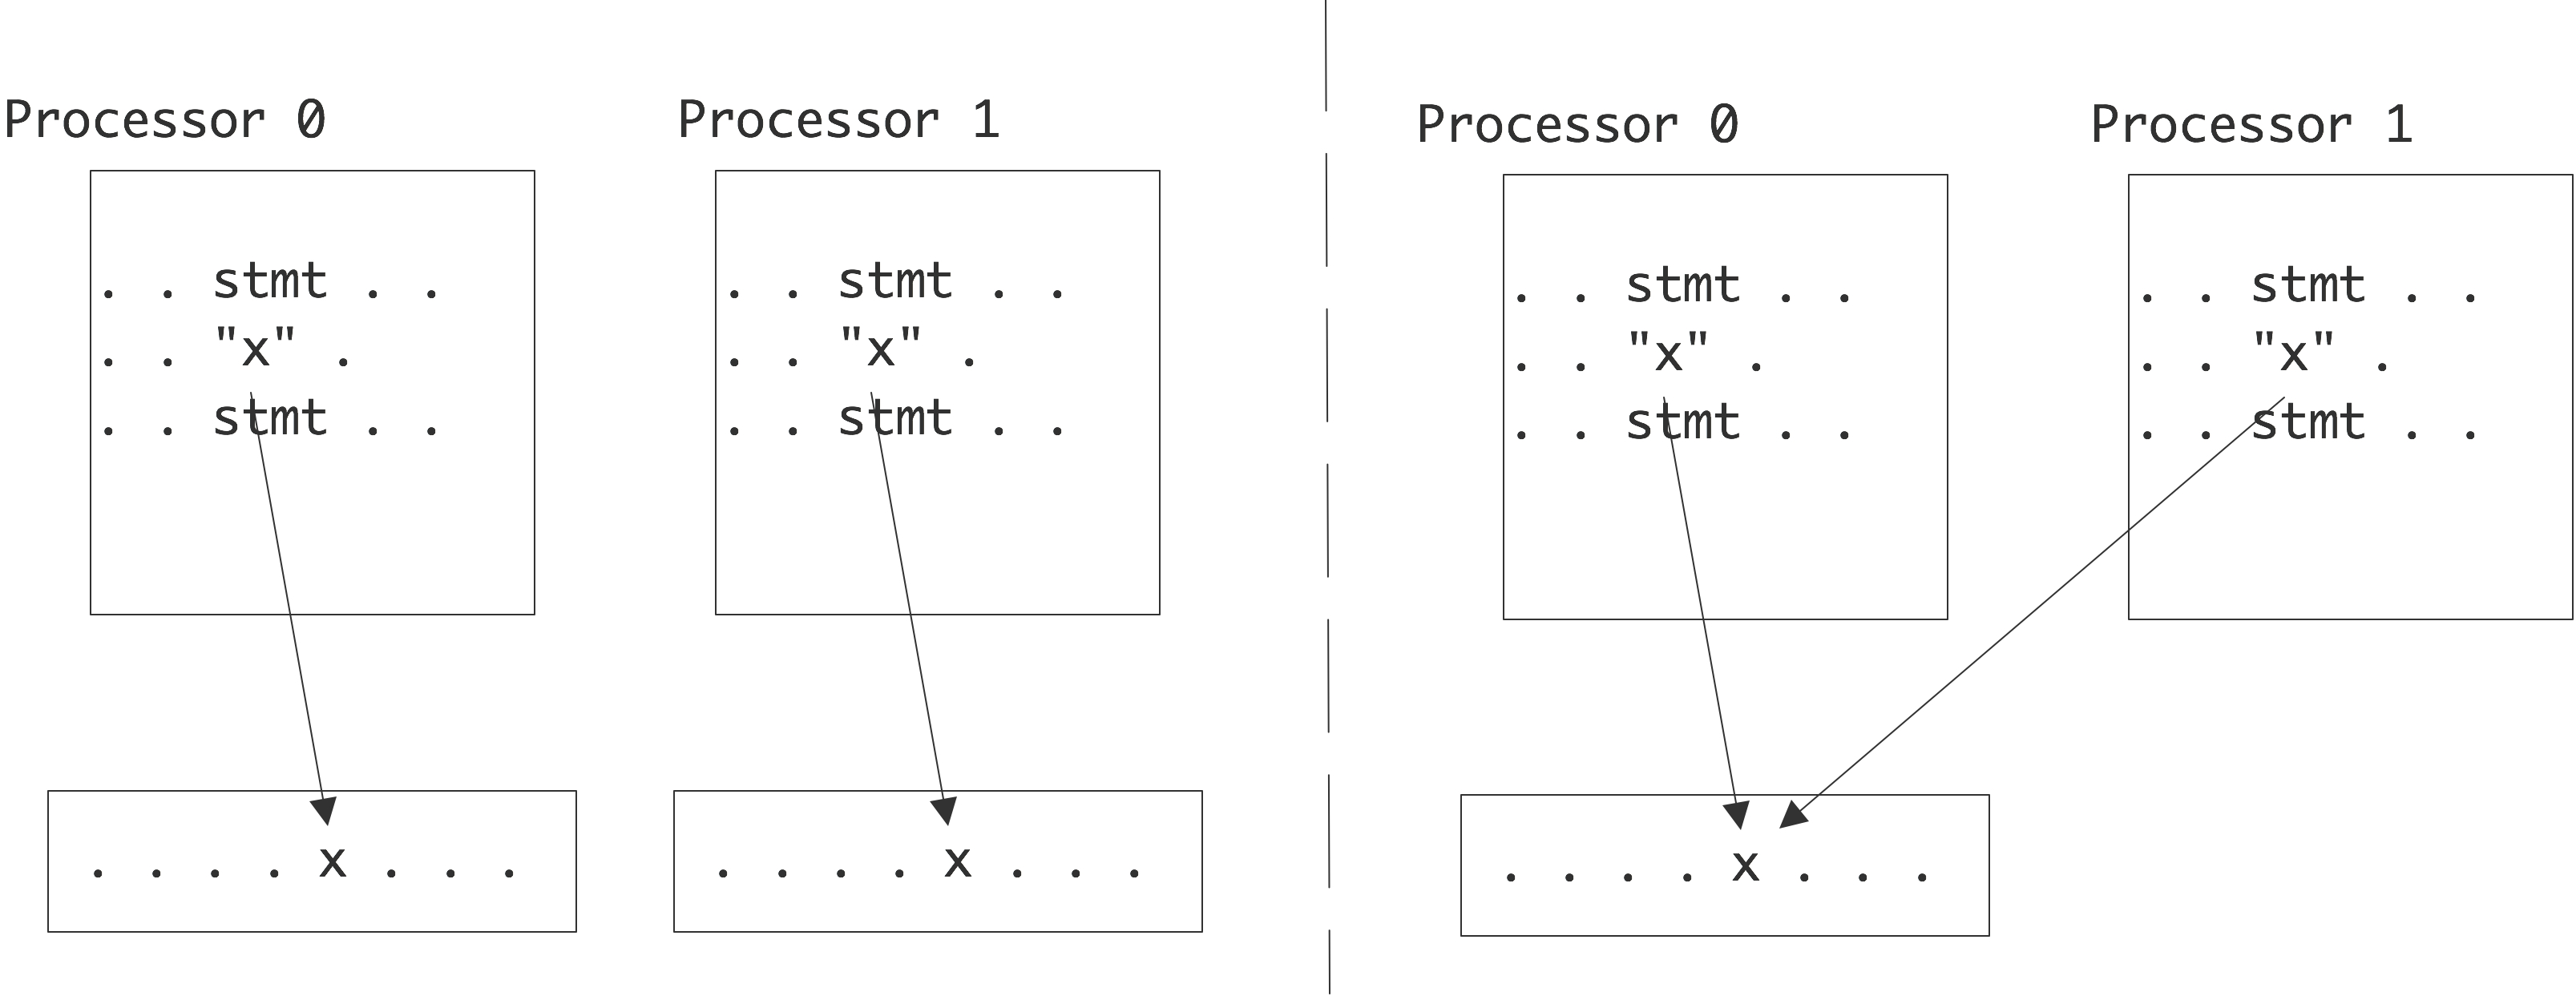
\includegraphics[scale=.1]{graphics/shared-distributed}
  \caption{References to identically named variables in the
    distributed and shared memory case}
  \label{fig:shared-distributed}
\end{figure}
Thus, if two processors refer to a variable~\n{x}, they access a
variable in their own local memory. On the other hand, with shared
memory, all processors access the same memory; we also say that they
have a \indextermsub{shared}{address space}. Thus, if two processors
both refer to a variable~\n{x}, they access the same memory location.

\Level 1 {Symmetric Multi-Processors: Uniform Memory Access}
\label{sec:uma}

Parallel programming is fairly simple if any processor can access any
memory location. For this reason, there is a strong incentive for
manufacturers to make architectures where processors see no difference
between one memory location and another: any memory location is
accessible to every processor, and
the access times do not differ. This is called \indexac{UMA}, and 
the programming model for
architectures on this principle is often called \indexac{SMP}.

There are a few ways to realize an SMP architecture.  Current desktop
computers can have a few processors accessing a shared memory through
a single memory bus; for instance Apple markets a model with 2
six-core processors. Having a memory bus that is shared between
processors works only for small numbers of processors; for larger
numbers one can use a \indexterm{crossbar} that connects multiple
processors to multiple memory banks; see section~\ref{sec:crossbar}.
%%  Figure~\ref{fig:crossbar} shows
%% the simplest type of crossbar, while figure~\ref{fig:butterfly} show
%% the \indexterm{butterfly exchange}, which is built up out of simple
%% elements.

On \indexterm{multicore} processors there is uniform memory access of
a different type: the cores typically have a
\indextermsub{shared}{cache}, typically the L3 or L2 cache.

\Level 1 {Non-Uniform Memory Access}
\label{sec:numa}

The \ac{UMA} approach based on shared memory 
is obviously limited to a small number of
processors. The crossbar networks are expandable, so they would seem 
the best choice. 
However, in practice one puts 
processors with a local memory in a configuration with an exchange
network. This leads to a situation where a processor can access its
own memory fast, and other processors' memory slower.
This is one case of so-called \indexac{NUMA}: a strategy that
uses physically distributed memory, abandoning the uniform access
time, but maintaining the logically shared address space: each processor can
still access any memory location.

\begin{figure}
  \begin{quote}
  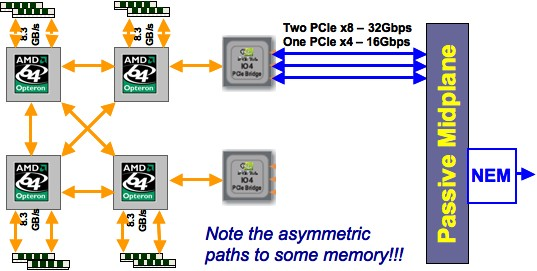
\includegraphics[scale=.6]{graphics/ranger-numa}
  \end{quote}
  \caption{Non-uniform memory access in a four-socket motherboard}
  \label{fig:ranger-numa}
\end{figure}

Figure~\ref{fig:ranger-numa} illustrates \ac{NUMA} in the case of the
four-socket motherboard of the Ranger supercomputer. Each chip has its
own memory (8Gb) but the motherboard acts as if the processors have
access to a shared pool of 32Gb. Obviously, accessing the memory of
another processor is slower than accessing local memory. In addition,
note that each processor has three connections that could be used to
access other memory, but the rightmost two chips use one connection to
connect to the network. This means that accessing each other's memory
can only happen through an intermediate processor, slowing down the
transfer, and tying up that processor's connections.

While the \ac{NUMA} approach is convenient for the programmer, it offers some
challenges for the system. Imagine that two different processors each
have a copy of a memory location in their local (cache) memory. If one
processor alters the content of this location, this change has to be
propagated to the other processors. If both processors try to alter
the content of the one memory location, the behaviour of the program
can become undetermined.

Keeping copies of a memory location synchronized is known as
\indextermbus{cache}{coherence} (see section~\ref{sec:coherence} for further details);
a multi-processor system using it is sometimes called a
`cache-coherent NUMA' or \indexterm{ccNUMA} architecture.

Taking NUMA to its extreme, it is possible to have a software layer
that makes network-connected processors appear to operate on shared memory.
This is known as \indextermsub{distributed shared}{memory} 
or \indextermsub{virtual shared}{memory}. In this approach
a \indexterm{hypervisor} offers a shared memory API, by translating
system calls to distributed memory management. This shared memory 
API can be utilized by the \indextermbus{Linux}{kernel}, which
can support 4096 threads.

Among current vendors only SGI (the \emph{UV}\index{SGI!UV} line) and
Cray (the \emph{XE6}\index{Cray!XE6}) market products with large scale
NUMA. Both offer strong support for \indexac{PGAS} languages; see
section~\ref{sec:pgas}. There are vendors, such as \indexterm{ScaleMP},
that offer a software solution to distributed shared memory on regular clusters.

\Level 1 {Logically and physically distributed memory}

The most extreme solution to the memory access problem is to offer
memory that is not just physically, but that is also logically
distributed: the processors have their own address space, and can not
directly see another processor's memory. This approach is often called
`distributed memory', but this term is unfortunate, since we really
have to consider the questions separately whether memory \emph{is}
distributed and whether is \emph{appears} distributed.
Note that NUMA also has physically
distributed memory; the distributed nature of it is just not apparent
to the programmer.

With logically \emph{and} physically distributed memory, the only way
one processor can exchange information with another is through passing
information explicitly through the network. You will see more about
this in section~\ref{sec:mpi}.

This type of architecture has the significant advantage that it can
scale up to large numbers of processors: the
\indextermbus{IBM}{BlueGene} has been built with over 200,000
processors. On the other hand, this is also the hardest kind of
parallel system to program.

Various kinds of hybrids between the above types exist. In fact,
most modern clusters will have \ac{NUMA} nodes, but a distributed
memory network between nodes.

\Level 0 {Granularity of parallelism}
\input chapters/granularity

\Level 0 {Parallel programming}
\input chapters/parallelprogramming

\Level 0 {Topologies}

If a number of processors are working together on a single task, most
likely they need to communicate data. For this reason there needs to
be a way for data to make it from any processor to any other. In this
section we will discuss some of the possible schemes to connect the
processors in a parallel machine. Such a scheme is called a
(processor) \indexterm{topology}.

In order to get an appreciation for the fact that there is a genuine
problem here, consider two
simple schemes that do not `scale up':
\begin{itemize}
\item \indextermdef{Ethernet} is a connection scheme where all machines on a network
  are on a single cable\footnote{We are here describing the original
    design of Ethernet. With the use of switches, especially in an HPC
    context, this description does not really apply anymore.}. If one
  machine puts a signal on the wire to send a message, and another
  also wants to send a message, the latter will detect that the sole
  available communication channel is occupied, and it will wait some
  time before retrying its send operation. Receiving data on ethernet
  is simple: messages contain the address of the intended recipient,
  so a processor only has to check whether the signal on the wire is
  intended for it.

  The problems with this scheme should be clear. The capacity of the
  communication channel is finite, so as more processors are connected
  to it, the capacity available to each will go down. Because of the
  scheme for resolving conflicts, the average delay before a message
  can be started will also increase\footnote{It was initially thought
    that ethernet would be inferior to other solutions such as
    IBM\index{IBM}'s \indexterm{token ring} network. It takes fairly
    sophisticated statistical analysis to prove that it works a lot
    better than was naively expected.}.
\item In a \indexterm{fully connected} configuration,
  each processor has one wire for
  the communications with each other processor. This scheme is perfect
  in the sense that messages can be sent in the minimum amount of time,
  and two messages will never interfere with each other.
  The amount of data that can be sent from one
  processor is no longer a decreasing function of the number of
  processors; it is in fact an increasing function, and if the
  network controller can handle it, a processor can even engage in
  multiple simultaneous communications.

  The problem with this scheme is of course that the design of the
  network interface of a processor 
  is no longer fixed: as more processors are added
  to the parallel machine, the network interface gets more
  connecting wires. The network controller similarly becomes 
  more complicated, and the cost of the machine increases faster than
  linearly in the number of processors.
\end{itemize}

In this section we will see a number of schemes that \emph{can} be
increased to large numbers of processors.

\Level 1 {Some graph theory}
\label{sec:graph-theory}

The network that connects the processors in a parallel computer can
conveniently be described with some elementary \emph{graph
  theory}\index{graph!theory!of parallel computers} concepts. We
describe the parallel machine with a graph where each processor is a
node, and two nodes are connected\footnote{We assume that connections
  are symmetric, so that the network is an
  \indextermsub{undirected}{graph}.} if there is a direct connection
between them.

We can then analyze two
important concepts of this graph.

First of all, the \indexterm{degree} of a node in a graph is the
number of other nodes it is connected to. With the nodes representing
processors, and the edges the wires, it is clear that a high degree
is not just desirable for efficiency of computing, but also costly
from an engineering point of view. We assume that all processors have
the same degree.

Secondly, a message traveling from one processor to another, through
one or more intermediate nodes, will most likely incur some delay at each
stage of the path between the nodes.
For this reason, the \indexterm{diameter} of the
graph is important. The diameter is defined as the maximum shortest
distance, counting numbers of links, between any two nodes:
\[ d(G) = \max_{i,j}|\hbox{shortest path between $i$ and $j$}|. \]
If $d$ is the diameter,
and if sending a message over one wire takes unit time,
this means a message will always arrive in at most time~$d$.

\begin{exercise}
  Find a relation between the number of processors, their degree,
  and the diameter of the connectivity graph.
\end{exercise}

In addition to the question `how long will a message from processor~A
to processor~B take', we often worry about conflicts between two
simultaneous messages: is there a possibility that two messages, under
way at the same time, will need to use the same network link? In
figure~\ref{fig:contention} we illustrate what happens if every
processor $p_i$ with $i<n/2$ send a message to~$p_{i+n/2}$: there will
be $n/2$ messages trying to get through the wire between $p_{n/2-1}$
and~$p_{n/2}$.
\begin{figure}[ht]
  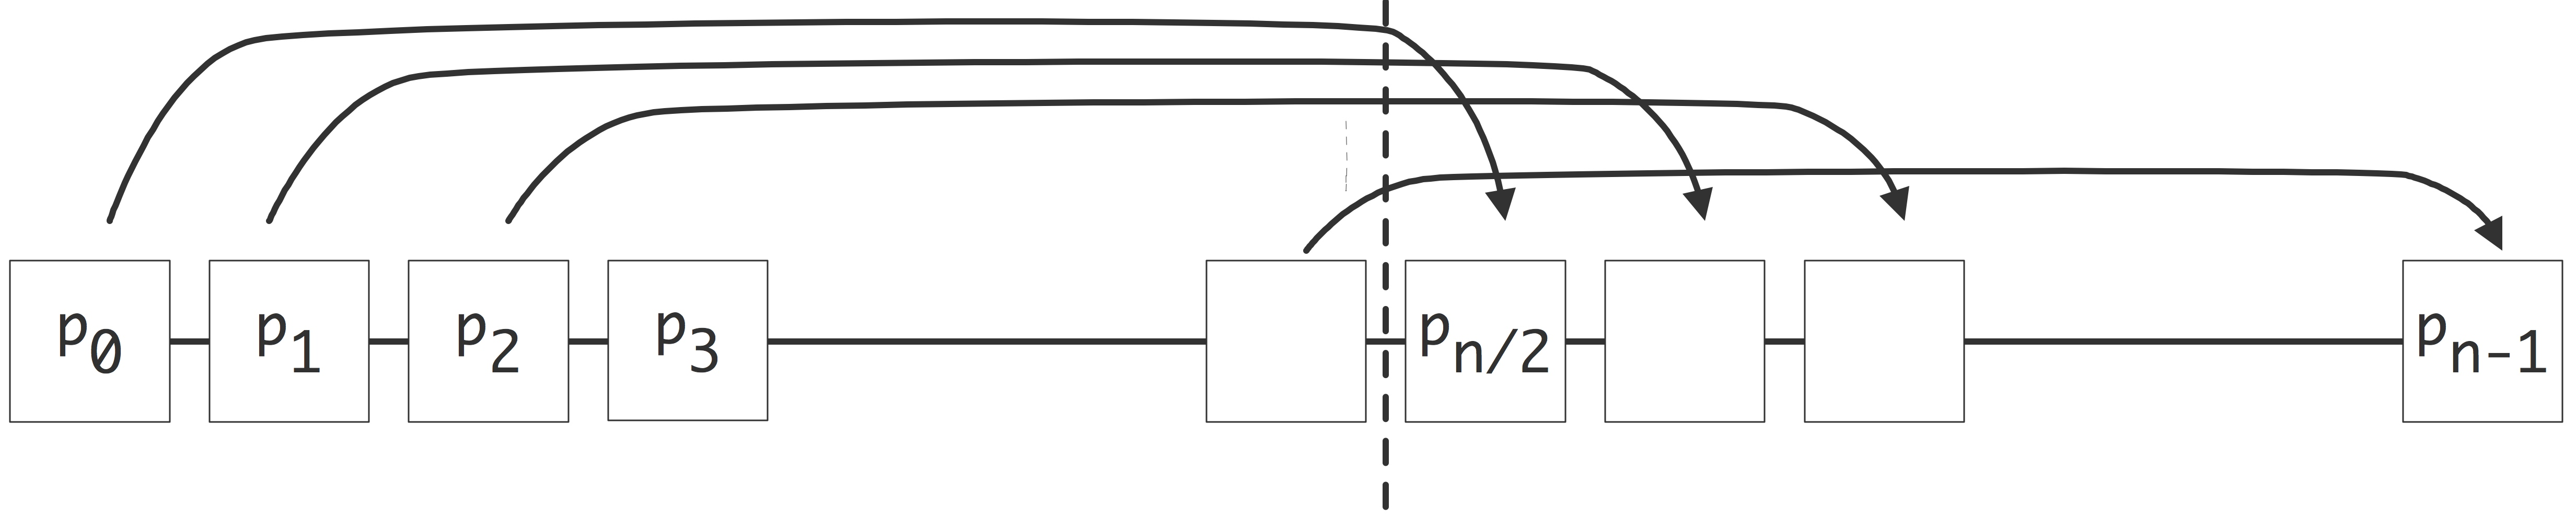
\includegraphics[scale=.09]{graphics/contention}
  \caption{Contention for a network link due to simultaneous messages}
  \label{fig:contention}
\end{figure}
This
sort of conflict is called \indexterm{congestion} or
\indexterm{contention}. Clearly, the more links a
parallel computer has, the smaller the chance of congestion.

A~precise way to describe the likelihood of congestion, is
to look at the \indexterm{bisection width}. This is defined as the
minimum number of links that have to be removed to partition the
processor graph into two unconnected graphs. For instance, consider
processors connected as a linear array, that is, processor $P_i$ is
connected to $P_{i-1}$ and~$P_{i+1}$. In this case the bisection width
is~1.

The bisection width~$w$ describes how many messages can, guaranteed,
be under way simultaneously in a parallel computer. Proof: take $w$
sending and $w$ receiving processors. The $w$ paths thus defined are
disjoint: if they were not, we could separate the processors into two
groups by removing only~$w-1$ links. 

In practice, of course, more than
$w$ messages can be under way simultaneously. For instance, in a
linear array, which has $w=1$, $P/2$~messages can be sent and received
simultaneously if all communication is between neighbours, and if a
processor can only send or receive, but not both, at any one time. If
processors can both send and receive simultaneously, $P$~messages can
be under way in the network.

Bisection width also describes \indexterm{redundancy} in a network: if
one or more connections are malfunctioning, can a message
still find its way from sender to receiver?

While bisection width is a measure expressing a number of wires, in
practice we care about the capacity through those wires. The relevant
concept here is \indexterm{bisection bandwidth}: the bandwidth across
the bisection width, which is the product of the bisection width, and
the capacity (in bits per second) of the wires.  
%
Bisection bandwidth
can be considered as a measure for the bandwidth that can be attained
if an arbitrary half of the processors communicates with the other
half.
Bisection bandwidth is a more realistic measure than the
\indextermsub{aggregate}{bandwidth} which is sometimes quoted
and which is defined
as the  total data rate if every processor is sending: the number of
processors times the bandwidth of a connection times the number of
simultaneous sends a processor can perform. This can be quite
a high number, and it is typically not representative of the
communication rate that is achieved in actual applications.

\Level 1 {Busses}

The first interconnect design we consider is to have all processors
on the same \indextermsub{memory}{bus}. This design connects
all processors directly to the same memory pool, so it offers
a \indexac{UMA} or \indexac{SMP} model.

The main disadvantage of using a bus is the limited scalability,
since only one processor at a time can do a memory access. To overcome this,
we need to assume that processors are slower than memory,
or that the processors have cache or other local memory to operate out of.
In the latter case, maintaining \indextermbus{cache}{coherence}
is easy with a bus by letting processors listen to all the memory traffic
on the bus~-- a~process known as \indexterm{snooping}.

\Level 1 {Linear arrays and rings}

A simple way to hook up multiple processors is to connect them in a
\emph{linear array}\index{linear array (of processors)}: every processor has a number~$i$, and
processor~$P_i$ is connected to $P_{i-1}$ and~$P_{i+1}$. The first and
last processor are possible exceptions: if they are connected to each
other, we call the architecture a \indexterm{ring network}.

This solution requires each processor to have two network connections,
so the design is fairly simple.

\begin{exercise}
  What is the bisection width of a linear array? Of a ring?
\end{exercise}

\begin{exercise}
  With the limited connections of a linear array, you may have to be
  clever about how to program parallel algorithms. For instance,
  consider a `broadcast' operation: processor~$0$ has a data item that
  needs to be sent to every other processor. 

  We make the following simplifying assumptions:
  \begin{itemize}
  \item a processor can send any number of messages simultaneously,
  \item but a wire can can carry only one message at a time; however,
    \item communication between any two processors takes unit time,
      regardless of the number of processors in between them.
  \end{itemize}

  In a fully connected network or a star network
  you can simply write
  \begin{tabbing}
    for \=$i=1\ldots N-1$:\\ \>send the message to processor~$i$
  \end{tabbing}
  With the assumption that a processor can send multiple messages,
  this means that the operation is done in one step.

  Now consider a linear array. Show that, even with this unlimited capacity for
  sending, the above algorithm runs into trouble because of congestion.

  Find a better way to organize the send operations. Hint: pretend
  that your processors are connected as a binary tree. Assume that
  there are $N=2^n-1$ processors.
  Show that the broadcast can be done in $\log N$ stages, and that
  processors only need to be able to send a single message simultaneously.
\end{exercise}
This exercise is an example of \indexterm{embedding} a
`logical' communication pattern in a physical one.

\Level 1 {2D and 3D arrays}

A popular design for parallel computers is to organize the processors
in a two-dimensional or three-dimensional \indexterm{Cartesian mesh}.
This means that every processor has a coordinate $(i,j)$ or $(i,j,k)$,
and it is connected to its neighbours in all coordinate directions.
The processor design is still fairly simple: the number of network
connections (the degree of the connectivity graph) is twice the number
of space dimensions (2~or~3) of the network.

It is a fairly natural idea to have 2D or 3D networks, since the world
around us is three-dimensional, and computers are often used to model
real-life phenomena. If we accept for now that the physical model
requires \indexterm{nearest neighbour} type communications (which we
will see is the case in section~\ref{sec:2dbvp}), then a mesh computer
is a natural candidate for running physics simulations.

\begin{exercise}
  What is the diameter of a 3D cube of $n\times n\times n$ processors? What is the
  bisection width? How does that change if you add wraparound torus
  connections?
\end{exercise}

\begin{exercise}
  Your parallel computer has its processors organized in a 2D grid.
  The chip manufacturer comes out with a new chip with same clock
  speed that is dual core instead of single core, and that will fit in
  the existing sockets. Critique the following argument: `the amount of
  work per second that can be done (that does not involve communication)
  doubles; since the network stays the same, the bisection bandwidth
  also stays the same, so I can reasonably expect my new machine to
  become twice as fast\footnote{With the numbers one and two replaced
    by higher numbers, this is actually not a bad description of
    current trends in processor design.}.'
\end{exercise}

Grid-based designs often have so-called \emph{wrap-around} or
\indexterm{torus} connections, which connect the left and right sides
of a 2D grid, as well as the top and bottom. This is illustrated in
figure~\ref{fig:torus}.
\begin{figure}[th]
  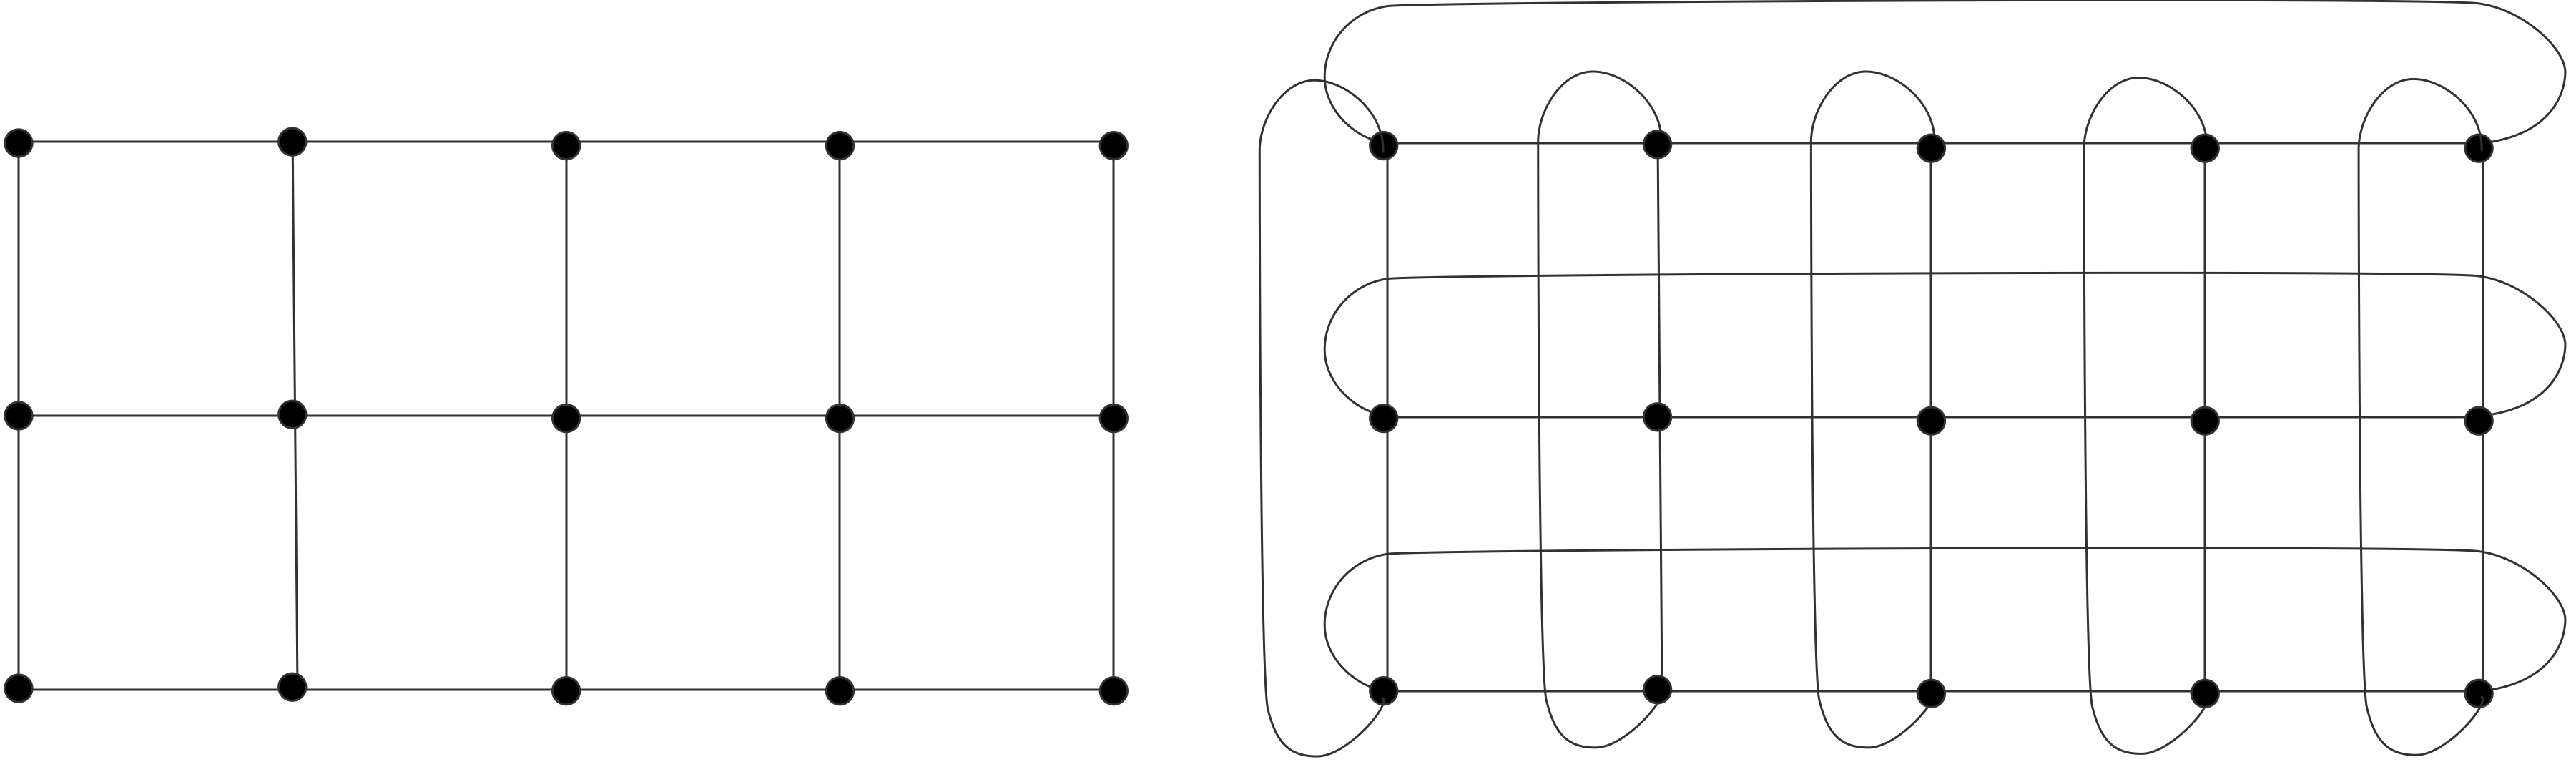
\includegraphics[scale=.11]{graphics/torus}
  \caption{A 2D grid with torus connections}
  \label{fig:torus}
\end{figure}

Some computer designs claim to be a grid of high dimensionality, for
instance~5D, but not all dimensionals are equal here. For instance, a 3D
grid where each \indexterm{node} is a quad-socket 
quad-core can be considered as a
5D grid. However, the last two dimensions are fully connected.

\Level 1 {Hypercubes}
\label{sec:hypercube}

Above we gave a hand-waving argument for the suitability of
mesh-organized processors based on the prevalence of nearest
neighbour communications. However, sometimes sends and receives
between arbitrary processors occur. One example of this is the
above-mentioned broadcast. For this reason, it is desirable to have a
network with a smaller diameter than a mesh. On the other hand we want
to avoid the complicated design of a fully connected network.

\begin{wrapfigure}{r}{3in}
  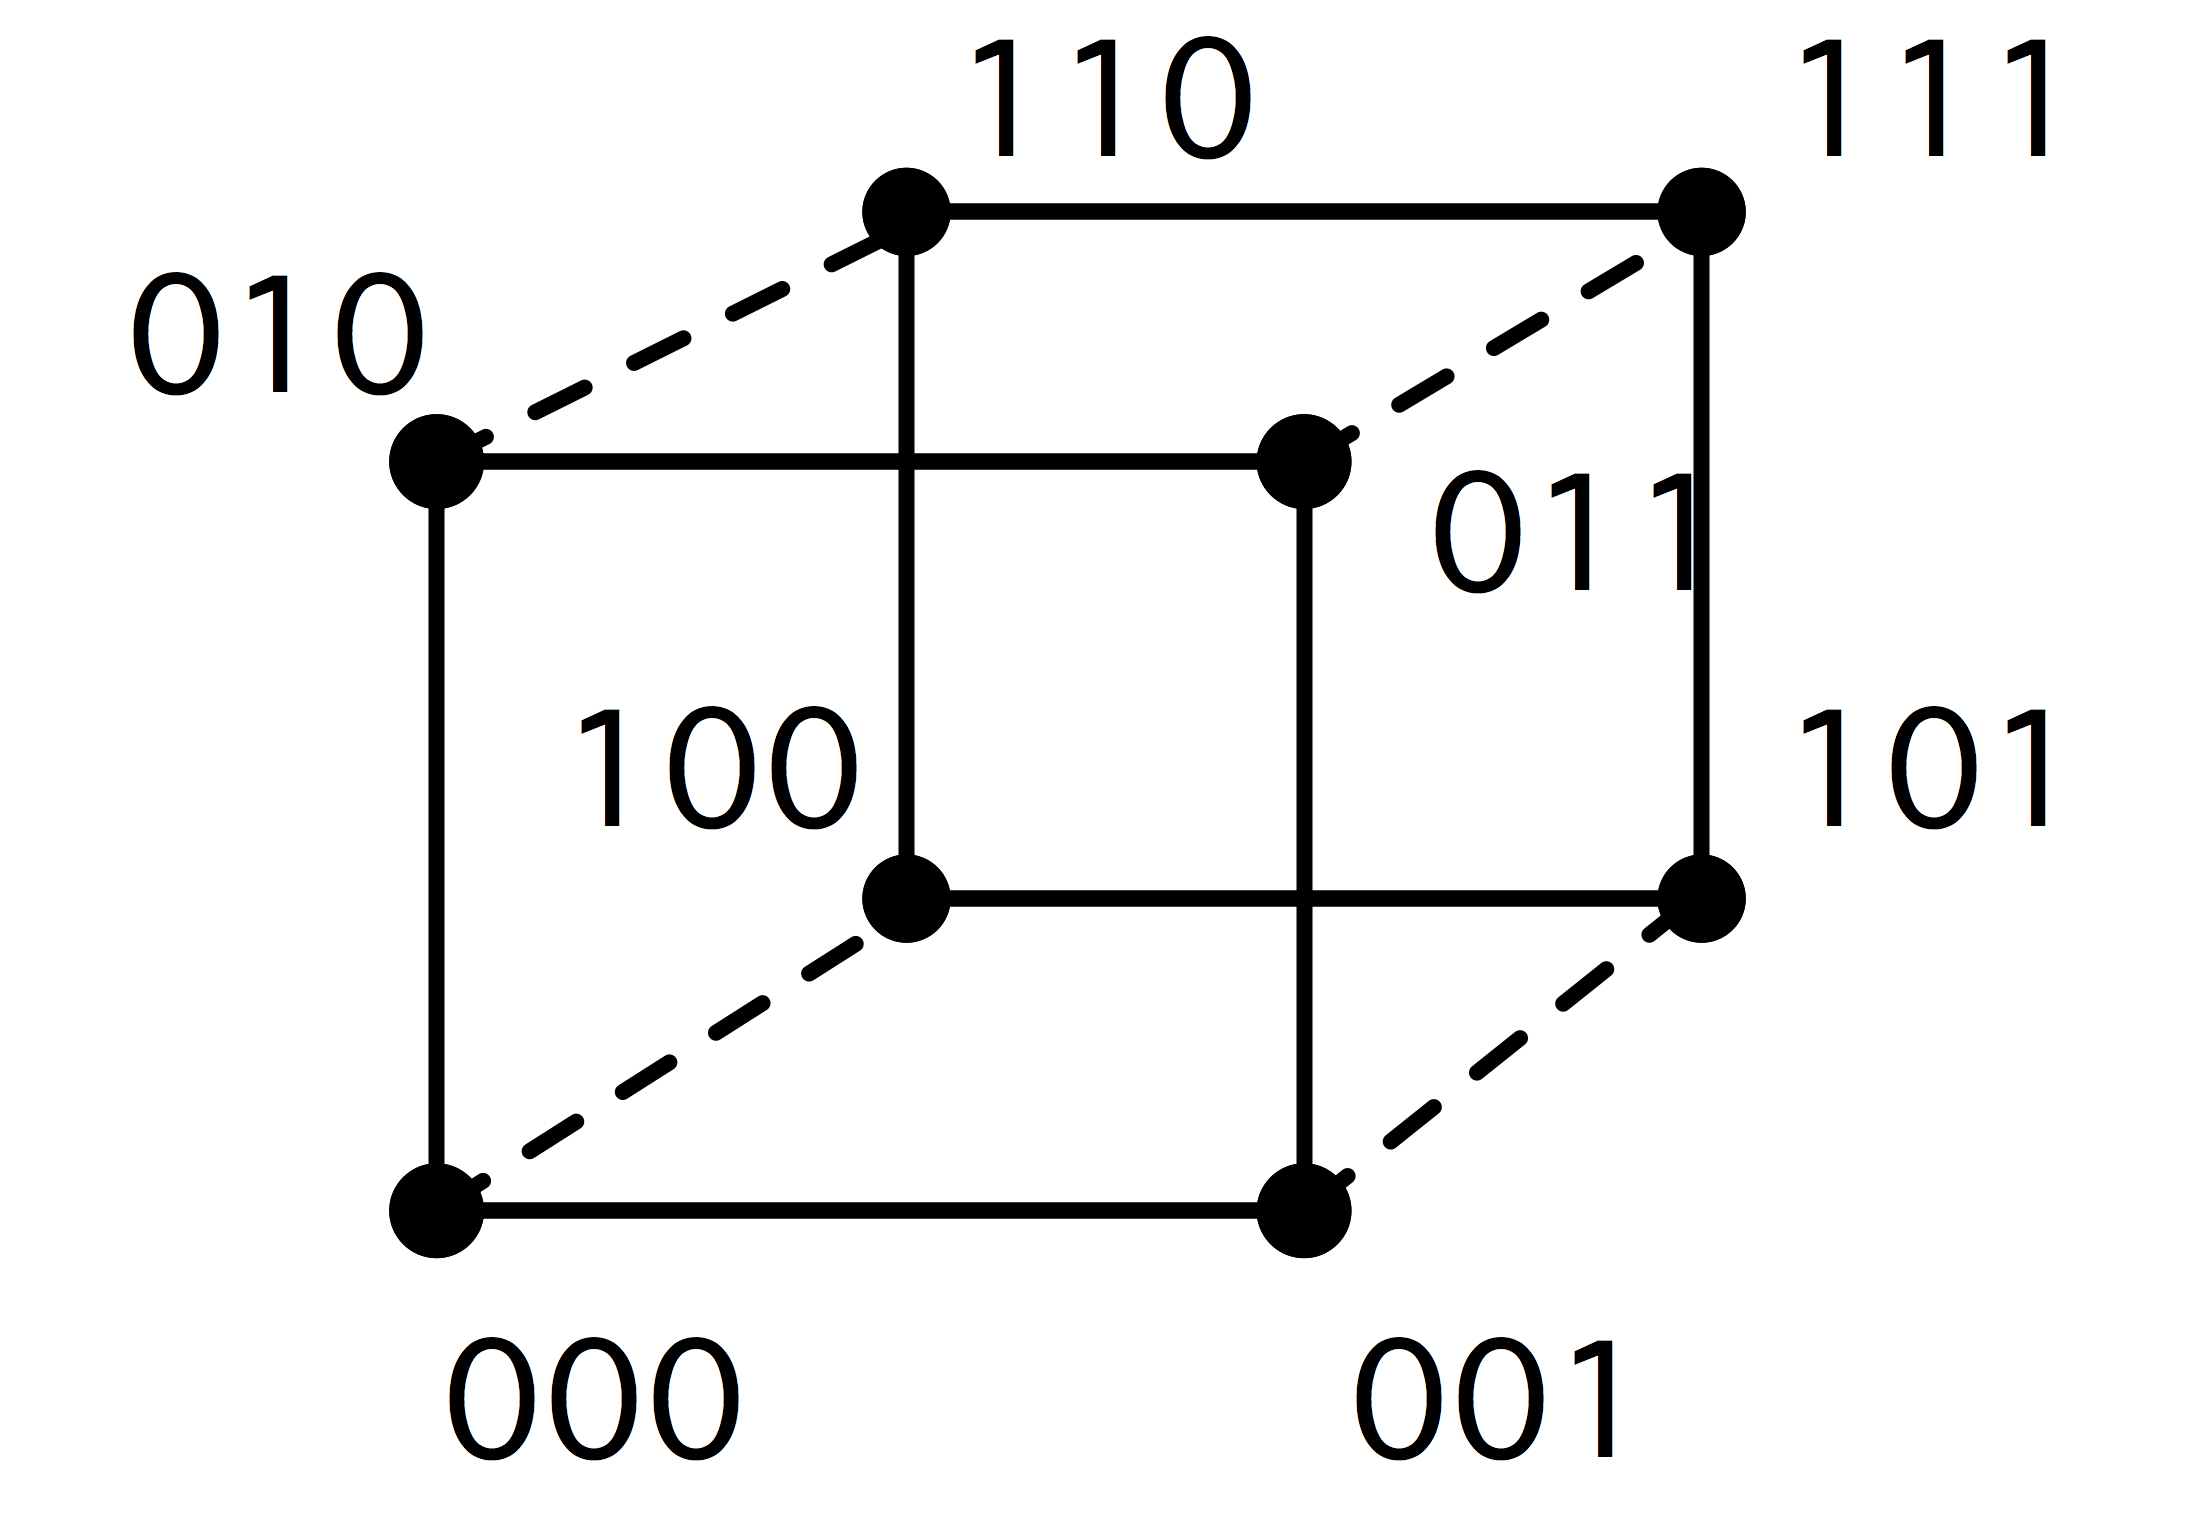
\includegraphics[scale=.081]{graphics/hypercubenumber}
  \caption{Numbering of the nodes of a hypercube}
  \label{fig:cubenumber}
\end{wrapfigure}
%
A good intermediate solution is the \indexterm{hypercube} design. An
$n$-dimensional hypercube computer has $2^n$ processors, with each
processor connected to one other in each dimension; see
figure~\ref{fig:hypercube}. 

\begin{figure}[t]
  \begin{quote}
  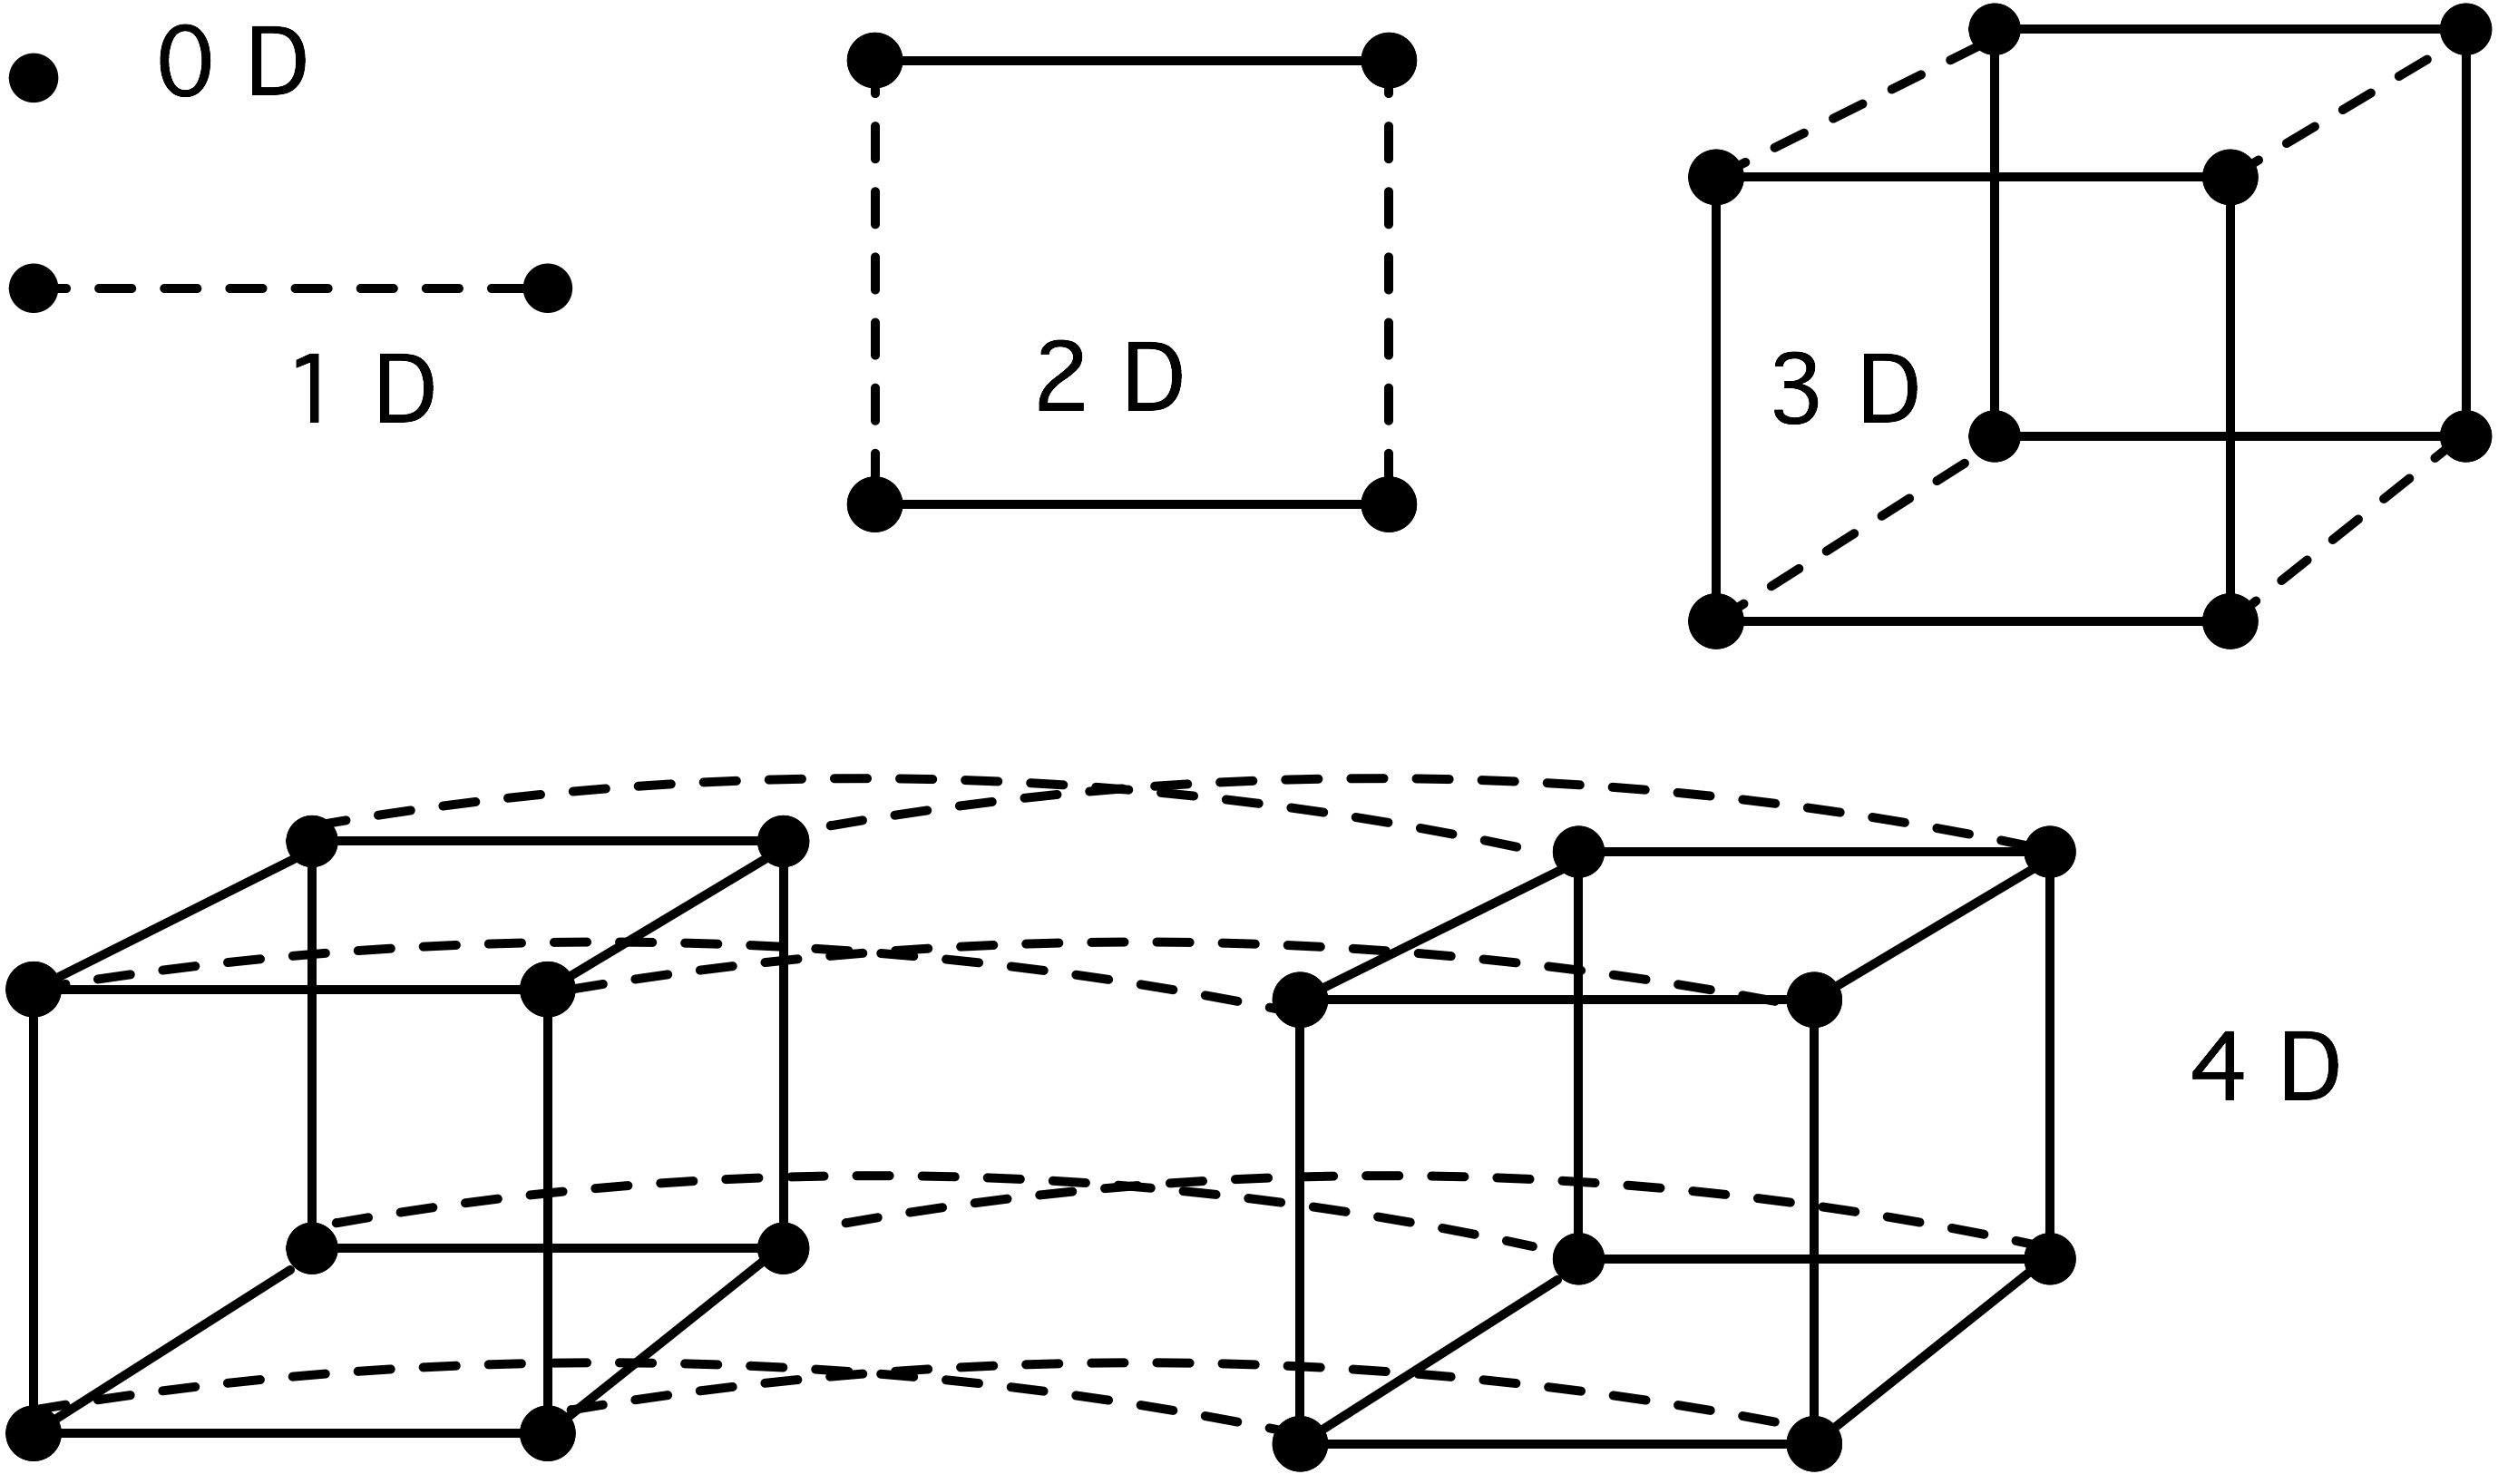
\includegraphics[scale=.12]{graphics/hypercubes}
  \end{quote}
  \caption{Hypercubes}
  \label{fig:hypercube}
\end{figure}

%% \begin{figure}[ht]
%%   \centering
%%   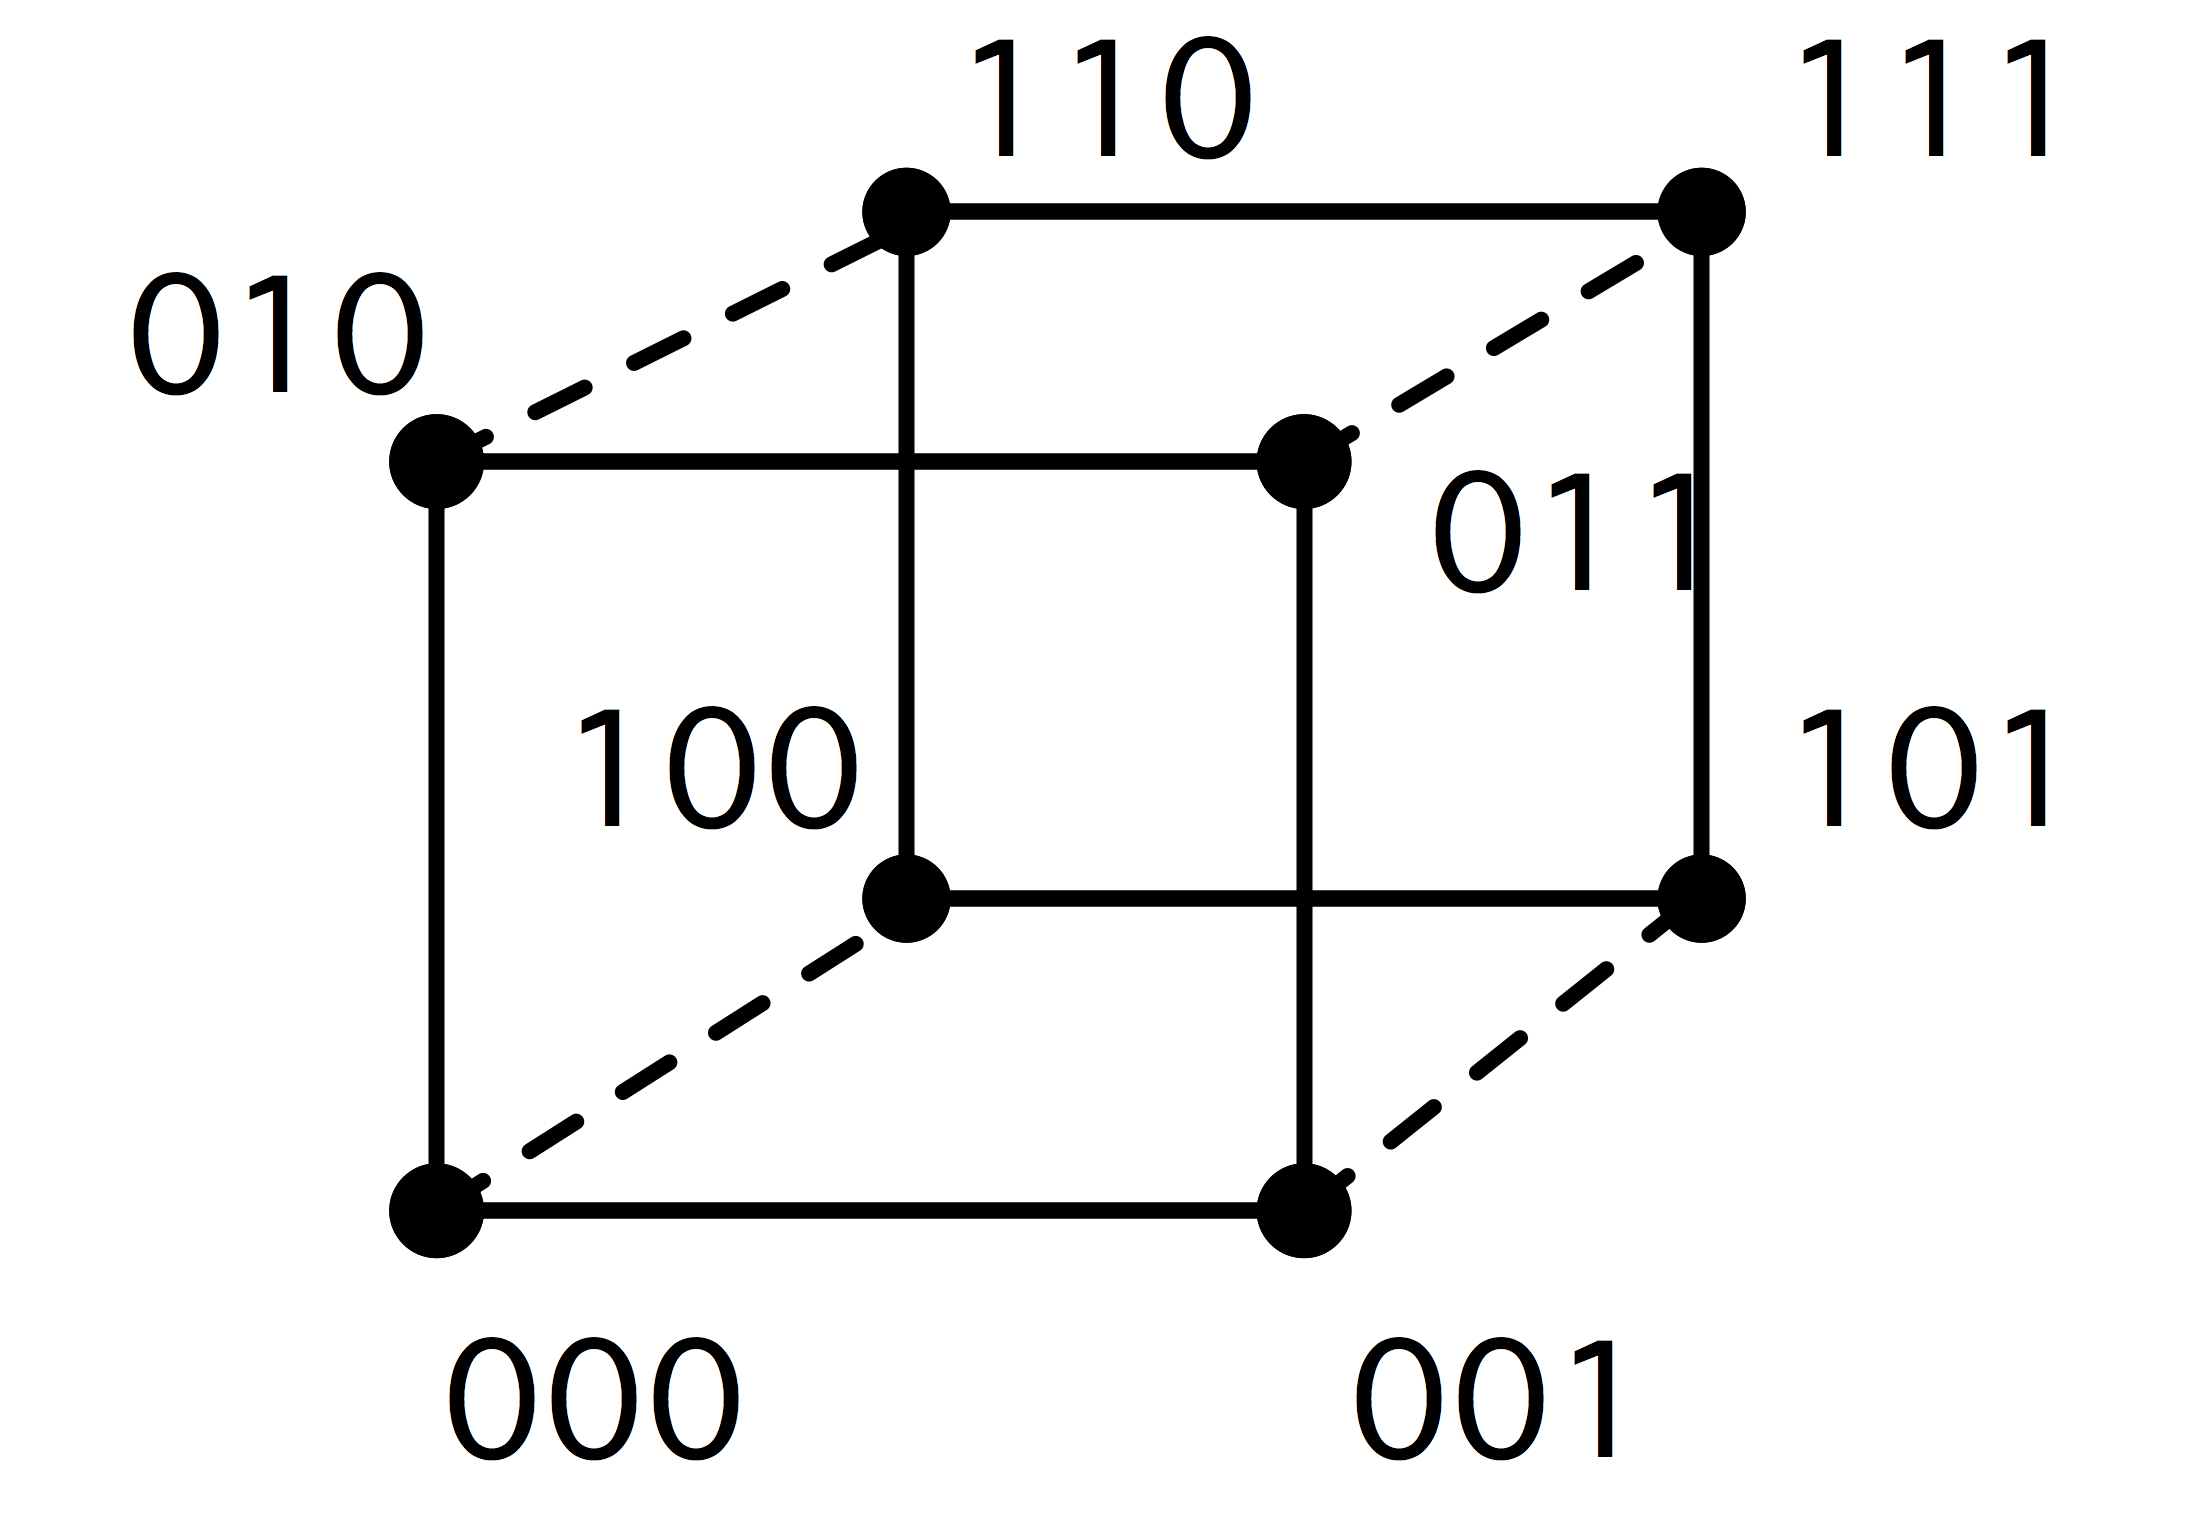
\includegraphics[scale=.1]{graphics/hypercubenumber}
%%   \caption{Numbering of the nodes of a hypercube}
%%   \label{fig:cubenumber}
%% \end{figure}

An easy way to describe this is to give each processor an address
consisting of $d$~bits: we give each node of a hypercube a number that
is the bit pattern describing its location in the cube; see
figure~\ref{fig:cubenumber}.

With this numbering scheme, a~processor is then connected to all others
that have an address that differs by exactly one bit. This means that,
unlike in a grid, a processor's neighbours do not have numbers
that differ by~1 or~$\sqrt P$, but by~$1,2,4,8,\ldots$.

The big advantages of a hypercube design are the small diameter and
large capacity for traffic through the network.
\begin{exercise}
  What is the diameter of a hypercube? What is the bisection width?
\end{exercise}

One disadvantage is the fact that the processor design is dependent on
the total machine size. In practice, processors will be designed with
a maximum number of possible connections, and someone buying a smaller
machine then will be paying for unused capacity.  Another
disadvantage is the fact that extending a given machine can only be
done by doubling it: other sizes than $2^p$ are not possible.

\begin{exercise}
  Consider the parallel summing example of
  section~\ref{sec:parallel-intro}, and give the execution time of a
  parallel implementation on a
  hypercube. Show that 
  the theoretical speedup from the example is attained (up to a
  factor) for the implementation on a hypercube.
\end{exercise}

\Level 2 {Embedding grids in a hypercube}

\def\graycodepicture{
\begin{wrapfigure}{r}{3in}
  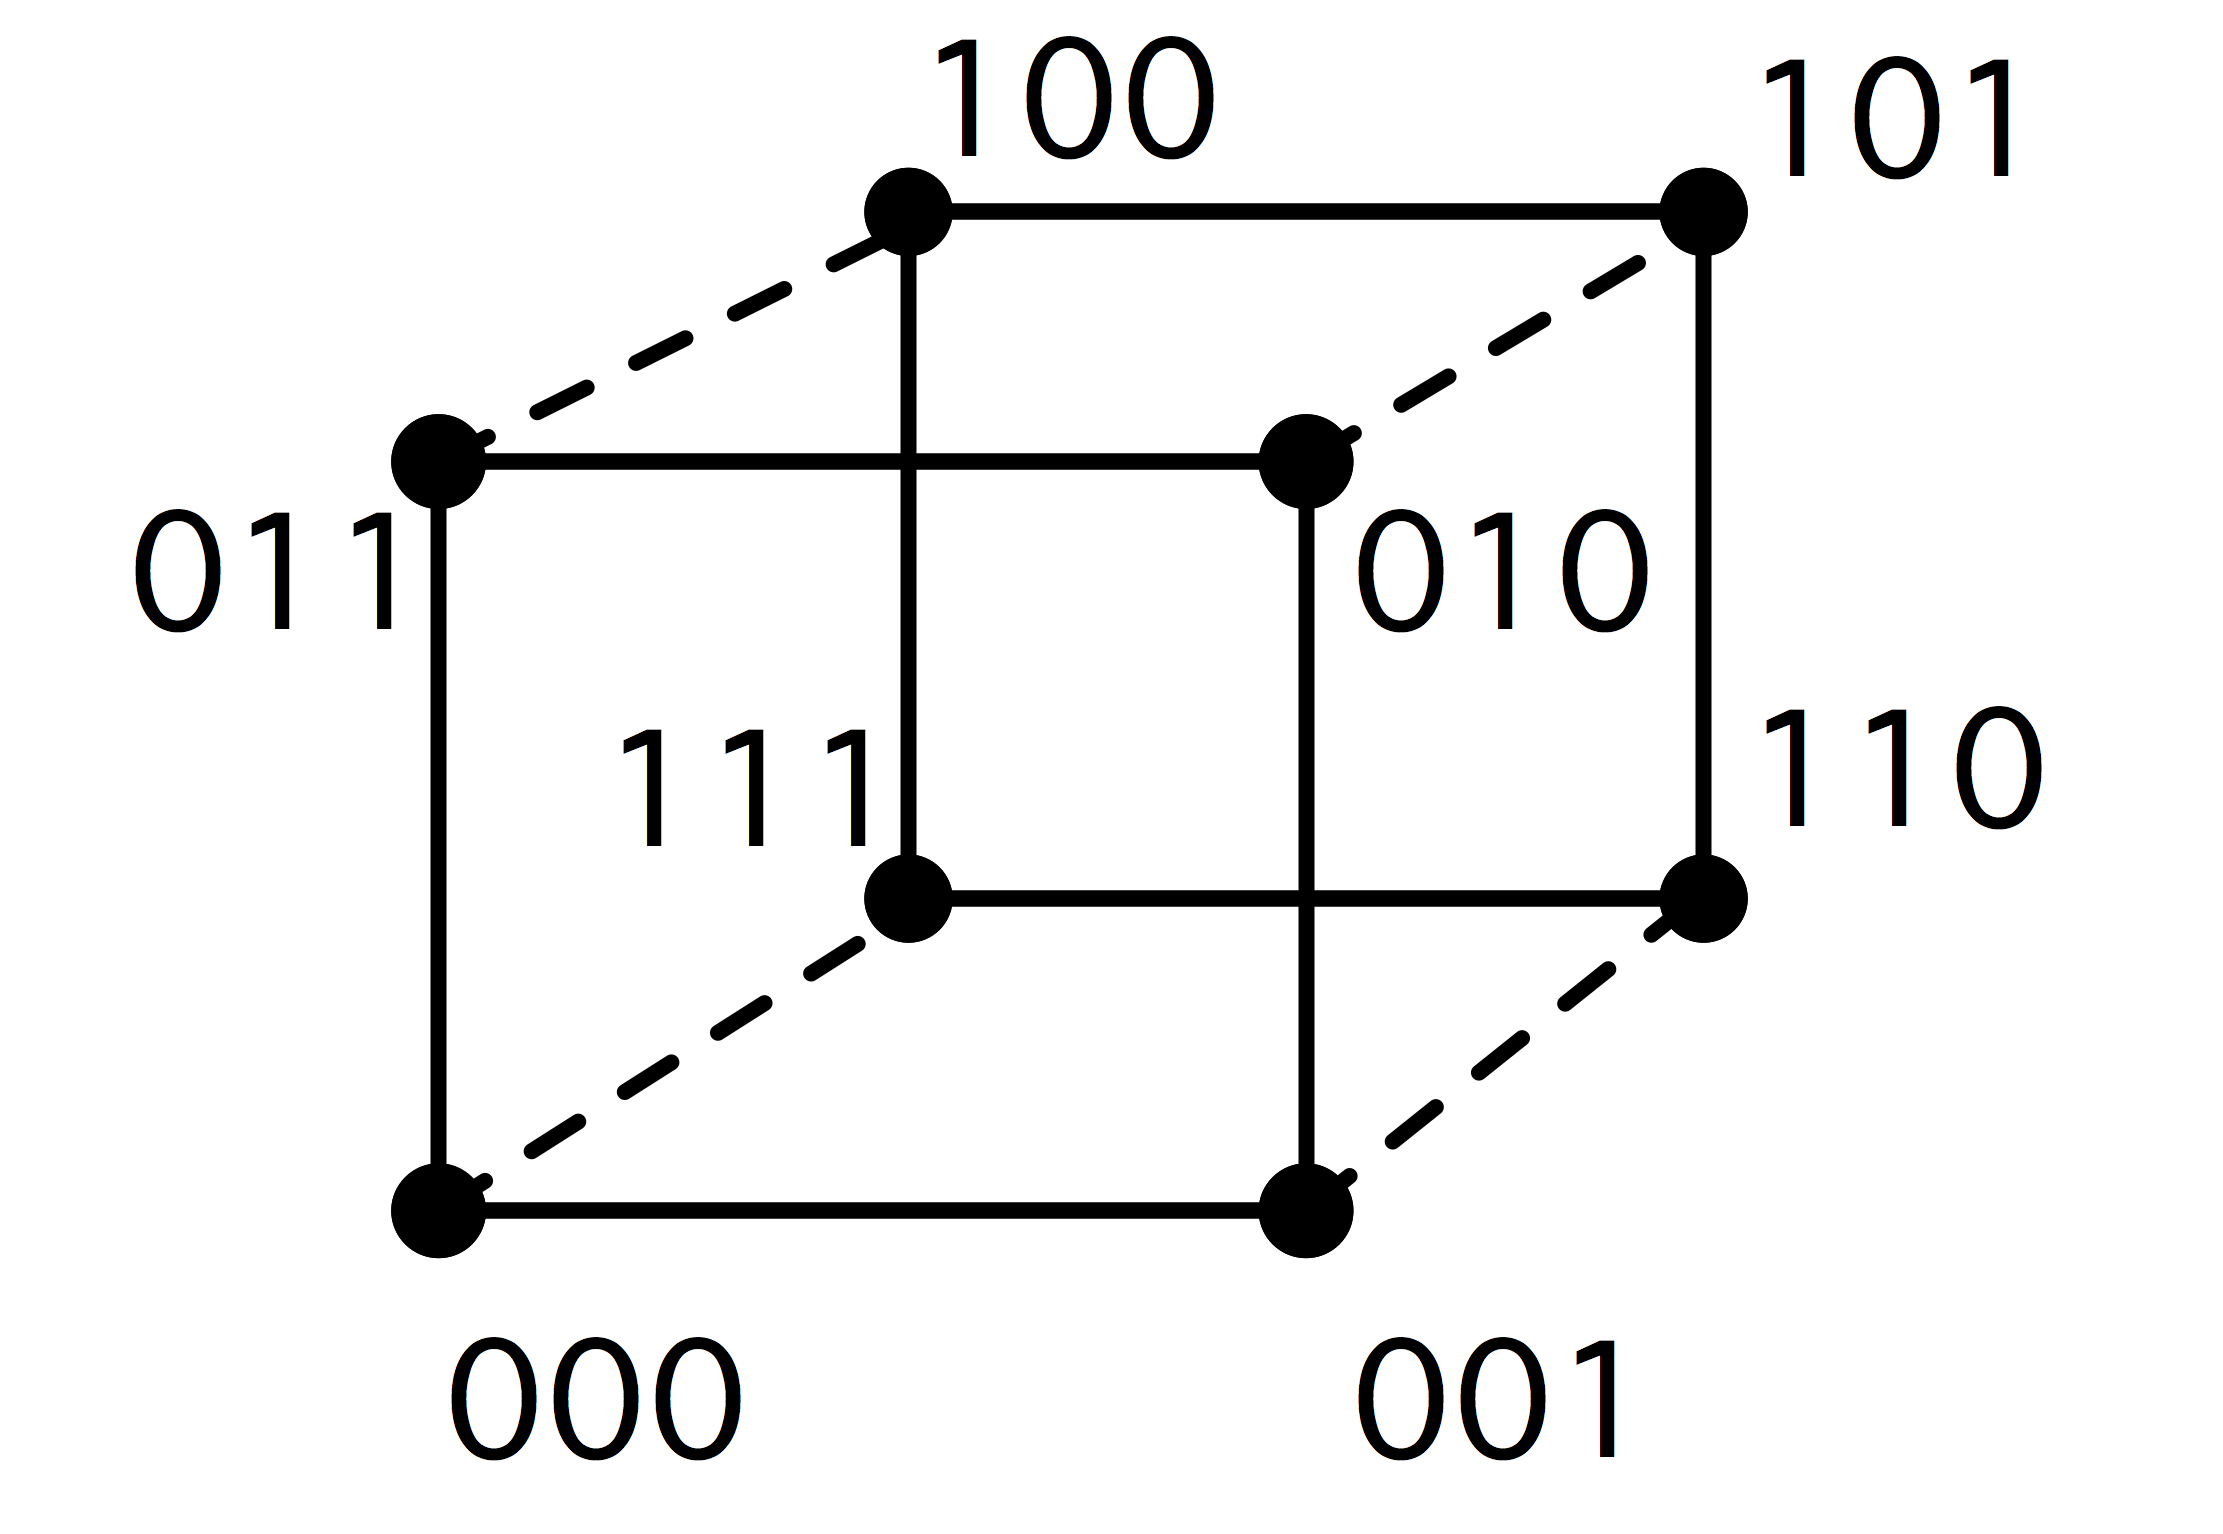
\includegraphics[scale=.081]{graphics/hypercubegraynumber}
  \caption{Gray code numbering of the nodes of a hypercube}
  \label{fig:cubegraynumber}
\end{wrapfigure}
}

Above we made the argument that mesh-connected processors are a
logical choice for many applications that model physical phenomena.
Hypercubes do not look like a mesh, but they have enough
connections that they can simply pretend to be a mesh by ignoring
certain connections. 

\begin{lulu}
\graycodepicture  
\end{lulu}
%
Let's say that we want the structure of a 1D array: we want processors
with a numbering so that processor $i$ can directly send data to $i-1$
and~$i+1$. We can not use the obvious numbering of
nodes as in figure~\ref{fig:cubenumber}. For instance, node~1 is
directly connected to node~0, but has a distance of~2 to node~2. The
right neighbour of node~3 in a ring, node~4, even has the maximum
distance of~3 in this hypercube. Clearly we need to renumber the nodes
in some way.

What we will show is that
it's possible to walk through a hypercube, touching
every corner exactly once, which is equivalent to embedding a 1D mesh
in the hypercube.

\begin{figure}[ht]
\hbox{\fbox{1D Gray code}:
$\vcenter{$
\begin{array}{rll}
  \hphantom{1D code and reflection:}&0&1\\
\end{array}$}
$}

\hbox{\fbox{2D Gray code}:
$\vcenter{$
\begin{array}{rccccc}
  \hbox{1D code and reflection:}&0&1&\vdots&1&0\\
  \hbox{append 0 and 1 bit:}&0&0&\vdots&1&1
\end{array}$}
$}

\hbox{\fbox{3D Gray code}:
$\vcenter{$
\begin{array}{rccccccccc}
  \hbox{2D code and reflection:}&0&1&1&0&\vdots&0&1&1&0\\
  &0&0&1&1&\vdots&1&1&0&0\\
  \hbox{append 0 and 1 bit:}&0&0&0&0&\vdots&1&1&1&1
\end{array}$}
$}

  \caption{Gray codes}
  \label{fig:graycode}
\end{figure}

\begin{notlulu}
  \graycodepicture
\end{notlulu}
%
The basic concept here is a (binary reflected) \indexterm{Gray
  code}~\cite{Gray:graycodepatent}. This is a way of ordering the
binary numbers $0\ldots2^d-\nobreak1$ as $g_0,\ldots g_{2^d-1}$ so that $g_i$
and $g_{i+1}$ differ in only one bit. Clearly, the ordinary binary
numbers do not satisfy this: the binary representations for 1~and~2
already differ in two bits. Why do Gray codes help us? Well, since
$g_i$ and $g_{i+1}$ differ only in one bit, it means they are the
numbers of nodes in the hypercube that are directly connected.

Figure~\ref{fig:graycode} illustrates how to construct a Gray
code. The procedure is recursive, and can be described informally as
`divide the cube into two subcubes, number the one subcube, cross over
to the other subcube, and number its nodes in the reverse order of the
first one'. The result for a 2D cube is in figure~\ref{fig:cubegraynumber}.

Since a Gray code offers us a way to embed a one-dimensional `mesh'
into a hypercube, we can now work our way up.
\begin{exercise}
  Show how a square mesh of $2^{2d}$ nodes can be embedded in a
  hypercube by appending the bit patterns of the embeddings of two
  $2^d$ node cubes. How would you accommodate a mesh of $2^{d_1+d_2}$
  nodes? A three-dimensional mesh of $2^{d_1+d_2+d_3}$ nodes?
\end{exercise}

\Level 1 {Switched networks}
\label{sec:crossbar}

\def\crossbarfig{
\begin{wrapfigure}{r}{2.5in}%[ht]
%  \begin{quote}
  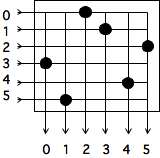
\includegraphics[scale=.7]{graphics/crossbar}
%  \end{quote}
  \caption{A simple cross bar connecting 6 inputs to 6 outputs}
  \label{fig:crossbar}
\end{wrapfigure}
}

Above, we briefly discussed fully connected processors. They are
impractical if the connection is made by making a large number of
wires between all the processors. There is another possibility,
however, by connecting all the processors to a \indexterm{switch} or
switching network. Some popular network designs are the
\indexterm{crossbar}, the \indexterm{butterfly exchange}, and the
\indexterm{fat tree}.

Switching networks are made out of switching elements, each of which
have a small number (up to about a dozen) of inbound and outbound
links. By hooking all processors up to some switching element, and
having multiple stages of switching, it then becomes possible to
connect any two processors by a path through the network.

\Level 2 {Cross bar}

\begin{notlulu}
  \crossbarfig
\end{notlulu}
%
\begin{lulu}
  \crossbarfig
\end{lulu}
%
The simplest switching network is a cross bar, an arrangement of $n$
horizontal and vertical lines, with a switch element on each
intersection that determines whether the lines are connected; see
figure~\ref{fig:crossbar}. If we designate the horizontal lines as
inputs the vertical as outputs, this is clearly a way of having $n$
inputs be mapped to $n$ outputs. Every combination of inputs and
outputs (sometimes called a `permutation') is allowed.

One advantage of this type of network is that no connection 
blocks another.
The main disadvantage  is that the number of 
switching elements is~$n^2$, a~fast growing function of the
number of processors~$n$.

\Level 2 {Butterfly exchange}
\index{Omega network|see{butterfly exchange}}
\index{butterfly exchange|(textbf}

\begin{figure}[ht]
  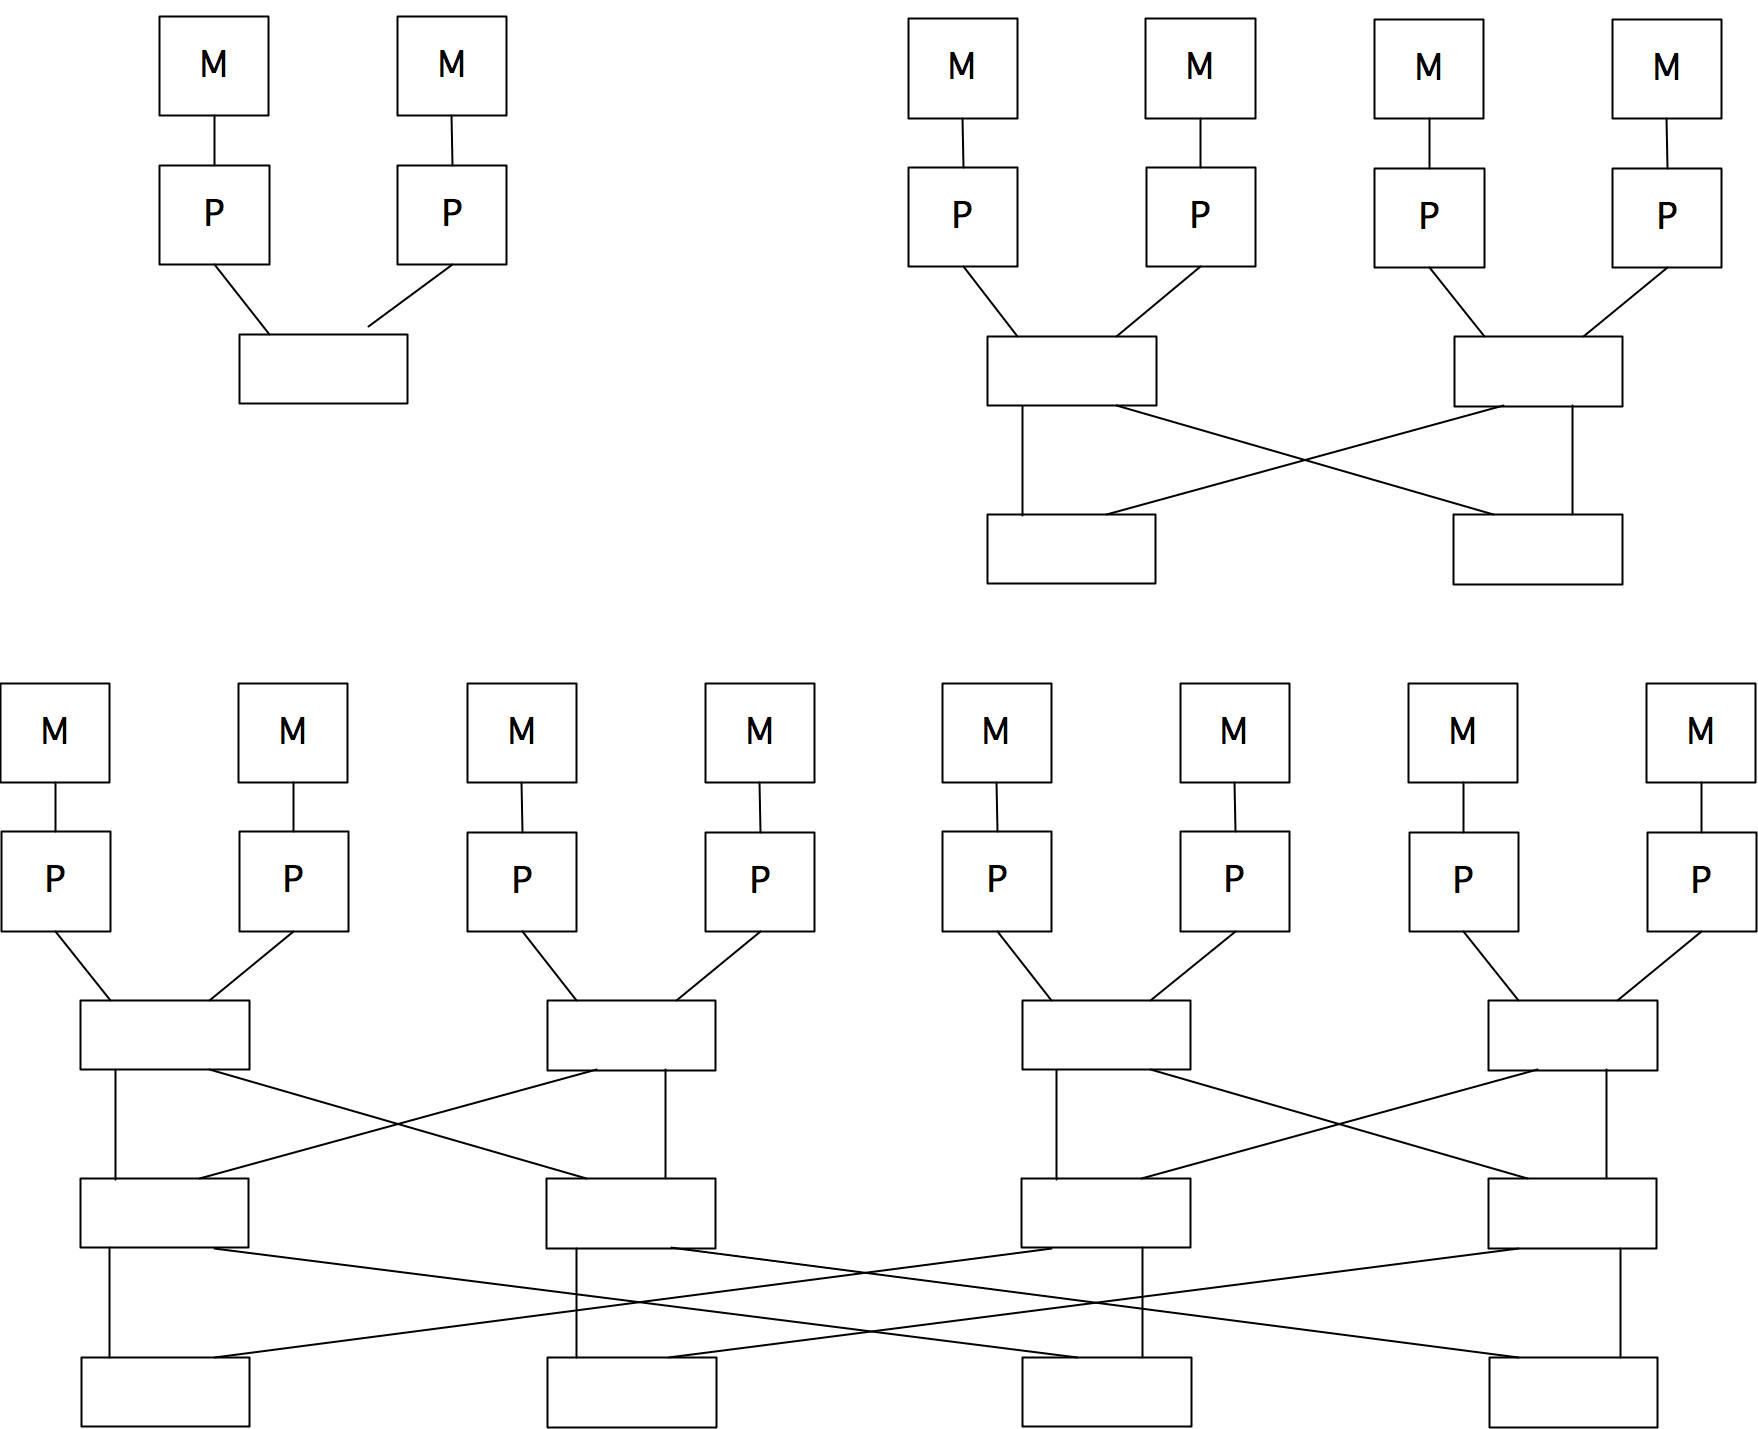
\includegraphics[scale=.06]{butterflys}
  \caption{Butterfly exchange networks for 2,4,8 processors, each with
    a local memory}
  \label{fig:butterfly}
\end{figure}

\emph{Butterfly exchange} networks are built out of small switching
elements, and they have multiple stages: as the number of processors
grows, the number of stages grows with it. Figure~\ref{fig:butterfly}
shows shows butterfly networks to connect 2,4,~and~8 processors, each
with a local memory. (Alternatively, you could put all processors at
one side of the network, and all memories at the other.)

As you can see in figure~\ref{fig:butterflyroute}, butterfly exchanges
allow several processors to access memory simultaneously. Also, their
access times are identical, so exchange networks are a way of
implementing a \indexac{UMA} architecture; see
section~\ref{sec:uma}. One computer that was based on a Butterfly
exchange network was the \indextermbus{BBN}{Butterfly}\footnote
{\url{http://en.wikipedia.org/wiki/BBN_Butterfly}}.
In section~\ref{sec:stampede-fattree} we will see how these ideas are
realized in a practical cluster.

\begin{figure}[ht]
  \begin{quote}
  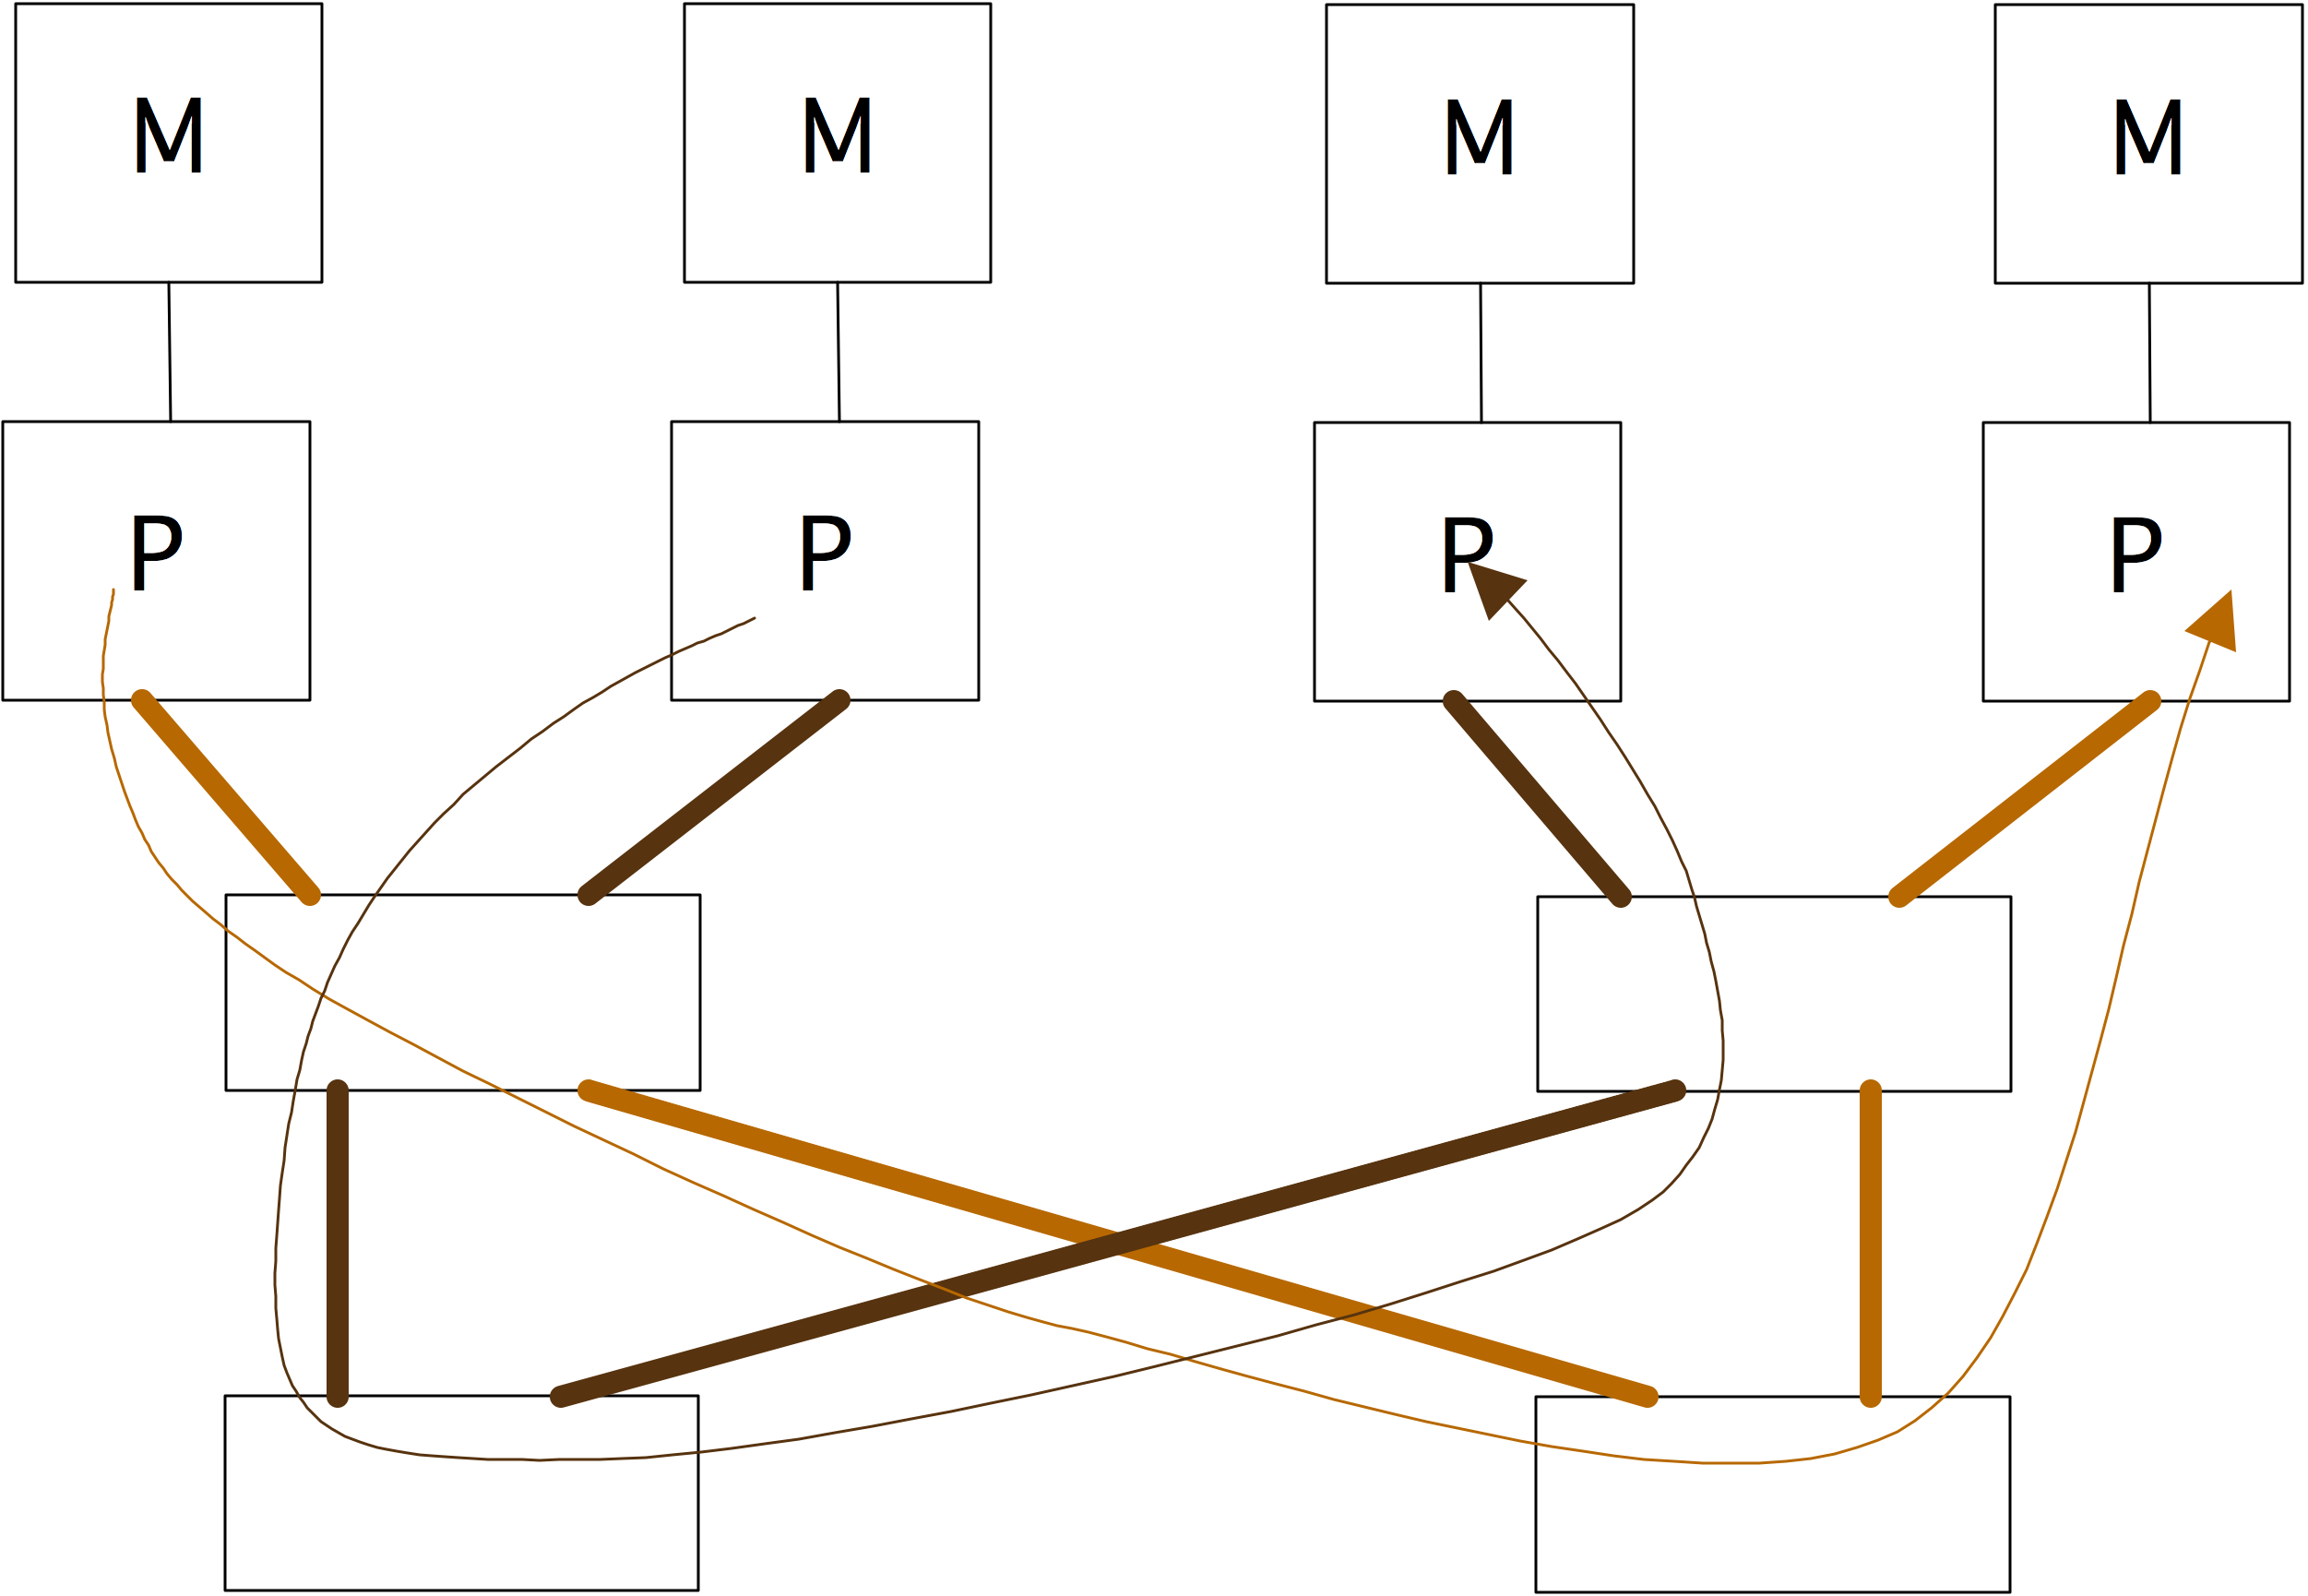
\includegraphics[scale=.1]{graphics/butterfly3}
  \end{quote}
  \caption{Two independent routes through a butterfly exchange network}
  \label{fig:butterflyroute}
\end{figure}

\begin{exercise}
For both the simple cross bar and the butterfly
exchange, the network needs to be expanded as the number of processors grows. 
Give the number of wires (of some unit length) and the number of switching
elements that is needed in both cases to connect~$n$ processors and memories. 
What is the time that a data packet needs to go from memory to processor,
expressed in the unit time that it takes to traverse a unit length of wire
and the time to traverse a switching element?
\end{exercise}

\emph{Packet routing}\index{routing!packet} through a butterfly
network is done based on considering the bits in the destination
address. On the $i$-th level the $i$-th digit is considered;
\begin{figure}[ht]
  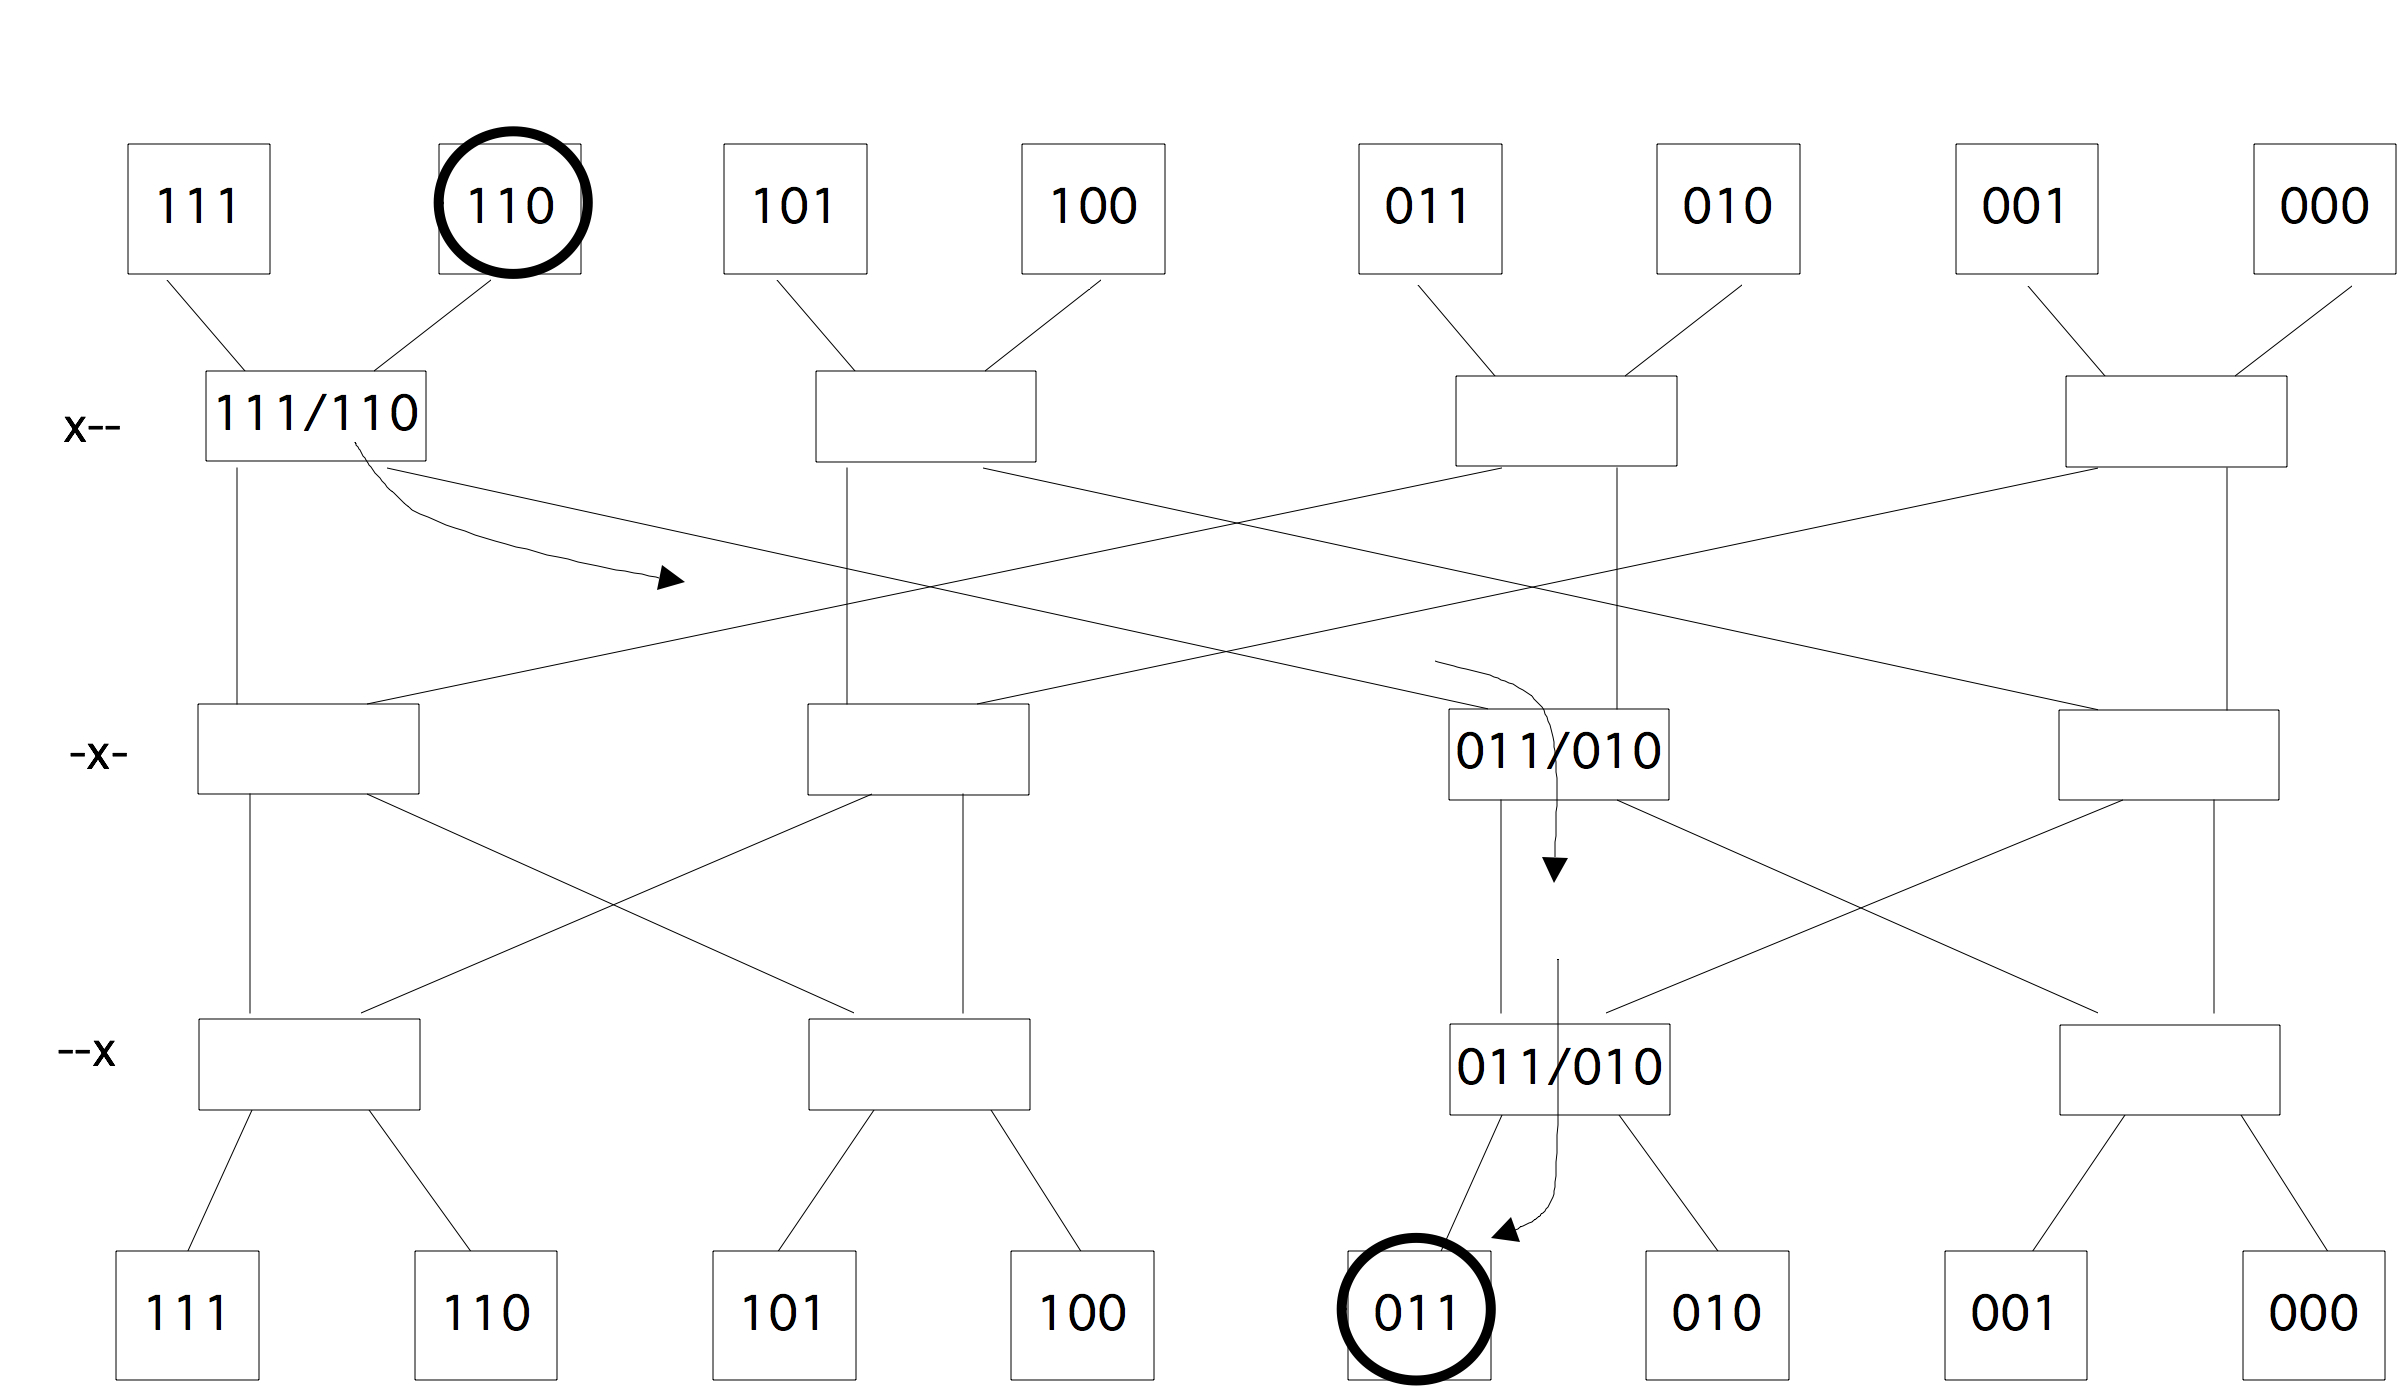
\includegraphics[scale=.18]{graphics/butterfly-route}
  \caption{Routing through a three-stage butterfly exchange network}
  \label{fig:butterfly-route}
\end{figure}
if this is~$1$, the left exit of the switch is taken, if~$0$, the
right exit. This is illustrated in
figure~\ref{fig:butterfly-route}. If we attach the memories to the
processors, as in figure~\ref{fig:butterflyroute}, we need only two
bits (to the last switch) but a further
three bits to describe the reverse route.

\index{butterfly exchange|)}

\Level 2 {Fat-trees}
\label{sec:fat-tree}
\index{fat tree|(}

If we were to connect switching nodes like a tree, there would be a
big problem with congestion close to the root since there are only two
wires attached to the root note.  Say we have a $k$-level tree, so
there are $2^k$ leaf nodes.  If all leaf nodes in the left subtree try
to communicate with nodes in the right subtree, we have $2^{k-1}$
messages going through just one wire into the root, and similarly out
through one wire.  A fat-tree is a tree network where each level has
the same total bandwidth, so that this congestion problem does not
occur: the root will actually have $2^{k-1}$ incoming and outgoing
wires attached~\cite{Greenberg89randomizedrouting}.
Figure~\ref{fig:fattree} shows this structure on the left;
\begin{figure}
  %\begin{quote}
\hbox{%
  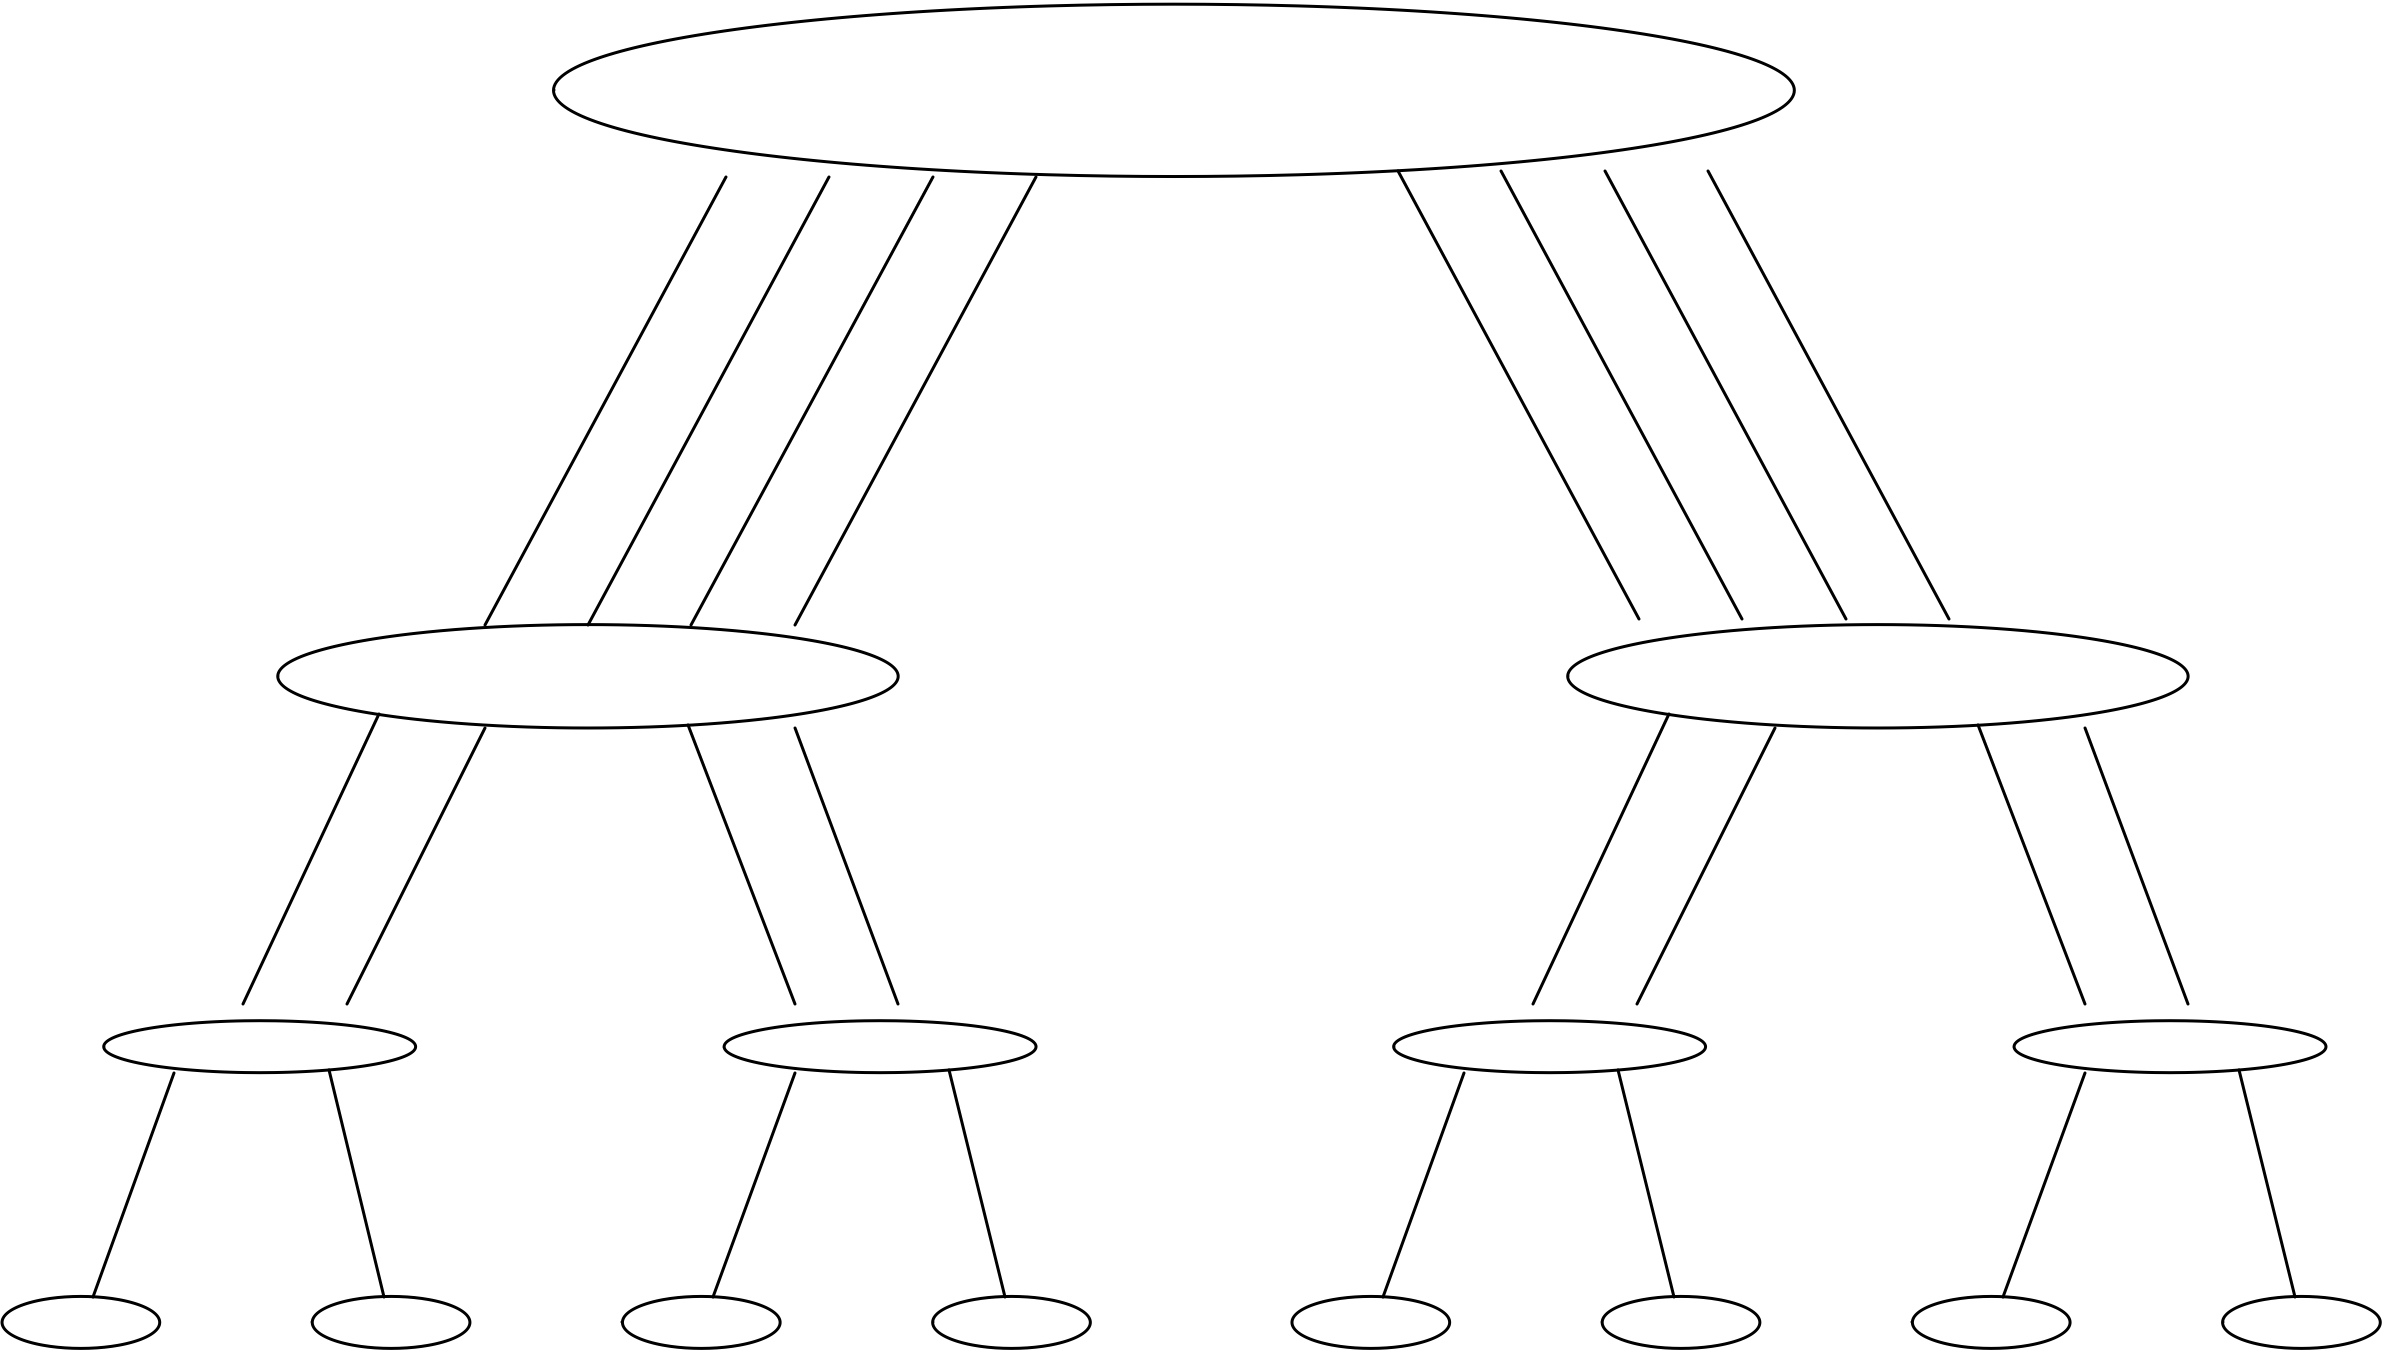
\includegraphics[scale=.12]{graphics/fattree5}
  \kern20pt
  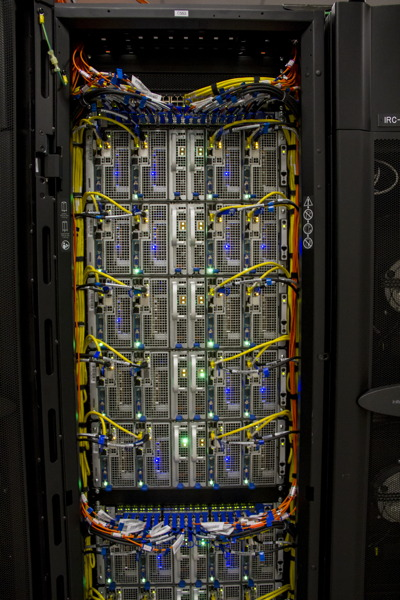
\includegraphics{stampede_leaf}
}
  %\end{quote}
  \caption{A fat tree with a three-level interconnect (left);
  the leaf switches in a cabinet of the Stampede cluster (right)}
  \label{fig:fattree}
\end{figure}
on the right is shown a cabinet of the \index{TACC}{Stampede cluster},
with a \indextermsub{leaf}{switch} for top and bottom half of the cabinet.

The first successful computer
architecture based on a fat-tree was the Connection Machines CM5.

In fat-trees, as in other switching networks, each message carries its
own routing information. Since in a fat-tree the choices are limited
to going up a level, or switching to the other subtree at the
current level, a message needs to carry only as many bits routing
information as there are levels, which is $\log_2n$ for $n$
processors.

\begin{exercise}
Show that the \indextermsub{bisection width of a}{fat tree} is $P/2$
where $P$ is the number of processor leaf nodes. Hint: show that there
is only one way of splitting a fat tree-connected set of processors
into two connected subsets.
\end{exercise}

The theoretical exposition of fat-trees in~\cite{Leiserson:fattree}
shows that fat-trees are optimal in some sense: it can deliver
messages as fast (up to logarithmic factors) as any other network that
takes the same amount of space to build. The underlying assumption of
this statement is that switches closer to the root have to connect
more wires, therefore take more components, and correspondingly are
larger. 
%
This argument, while theoretically interesting, is of no practical
significance, as the physical size of the network hardly plays a role
in the biggest currently available computers that use fat-tree
interconnect. For instance, in the Ranger supercomputer of The
University of Texas at Austin, the fat-tree switch connects 60,000
cores, yet takes less than 10 percent of the floor space.

A fat tree, as sketched above, would be costly to build, since for
every next level a new, bigger, switch would have to be designed. In
practice, therefore, a network with the characteristics of a fat-tree
is constructed from simple switching elements; see
figure~\ref{fig:fattreeclos}.
\begin{figure}[ht]
  \begin{quote}
    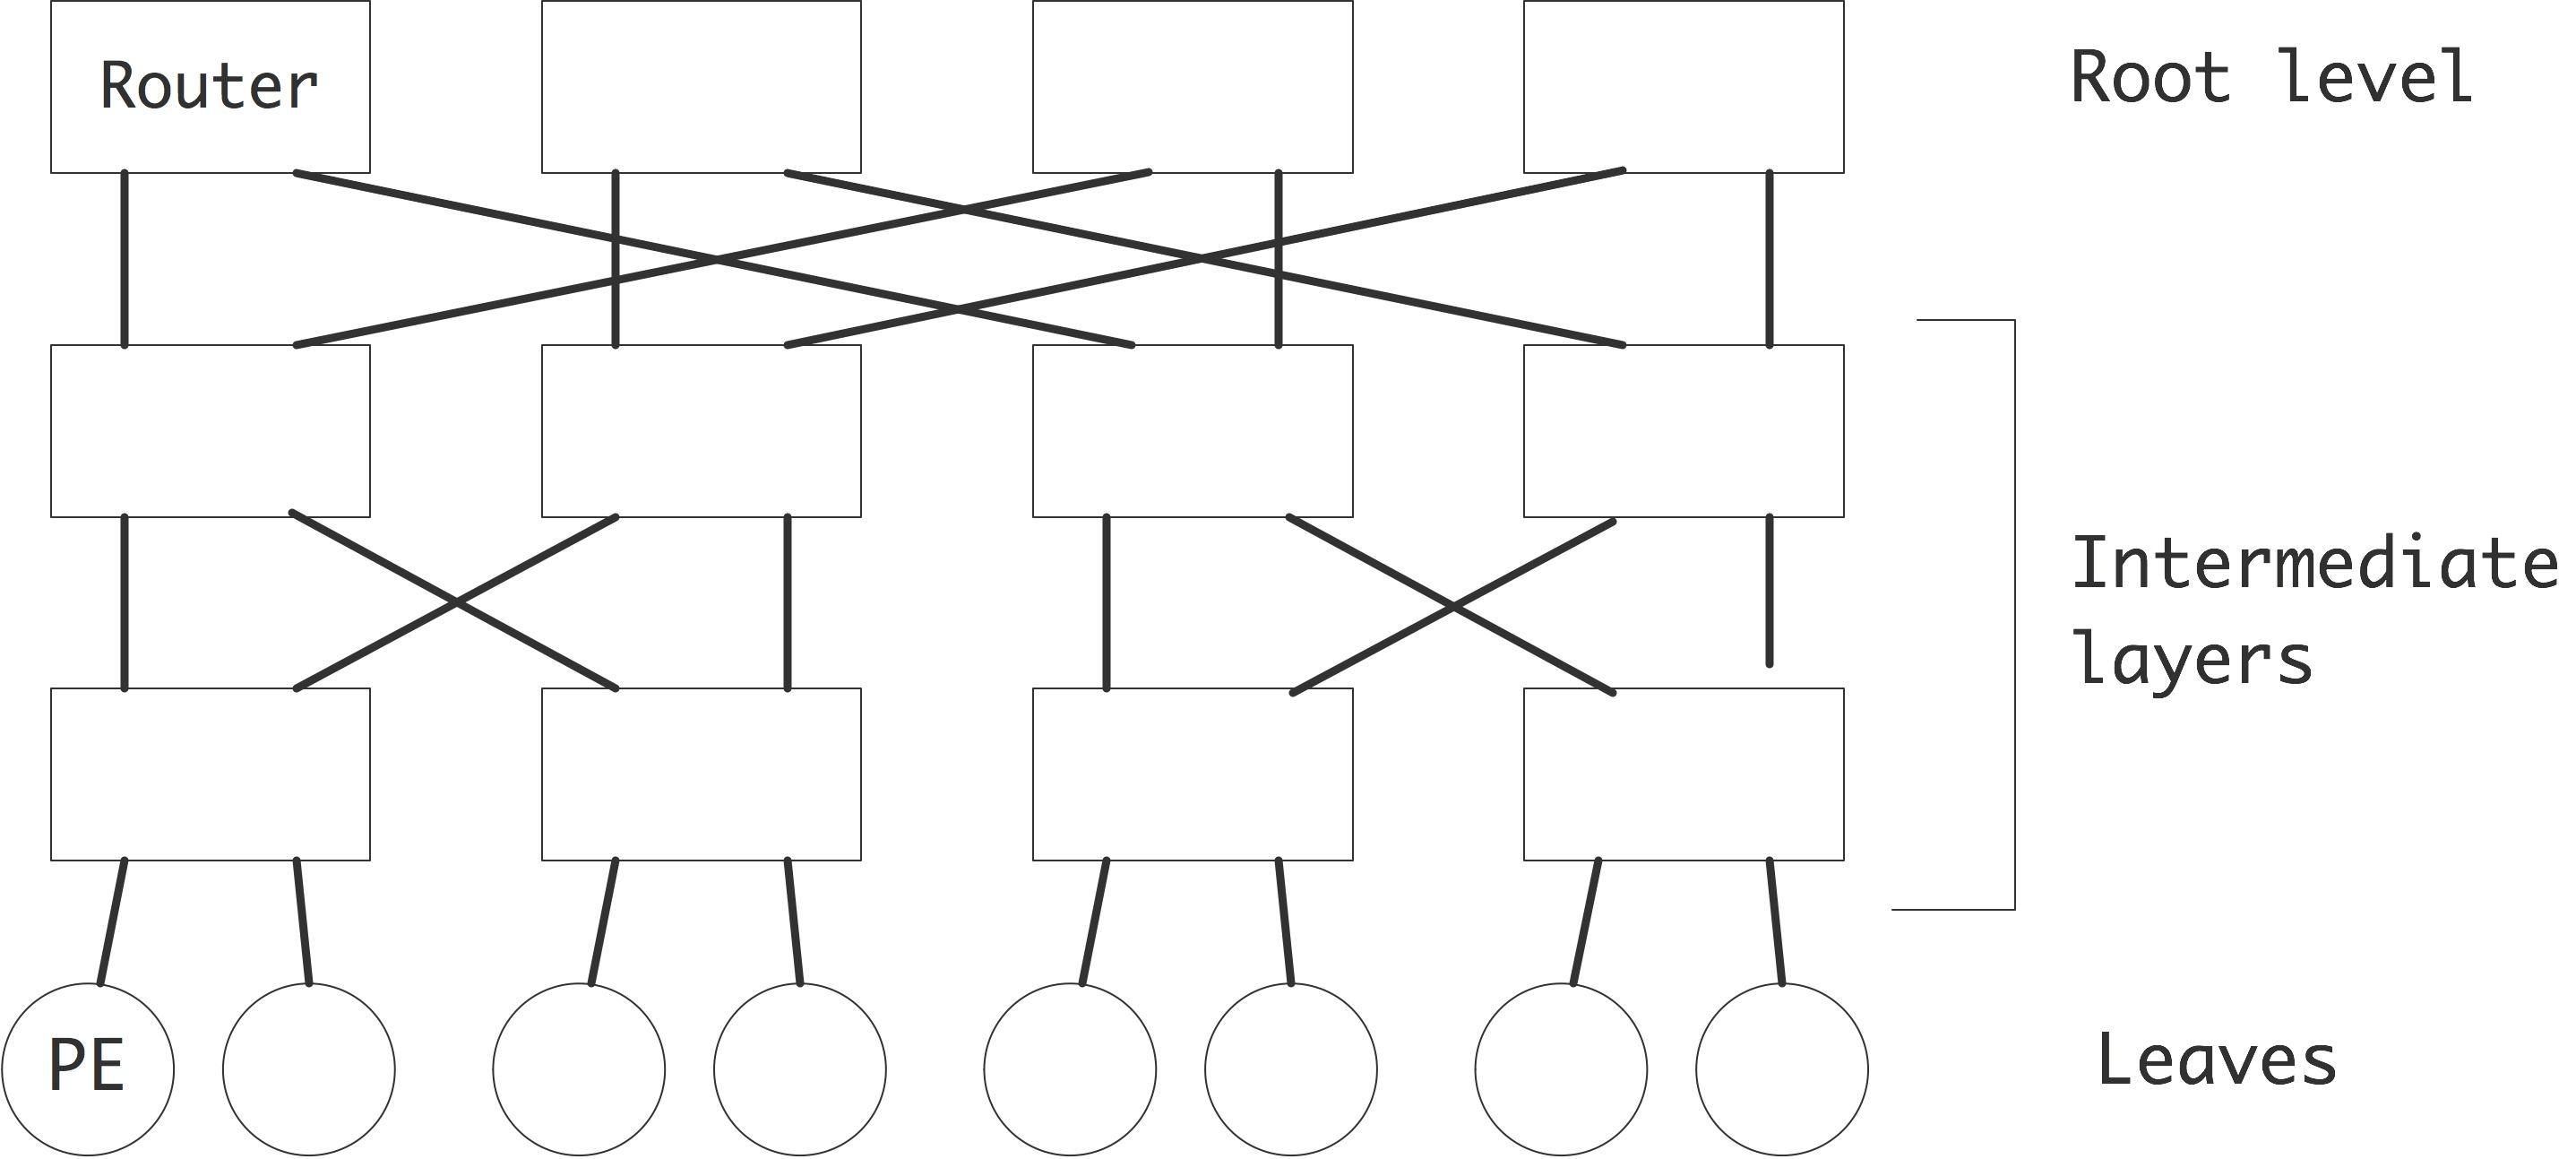
\includegraphics[scale=.11]{graphics/fattree-clos}
  \end{quote}
  \caption{A fat-tree built from simple switching elements}
  \label{fig:fattreeclos}
\end{figure}
This network is equivalent in its bandwidth and routing possibilities
to a fat-tree. Routing algorithms will be slightly more complicated:
in a fat-tree, a data packet can go up in only one way, but here a
packet has to know to which of the two higher switches to route.

This type of switching network is one case of a \indexterm{Clos
  network}~\cite{Clos1953}.

\index{fat tree|)}

\Level 1 {Cluster networks}

The above discussion was somewhat abstract, but in real-life clusters
you can actually see the network designs reflected. For instance,
\emph{fat tree cluster networks}\index{fat tree!clusters based on}
\begin{figure}[th]
  \hbox{%
    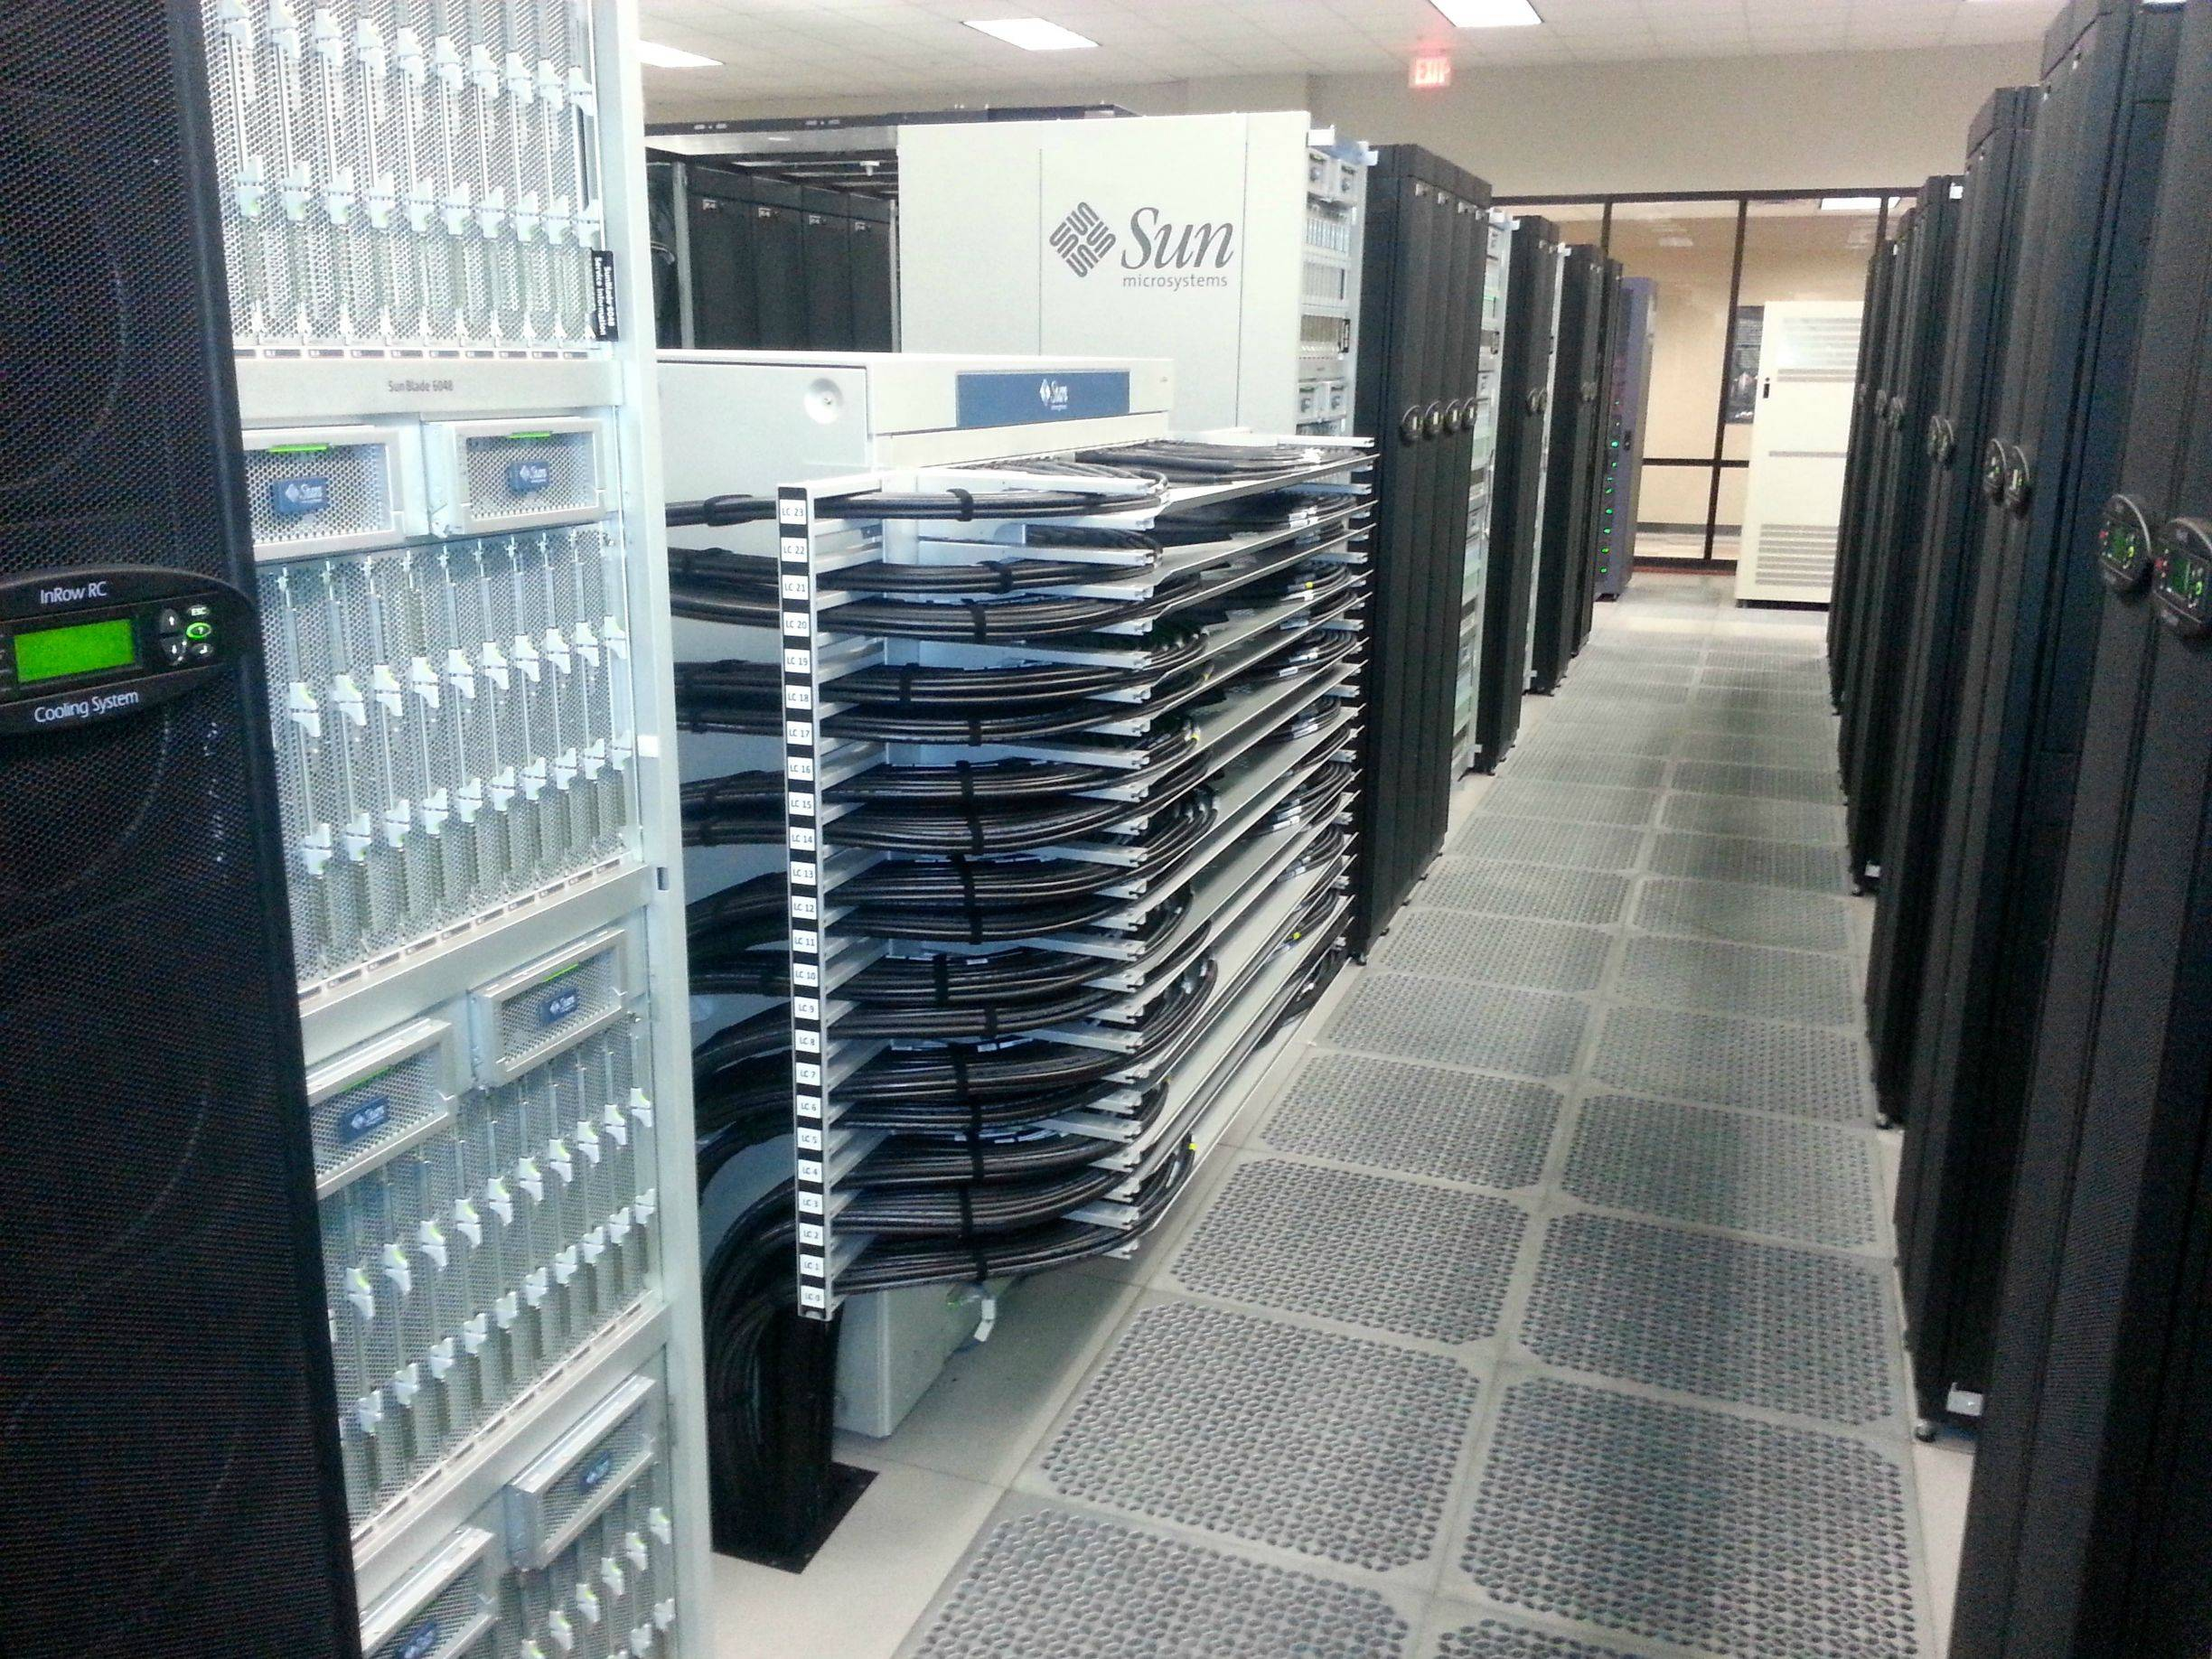
\includegraphics[scale=.08]{rangerswitch}\kern1cm
    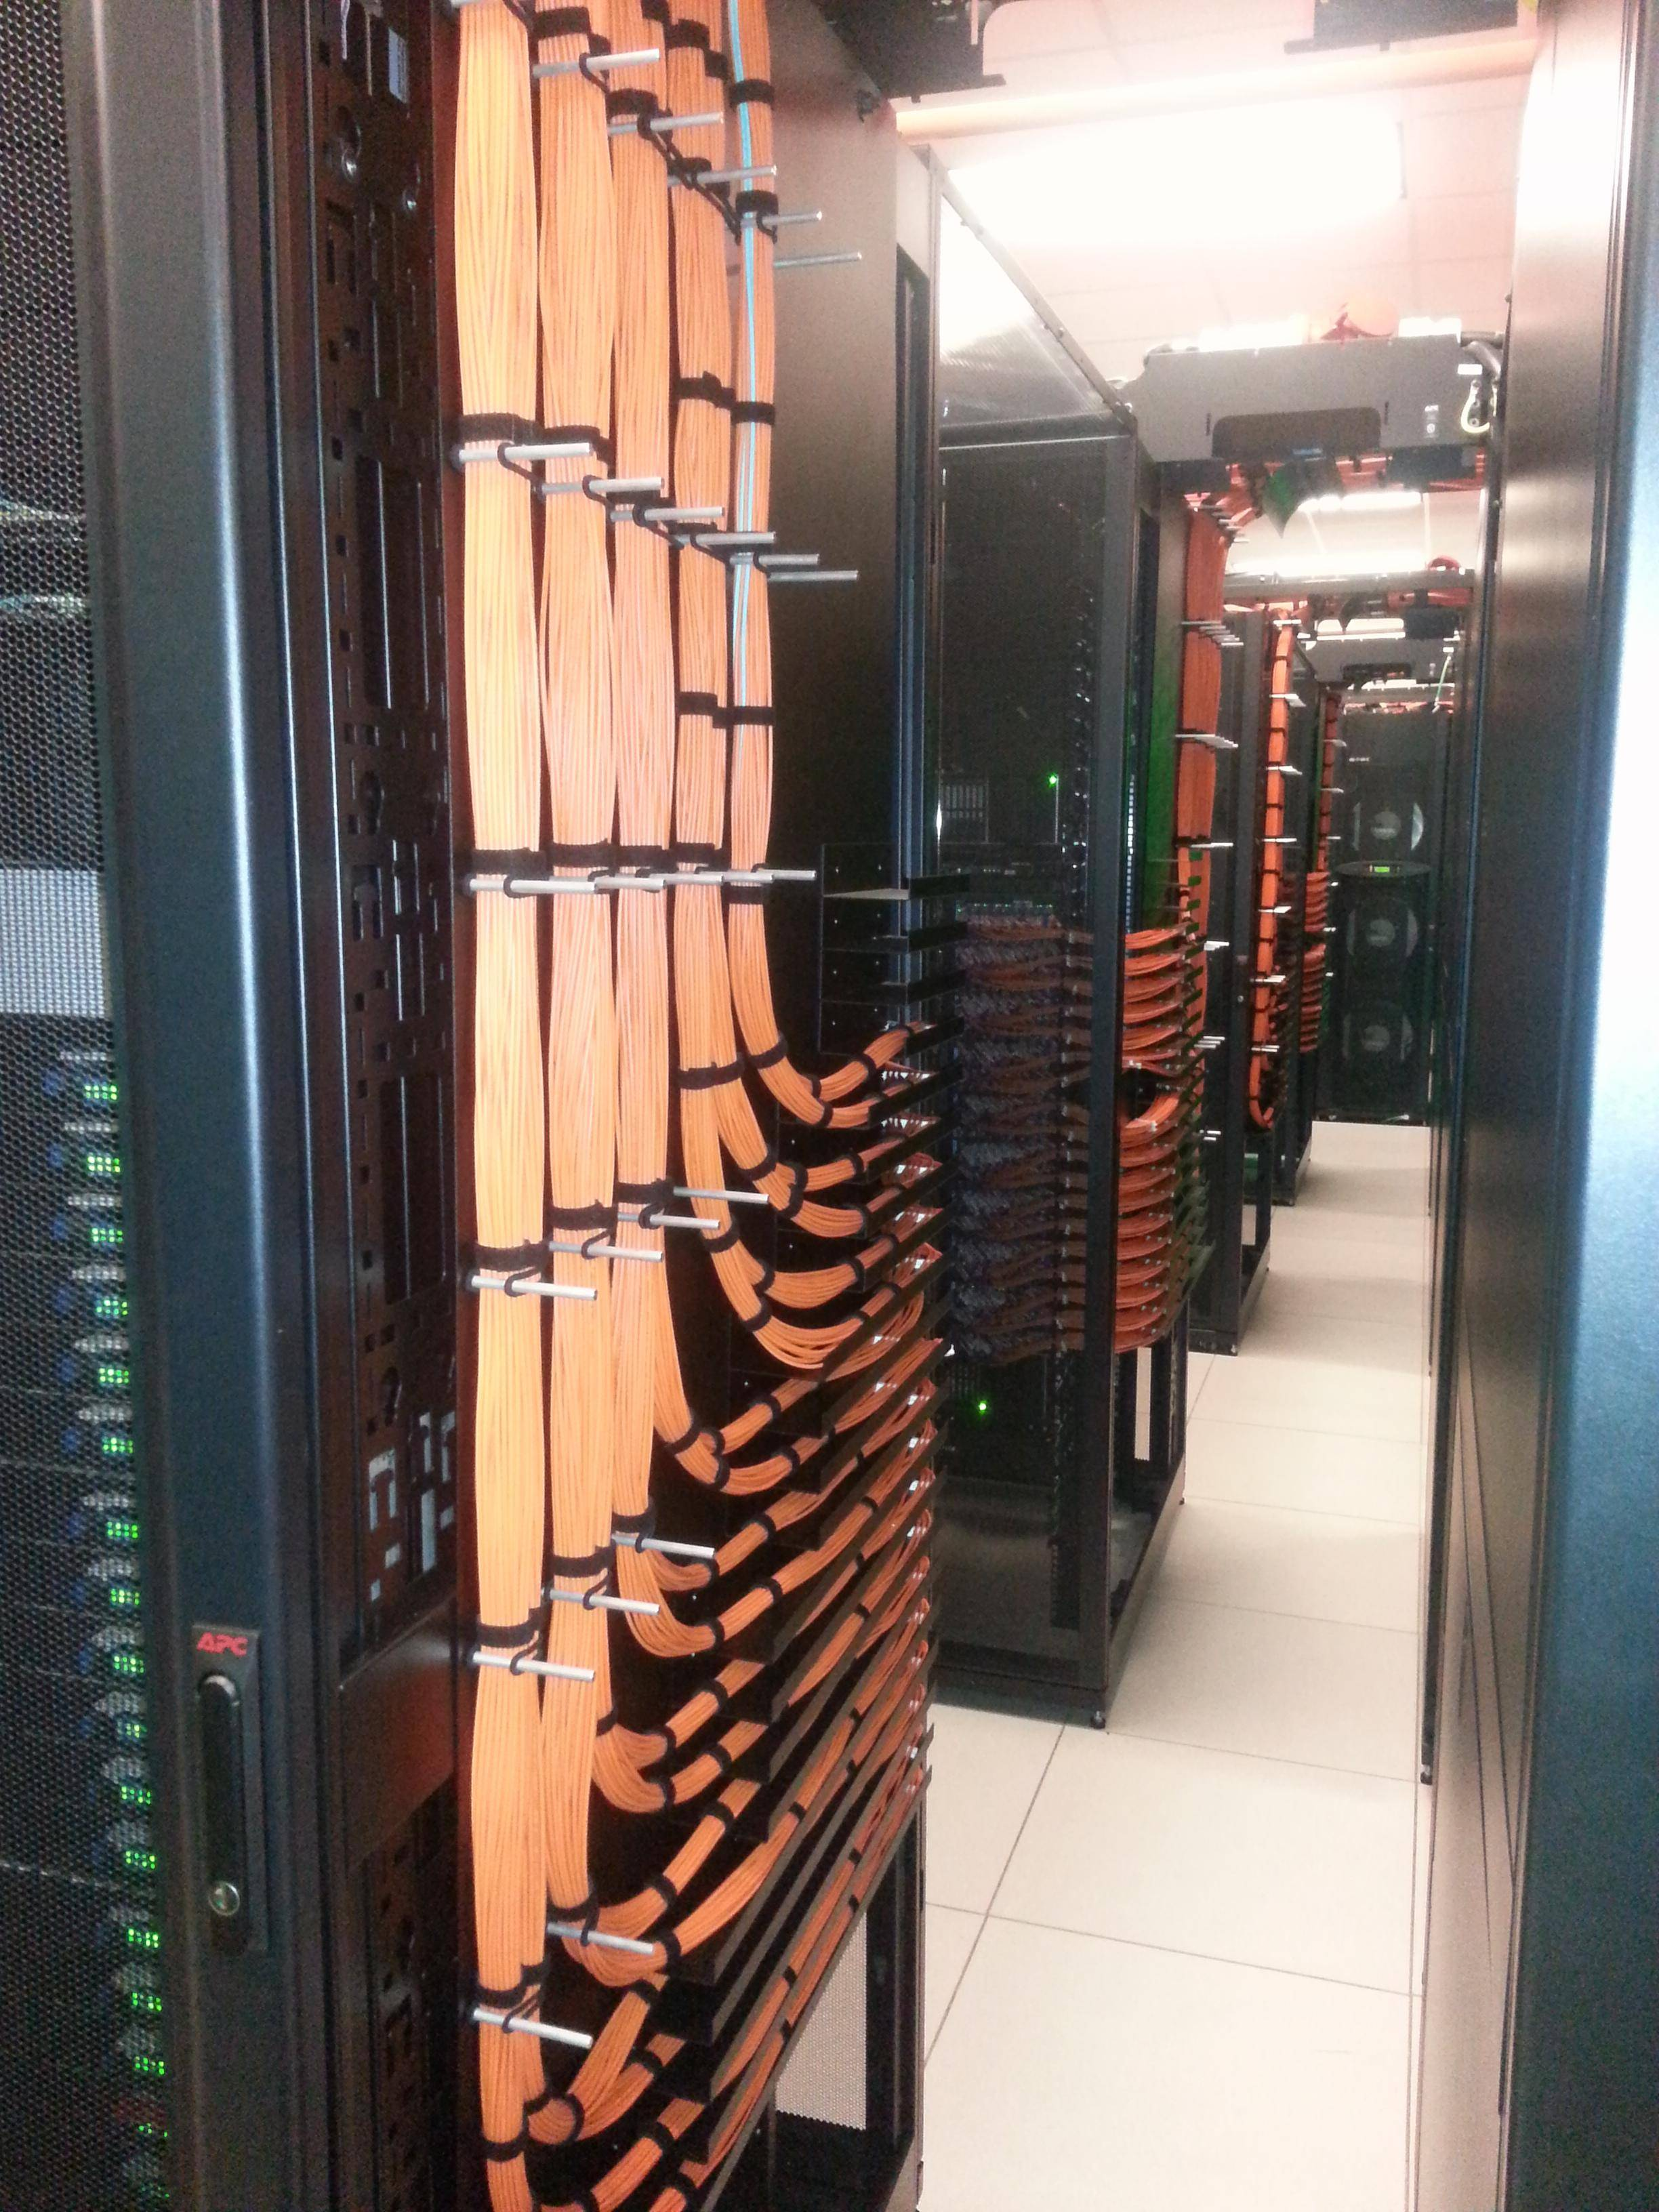
\includegraphics[scale=.08]{stampedeswitches}%
  }
  \caption{Networks switches for the TACC Ranger and Stampede clusters}
  \label{fig:taccswitches}
\end{figure}
will have a central cabinet corresponding to the top level in the tree.
Figure~\ref{fig:taccswitches} shows the switches of the TACC
\emph{Ranger}\index{TACC!ranger cluster} (no longer in service)
and \emph{Stampede}\index{TACC!Stampede cluster} clusters.
In the second picture it can be seen that there are actually
multiple redundant fat-tree networks.

On the other hand, clusters such as the \indextermbus{IBM}{BlueGene},
which is based on a \emph{torus-based cluster}\index{torus!clusters based on},
will look like a collection of identical cabinets, since each contains
\begin{figure}[th]
  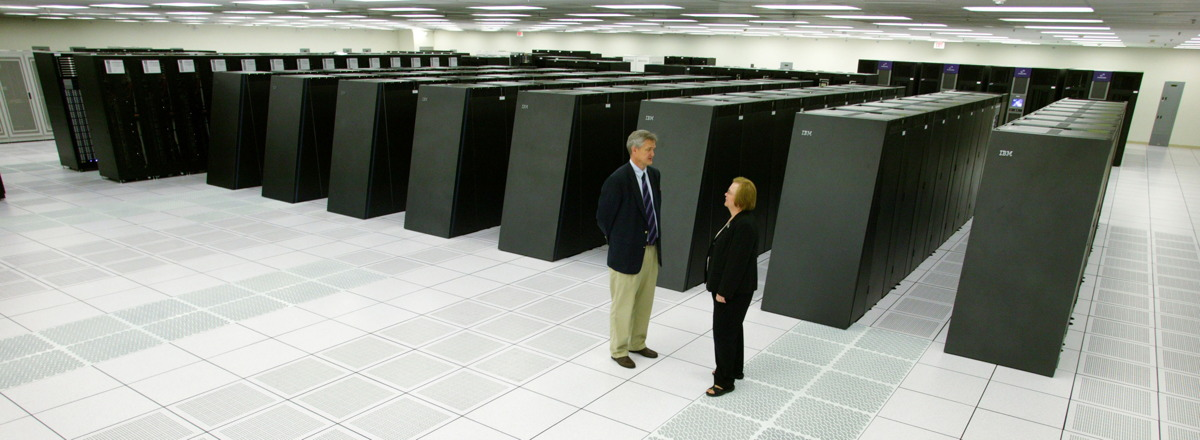
\includegraphics[scale=.5]{bluegenellnl}
  \caption{A BlueGene computer}
%  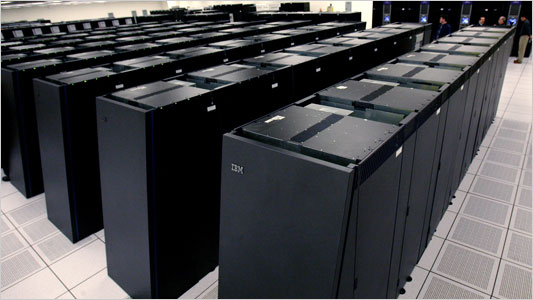
\includegraphics[scale=.5]{bluegene_topview}
%  \caption{An IBM BlueGene/P (Photo: Kimberly White/Reuters)}
  % https://www.llnl.gov/news/newscentercontacts.html
  \label{fig:bluegenep}
\end{figure}
an identical part of the network; see figure~\ref{fig:bluegenep}.

\Level 2 {Case study: Stampede}
\label{sec:stampede-fattree}

As an example of networking in practice, let's consider the
\emph{Stampede}\index{TACC!Stampede cluster} cluster at the Texas
Advanced Computing Center. This can be described as a multi-root
multi-stage fat-tree.
\begin{itemize}
\item Each rack consists of 2 chassis, with 20 nodes each.
\item Each chassis has a leaf switch that is an internal
  \indexterm{crossbar} that gives perfect connectivity between the
  nodes in a chassis;
\item The leaf switch has 36 ports, with 20 connected to the nodes and
  16~outbound. This \indexterm{oversubscription} implies that at most
  16 nodes can have perfect bandwidth when communicating outside the
  chassis.
\item There are 8 central switches that function as 8 independent
  fat-tree root. Each chassis is connected by two connections to a
  `leaf card' in each
  of the central switches, taking up precisely the 16 outbound ports.
\item Each central switch has 18 spine cards with 36 ports each, with
  each port connecting to a different leaf card.
\item Each central switch has 36 leaf cards with 18 ports to the leaf switches
  and 18 ports to the spine cards. This means we can support 648
  chassis, of which 640 are actually used.
\end{itemize}
One of the optimizations in the network is that two connections to the
same leaf card communicate without the latency of the higher tree levels.
This means that 16 nodes in one chassis and 16 nodes in another can
have perfect connectivity.

However, with
\indextermsub{static!routing}, such as used in \indexterm{Infiniband},
there is a fixed port associated with each destination. (This mapping
of destination to port is in the \indextermbus{routing}{tables} in
each switch.) Thus, for some subsets of 16 nodes out 20 possible
destination there will be perfect bandwidth, but other subsets will
see the traffic for two destinations go through the same port.

\Level 1 {Bandwidth and latency}
\label{sec:bwlatency}

The statement above that sending a message can be considered a unit
time operation, is of course unrealistic. A large message will take
longer to transmit than a short one. There are two concepts to arrive
at a more realistic description of the transmission process; we have
already seen this in section~\ref{sec:latencybandwidth} in the context
of transferring data between cache levels of a processor.
\begin{description}
\item[latency] Setting up a communication between two processors takes
  an amount of time that is independent of the message size. The time
  that this takes is known as the \indexterm{latency} of a message.
  There are various causes for this delay.
  \begin{itemize}
  \item The two processors engage in `hand-shaking', to make sure that
    the recipient is ready, and that appropriate buffer space is
    available for receiving the message.
  \item The message needs to be encoded for transmission by the sender,
    and decoded by the receiver.
  \item The actual transmission may take time: parallel computers are
    often big enough that, even at lightspeed, the first byte of a
    message can take hundreds of cycles to traverse the distance
    between two processors.
  \end{itemize}
\item[bandwidth] After a transmission between two processors has been
  initiated, the main number of interest is the number of bytes per
  second that can go through the channel. This is known as the
  \indexterm{bandwidth}. The bandwidth can usually be determined by
  the \indexterm{channel rate}, the rate at which a physical link can
  deliver bits, and the \indexterm{channel width}, the number of
  physical wires in a link. The channel width is typically a multiple
  of 16, usually 64 or~128. This is also expressed by saying that a
  channel can send one or~two 8-byte words simultaneously.
\end{description}

Bandwidth and latency are formalized in the expression
\[ T(n)=\alpha+\beta n \]
for the transmission time of an $n$-byte message. Here, $\alpha$~is
the latency and $\beta$~is the time per byte, that is, the inverse of
bandwidth. Sometimes we consider data transfers that involve
communication, for instance in the case of a \indexterm{collective
  operation}; see section~\ref{sec:collective-cost}. We then extend
the transmission time formula to
\[ T(n)=\alpha+\beta n+\gamma n \]
where $\gamma$ is the time per operation, that is, the inverse of the
\indexterm{computation rate}.

It would also be possible to refine this formulas as
\[ T(n,p) = \alpha+\beta n+\delta p \]
where $p$ is the number of network `hops' that is traversed. However,
on most networks the value of $\delta$ is far lower than of~$\alpha$,
so we will ignore it here. Also, in fat-tree networks
(section~\ref{sec:fat-tree}) the number of hops is of the order of
$\log P$, where $P$~is the total number of processors, so it can never
be very large anyway.

\Level 1 {Locality in parallel computing}
\label{sec:parallel-local}
\index{locality!in parallel computing|(}

In section~\ref{sec:locality} you found a discussion of 
locality concepts in single-processor computing.
The concept of \emph{locality in parallel computing}
comprises all this and a few levels more.

\heading{Between cores; private cache} Cores on modern processors have
private coherent caches. This means that
 it looks like you don't have to worry about locality, since data
  is accessible no matter what cache it is in. However, maintaining coherence
  costs bandwidth, so it is best to keep access localized.

\heading{Between cores; shared cache} The cache that is shared between cores
is one place where you don't have to worry about locality: this is memory that
is truly symmetric between the processing cores.

\heading{Between sockets} The sockets on a node (or motherboard)
appear to the programmer to have shared memory, but this is really 
\indexac{NUMA} access (section~\ref{sec:numa}) since the memory is
associated with specific sockets.

\heading{Through the network structure} Some networks have clear locality effects.
You saw a simple example in section~\ref{sec:graph-theory}, and 
in general it is clear that any grid-type network will favour communication
between `nearby' processors. Networks based on fat-trees seem free of such
contention issues, but the levels induce a different form of locality.
One level higher than the locality on a node, small groups of nodes
are often connected by a \indextermsub{leaf}{switch}, 
which prevents data from going to the central switch.

\index{locality!in parallel computing|)}

\Level 0 {Multi-threaded architectures}
\label{sec:mta}
\input chapters/mta

\Level 0 {Co-processors, including GPUs}
\label{sec:copprocessor}
\index{co-processor|(textbf}

Current CPUs are built to be moderately efficient at just about any
conceivable computation. This implies that by restricting the
functionality of a processor it may be possible to raise its
efficiency, or lower its power consumption at similar
efficiency. Thus, the idea of incorporating a \emph{co-processor}
attached to the \indexterm{host process}
has been explored many times. For instance, Intel's 8086 chip, which
powered the first generation of IBM PCs, could have a numerical
co-processor, the 80287, added to it. This processor was very
efficient at transcendental functions and it also incorporated
\ac{SIMD} technology. Using separate functionality for graphics has also
been popular, leading to the \indexac{SSE} instructions for the x86 processor,
and separate \ac{GPU} units to be attached to the PCI-X bus.

Further examples are the use of co-processors
  for \ac{DSP} instructions, as well as \ac{FPGA} boards which can be
  reconfigured to accommodate specific needs.
Early \indexterm{array processors}
such as the \indextermbus{ICL}{DAP} were also co-processors.

In this section we look briefly at some modern incarnations of this idea,
in particular \acp{GPU}.

\Level 1 {A little history}

Co-processors can be programmed in two different ways: sometimes 
it is seamlessly integrated, and certain instructions are
automatically executed there, rather than on the `host' processor. On
the other hahd, it is also possible that co-processor functions need
to be explicitly invoked, and it may even be possible to overlap
co-processor functions with host functions. The latter case may sound
attractive from an efficiency point of view, but it raises a serious
problem of programmability. The programmer now needs to identify
explicitly two streams of work: one for the host processor and one for
the co-processor.

Some notable parallel machines with co-processors are:
\begin{itemize}
\item The \indextermbus{Intel}{Paragon} (1993) had two processors per
  node, one for communication and the other for computation. These
  were in fact identical, the \indextermbus{Intel}{i860}Intel i860
  processor. In a later revision, it became possible to pass data and
  function pointers to the communication processors.
\item The \indextermbus{IBM}{Roadrunner} at Los Alamos was the first
  machine to reach a PetaFlop\footnote{The \indexterm{Grape computer}
    had reached this point earlier, but that was a special purpose
    machine for molecular dynamics calculations.}. It achieved this
  speed through the use of Cell\index{Cell processor}
  co-processors. Incidentally, the Cell processor is in essence the
  engine of the Sony Playstation3, showing again the commoditization
  of supercomputers (section~\ref{sec:commodity}).
\item The Chinese \indexterm{Tianhe-1A} topped the Top 500 list in
  2010, reaching about 2.5 PetaFlops through the use of
  NVidia\index{NVidia} \acp{GPU}.
\item The \indexterm{Tianhe-2} and the \indextermbus{TACC}{Stampede cluster}
  use \indextermbus{Intel}{Xeon Phi} co-processors.
\end{itemize}
The Roadrunner and Tianhe-1A are examples of co-processors that are
very powerful, and that need to be explicitly programmed independently
of the host CPU. For instance, code running on the \acp{GPU} of the
Tianhe-1A is programmed in \indexterm{CUDA} and compiled separately.

In both cases the programmability problem is further exacerbated by
the fact that the co-processor can not directly talk to the network.
To send data from one co-processor to another it has to be passed to a
host processor, from there through the network to the other host
processor, and only then moved to the target co-processor.

\index{co-processor|)textbf}

\Level 1 {Bottlenecks}

Co-processors often have their own memory, and the
\indextermbus{Intel}{Xeon Phi} can run programs independently, but
more often there is the question of how to access the memory of the
host processor. A~popular solution is to connect the co-processor
through a \indexterm{PCI bus}. Accessing host memory this way is
slower than the direct connection that the host processor has. For
instance, the \emph{Intel Xeon Phi} has a
\emph{bandwidth}\index{Intel!Xeon Phi!bandwidth} of 512-bit wide at
5.5GT per second (we will get to that `GT' in a second), while its
connection to host memory is 5.0GT/s, but only 16-bit wide.

\heading{GT measure} We are used to seeing bandwidth
measured in gigabits per second. For a \indexterm{PCI bus} one often
see the \emph{GT}\index{bandwidth!measure in GT/s} measure. This stands
for giga-transfer, and it measures how fast the bus can change state
between zero and~one.
Normally, every state transition would correspond to a bit, except that
the bus has to provide its own clock information, and if you would send a stream
of identical bits the clock would get confused. Therefore, every 8~bits
are encoded in 10~bits, to prevent such streams. However, this means
that the effective bandwidth is lower than the theoretical number,
by a factor of~$4/5$ in this case.

And since manufacturers like to give a positive spin on things,
they report the higher number.

\Level 1 {GPU computing}
\label{sec:gpu}
\indexacstart{GPU}
\input chapters/gpu
\indexacend{GPU}

\Level 1 {Intel Xeon Phi}
\index{Intel!Xeon Phi|(}

Recently, Intel has released a co-processor, the \emph{Intel Xeon Phi}
(also known by its architecture design as \ac{MIC})
which is expressly designed for numerical computing.
It has both differences and similarities with \acp{GPU}.
\begin{itemize}
\item Both are connected through a \indexterm{PCI-X} bus, which means
  that operations on the device have a considerable latency in
  starting up.
\item The Xeon Phi has general purpose cores, so that it can run whole
  programs; \acp{GPU} has that only to a limited extent (see
  section~\ref{sec:gpu-kernel}).
\item The Xeon Phi accepts ordinary C code.
\item Both architectures require a large amount of SIMD-style
  parallelism, in the case of the Xeon Phi because of the 8-word wide
  \indexac{AVX} instructions.
\item Both devices work, or can work, through \indexterm{offloading}
  from a host program. In the case of the Xeon Phi this can happen
  with OpenMP constructs and \indexterm{MKL} calls.
\end{itemize}

\index{Intel!Xeon Phi|)}

\Level 0 {Load balancing}
\label{sec:load}
\index{load!balancing|(}
\input chapters/load
\index{load!balancing|)}
 
\Level 0 {Remaining topics}

\Level 1 {Distributed computing, grid computing, cloud computing}
\label{sec:cloud}
\index{cloud computing|(}
\index{distributed computing|(}
\SetBaseLevel 2
\input chapters/cloud
\SetBaseLevel 1
\index{cloud computing|)}
\index{distributed computing|)}

\Level 1 {Capability versus capacity computing}
\label{sec:capacity}
\index{capacity computing|(}
\index{capability computing|(}
\input chapters/capability
\index{capacity computing|)}
\index{capability computing|)}

\begin{notready}
\Level 1 {FPGA computing}
\indexacstart{FPGA}
\input chapters/fpga
\indexacend{FPGA}
\end{notready}

\Level 1 {MapReduce}
\label{sec:mapreduce}
\index{MapReduce|(}
\input chapters/mapreduce
\index{MapReduce|)}

\Level 1 {The top500 list}
\label{sec:top500}
\index{top 500|(}
\input chapters/top500
\index{top 500|)}

\Level 1 {Heterogeneous computing}
\label{sec:heterogeneous}
\index{heterogeneous computing|(}
\input chapters/hetero
\index{heterogeneous computing|)}
